% Chapter 5 for e-mailing: same as chapter5_standalone.tex but Appendix A keeps
% the field-station table and OMITS the annotated photo album (the bulk of the
% file size), and Appendix B (text only) is kept. Compile from the repo root:
%   latexmk -pdf -outdir=Standalone/build_lite Standalone/chapter5_lite_standalone.tex
\documentclass{caltech_thesis}
% =============================================================
%  dissertation_preamble.tex
%  Shared package imports and custom commands.
%  \input this file at the top of dissertation.tex ONLY.
% =============================================================

% --- Page geometry -----------------------------------------------------------
% NOTE: caltech_thesis.cls already loads `geometry` itself (1.5in side
% margins, 1in top/bottom, per Caltech's binding/margin requirements), so
% this preamble must NOT load it again with different options -- LaTeX
% would apply whichever load wins and silently ignore the other, which is
% exactly the kind of margin mismatch that gets a thesis bounced at
% submission. If dissertation.tex is ever compiled under a different
% (non-Caltech) document class that does NOT already set geometry, restore
% a line like `\usepackage[margin=1in, letterpaper]{geometry}` here.

% --- Typography --------------------------------------------------------------
\usepackage{lmodern}          % scalable Latin Modern fonts
\usepackage[T1]{fontenc}
\usepackage[utf8]{inputenc}
\usepackage{microtype}        % improved justification
\usepackage{textcomp}         % \textperthousand (per mille, U+2030) below --
                               % most other common unicode punctuation (curly
                               % quotes, en/em dash, degree, plus-minus,
                               % ellipsis) is already handled by inputenc's
                               % utf8 definitions and needs nothing extra.

% A few characters straight from pasted/pandoc-converted source text (e.g.
% Chapter 5's field-report content, which uses literal Greek delta for
% isotope notation like the literal characters "delta-18-O" rather than $\delta^{18}$O) aren't
% in inputenc's default utf8 active-character table and would otherwise be a
% fatal "Unicode character ... not set up for use with LaTeX" error. Map them
% here once, globally, rather than hand-converting every instance in the
% source text (safer -- avoids silently mistyping a value while
% converting).
\usepackage{newunicodechar}
\newunicodechar{δ}{\ensuremath{\delta}}
\newunicodechar{Δ}{\ensuremath{\Delta}}
\newunicodechar{‰}{\textperthousand}

% --- Math --------------------------------------------------------------------
\usepackage{amsmath, amssymb, amsthm}
\usepackage{bm}               % \bm bold math -- used by Chapter 4 (nGibbs methods)
\usepackage{siunitx}          % consistent SI units, e.g. \SI{4.2}{\mega\year}

% --- Figures & tables --------------------------------------------------------
\usepackage{graphicx}
\usepackage{calc}             % arithmetic in lengths (\real{}, +, -, *) -- needed
                               % by Pandoc-generated longtable column specs like
                               % p{(\linewidth - 12\tabcolsep) * \real{0.1951}},
                               % used by Chapter 3's Table 1 (Chapter3/Writing/
                               % HeInSulfides_Main_Body.tex)
\usepackage{float}
\usepackage{placeins}         % \FloatBarrier -- forces pending floats to
                               % resolve before a fixed point (e.g. right
                               % before a non-floating longtable/supertabular
                               % caption) without pinning them to their
                               % source position via [H], which can force a
                               % float onto a page it doesn't fit on and run
                               % it off the bottom margin. See chapter1_SI_
                               % body.tex (fig:predicted-vs-measured-permeation)
                               % for the case this was added for.
\usepackage{booktabs}         % professional table rules
\usepackage{longtable}        % tables that span pages
\usepackage{supertabular}     % multi-page table in Chapter 1 (apatite step-heat
                               % data), shared verbatim with TubeMethodPaper.tex,
                               % which loads supertabular natively via copernicus.cls
\usepackage{multirow}
\usepackage{caption}
\usepackage{subcaption}
\usepackage{array}           % extended column-spec features (>{...},
                              % \newcolumntype); harmless to keep loaded
                              % even though no table currently needs it
                              % now that Chapter 1's widest tables moved
                              % to \chplandscape (landscape) instead of
                              % font-shrinking -- see chapter1_body.tex.
\usepackage{pdflscape}        % \landscape environment, used via the
                              % \chplandscape wrapper (defined per-wrapper
                              % in Chapter1/chapter1.tex and Chapter1/
                              % chapter1_SI.tex) to rotate Chapter 1's
                              % widest tables for extra width in the
                              % thesis only -- the standalone
                              % TubeMethodPaper.tex/Paper/SI.tex define
                              % \chplandscape as a no-op instead, keeping
                              % those journal manuscripts portrait.

% Auto-center every table and shrink its text, without editing individual
% tables. Caltech's required 1.5in side margins leave only a 5.5in text
% width -- narrower than most of these tables were originally drafted for,
% which is why they were rolling off the right edge while left-justified.
%
% NOTE: an earlier version of this tried to wrap every \tabular in an
% adjustbox (\AtBeginEnvironment{tabular}{\begin{adjustbox}{max
% width=\textwidth}}) to hard-guarantee a fit regardless of native column
% widths. That broke the build (fatal "Missing }"/"invalid character"
% errors) -- \AtBeginEnvironment cannot safely wrap an environment that
% takes a mandatory brace argument (tabular's {column-spec}) in another
% such environment, because the injected \begin{adjustbox}{...} steals the
% argument-parsing slot tabular expects for its own column spec. Plain
% declarations (\centering, \footnotesize, \scriptsize -- no arguments of
% their own) are safe here; wrapping one environment inside another via
% this mechanism is not.
\AtBeginEnvironment{table}{\centering\footnotesize}
\AtBeginEnvironment{longtable}{\centering\scriptsize}
\AtBeginEnvironment{supertabular}{\centering\scriptsize}
\setlength{\tabcolsep}{3pt}   % default is 6pt -- tighter padding buys back
                              % real width on many-column numeric tables

% A few of the widest tables use fixed-width p{...} columns (in cm) rather
% than content-driven columns, so shrinking the font alone doesn't reclaim
% any width -- those still need a per-table \resizebox wrap (done directly
% in the affected .tex files, not here) for a hard guarantee of fit.
\graphicspath{
  {figures/}
  {Chapter1/Figures/source/}
  {Chapter1/Figures/generated/}
  {Chapter2/Figures/source/}
  {Chapter2/Figures/generated/}
  {Chapter3/Figures/source/}
  {Chapter3/Figures/generated/}
  {Chapter3/Figures/generated/step_heat_regressions/}
  {Chapter4/Figures/}
  {Chapter4/Figures/generated/}
  {Chapter5/Figures/}
  {Chapter5/Figures/source/}
  {Chapter5/Figures/generated/}
  {ChapterA/Figures/}
}

% --- Colors & hyperlinks -----------------------------------------------------
\usepackage[dvipsnames]{xcolor}
\usepackage[
  colorlinks = true,
  linkcolor  = NavyBlue,
  citecolor  = OliveGreen,
  urlcolor   = Maroon,
  pdftitle   = {From Surface to Core},
  pdfauthor  = {Ben Thyer},
]{hyperref}
\usepackage{doi}

% --- Bibliography ------------------------------------------------------------
% Name-truncation rule (discipline convention, not a Caltech requirement --
% Caltech's thesis guidelines explicitly leave reference/citation style to
% "the style current in the thesis writer's discipline," only requiring it be
% used consistently throughout): 2-author works print both names; 3+-author
% works truncate to the first author + "et al." (maxnames=2, minnames=1).
% uniquelist=true is the standard biblatex safety net for the case where two
% DIFFERENT works would otherwise truncate to an identical-looking citation
% (e.g. "Smith et al., 2020" for two unrelated Smith-led 2020 papers) -- it
% expands the printed name list just enough to tell them apart (e.g. "Smith,
% Jones, et al." vs. "Smith, Brown, et al.") rather than appending a/b/c
% letters. True letter disambiguation (2020a / 2020b) already happens
% automatically -- with no extra config -- whenever two entries share the
% exact same full author list AND year (e.g. a genuine same-author same-year
% duplicate); it does not, by default, cover the "different authors, same
% truncated display" case, which is what uniquelist handles instead. As of
% this writing, a scan of references.bib found zero actual collisions under
% the new maxnames=2 rule, so this is a forward-looking safety net, not a
% fix for a live problem.
%
% maxbibnames is set high (effectively "no truncation") so the References
% list at the end always spells out every author, regardless of how the
% in-text citation truncates -- maxnames/minnames above only govern in-text
% \citep/\citet, not the bibliography.
\usepackage[
  backend    = biber,
  style      = authoryear,   % change to e.g. agu or geology if preferred
  sorting    = nyt,
  maxnames   = 2,
  minnames   = 1,
  maxbibnames = 99,
  uniquelist = true,
  giveninits = true,
  uniquename = init,
  natbib     = true,         % provides \citep/\citet/\citealp (natbib syntax),
                              % which Chapter 1's shared body (reused from
                              % TubeMethodPaper.tex) uses throughout. Without
                              % this, biblatex only offers its own
                              % \parencite/\textcite commands.
]{biblatex}
\addbibresource{references.bib}   % master .bib file — keep alongside dissertation.tex

% --- Header / footer ---------------------------------------------------------
\usepackage{fancyhdr}
\pagestyle{fancy}
\fancyhf{}
\fancyhead[LE,RO]{\thepage}
\fancyhead[RE]{\textit{\leftmark}}
\fancyhead[LO]{\textit{\rightmark}}
\renewcommand{\headrulewidth}{0.4pt}

% caltech_thesis.cls sets headsep to a very tight ~0.25in - 1em (roughly
% 6pt), tuned for its own default page style, which puts only a bare page
% number in the header. Since fancyhdr above instead puts the italicized
% chapter/section title (\leftmark/\rightmark) in the header, long titles
% that wrap to a second line collide with the body text below. Calling
% \geometry{} again (rather than re-\usepackage-ing it) only updates the
% keys given here and safely recomputes \textheight to match -- it does
% NOT reload/conflict with the page-margin setup the NOTE above warns
% about. headheight=30pt comfortably fits two lines of a 12pt header;
% headsep=18pt keeps a clean gap below it. If a chapter title ever needs
% a third header line, bump headheight further (e.g. to 42pt).
\geometry{headheight=30pt, headsep=18pt}

% --- Chapter / section formatting --------------------------------------------
% NOTE: caltech_thesis.cls (memoir-based) already defines its own official
% Caltech chapter styling -- centered, italic small-caps "Chapter I" numbering
% in Roman numerals via \chapnamefont/\chaptitlefont/\printchapterheading -- so
% titlesec's \titleformat{\chapter} override below has been disabled. Loading
% titlesec's chapter redefinition on top of memoir's own chapter-heading system
% is a known source of conflicts/incompatibility warnings. Re-enable this only
% if compiling Chapter files under a plain `book`/`report` class instead.
% \usepackage{titlesec}
% \titleformat{\chapter}[display]
%   {\normalfont\Large\bfseries}{\chaptertitlename\ \thechapter}{20pt}{\Huge}
% \titlespacing*{\chapter}{0pt}{40pt}{20pt}

% --- Per-chapter Supplementary Information (SI) -------------------------------
% Each chapter's SI (Chapter<N>/chapter<N>_SI.tex) is \input{} immediately
% after that chapter's main body, inside the SAME \chapter{} -- it is not a
% chapter of its own. Two problems that creates, and how these commands fix
% them:
%
% 1. Visually, the SI used to just continue as the next plain \section{},
%    indistinguishable from the chapter's own sections. \SItitlepage{...}
%    gives it a proper divider/title page first (unnumbered, no header, own
%    page), the way a book's appendix or backmatter would get one.
%
% 2. Numerically, its \section headings used to continue the chapter's own
%    numbering (...7, 8, 9...), so a reader landing mid-SI from a link or a
%    flipped-to page couldn't tell from the running header alone whether they
%    were still in the chapter proper or in its supplement. The `ChapterSI`
%    environment resets the section counter and switches \thesection to a
%    "<chapter>.<n>s" format for everything between \begin{ChapterSI} and
%    \end{ChapterSI} (e.g. the SI's first section becomes "1.1s" instead of
%    continuing on from wherever the main text left off). \thesubsection
%    inherits this automatically, since its default definition already
%    builds on \thesection. \S\ref{}/running headers/the ToC all pick this
%    up for free, because \setcounter and \renewcommand are both local by
%    default, and LaTeX environments are always wrapped in their own group,
%    so everything reverts automatically at \end{ChapterSI} with no matching
%    "restore" step to maintain. (The *next* chapter's own section numbering
%    isn't at risk even without that revert -- \chapter{} always resets
%    \c@section to 0 globally on its own, regardless of whatever it was left
%    at.)
%
%    NOTE on naming, two dead ends hit along the way, for the record:
%     (a) This is a `\newenvironment`, not a pair of \newcommand{\beginSI}/
%         \newcommand{\endSI} macros -- LaTeX reserves all command names of
%         the form \end<word> for environment closers, so
%         \newcommand{\endSI}{...} is flatly illegal ("Or name \end...
%         illegal", LaTeX2e kernel restriction, independent of memoir/
%         caltech_thesis.cls). Defining it as a proper environment sidesteps
%         that and is the more idiomatic way to express "everything between
%         these two markers" in LaTeX anyway.
%     (b) The environment is named `ChapterSI`, not `SI` -- \newenvironment{SI}
%         would auto-generate \SI as its begin-code control sequence, which
%         collides with siunitx's own \SI{value}{unit} command (loaded
%         above, e.g. \SI{4.2}{\mega\year}). `ChapterSI` generates
%         \ChapterSI/\endChapterSI instead, which don't collide with
%         anything.
%    Repeat this same \SItitlepage{...}/\begin{ChapterSI}...\end{ChapterSI}
%    pattern for Chapter 2 and beyond's SI wrappers.
\newcommand{\SItitlepage}[1]{%
  \clearpage
  \thispagestyle{empty}
  \vspace*{\fill}
  \begin{center}
    {\Huge\bfseries Supplementary Information}\\[1.5em]
    {\Large for Chapter \thechapter: \itshape #1}
  \end{center}
  \vspace*{\fill}
  \clearpage
}
\newenvironment{ChapterSI}{%
  \setcounter{section}{0}
  \renewcommand{\thesection}{\thechapter.\arabic{section}s}
}{}

% --- Appendix ----------------------------------------------------------------
% NOT loaded explicitly: memoir (which caltech_thesis.cls is built on) already
% emulates the `appendix` package internally with its own default options, so
% an explicit `\usepackage[toc, page]{appendix}` here causes a fatal "Option
% clash for package appendix" error. The `\begin{appendices}...\end{appendices}`
% environment used in dissertation.tex still works via memoir's built-in
% emulation without loading the package separately.

% --- Miscellaneous -----------------------------------------------------------
\usepackage{enumitem}
% pdflscape already loaded above (Figures & tables section) for \chplandscape
\usepackage{pdfpages}         % include external PDFs (field maps, etc.)
\usepackage{soul}             % \hl{} highlighting -- used once in Chapter 2's
                               % shared body (chapter2_body.tex)
\usepackage{lineno}           % line numbers — comment out for final version
% \linenumbers

% --- Custom commands ---------------------------------------------------------
\newcommand{\degC}{\ensuremath{^\circ\mathrm{C}}}
\newcommand{\He}{\textsuperscript{4}He}
\newcommand{\UThHe}{U--Th/He}
\newcommand{\fO}{\ensuremath{f_{\mathrm{O_2}}}}
\newcommand{\fS}{\ensuremath{f_{\mathrm{S_2}}}}
\newcommand{\fH}{\ensuremath{f_{\mathrm{H_2O}}}}
\newcommand{\Ea}{\ensuremath{E_a}}
\newcommand{\todo}[1]{\textcolor{red}{\textbf{[TODO: #1]}}}

\title{Chapter 5: Draaikraal}\author{Ben J. Thyer}\copyyear{2026}
% Photo numbers would link to the (omitted) album: make them plain text.
\newcommand{\ChFivePhotoLink}[2]{#2}
% Downsampled copies of the three large vector maps (25 MB -> 3 MB) come first.
\graphicspath{{Standalone/lite_figs/}{Chapter5/Figures/}{Chapter5/Figures/source/}{Chapter5/Figures/generated/}{ChapterA/Figures/}}
\begin{document}
\mainmatter
\setcounter{chapter}{4}
% =============================================================
%  Chapter 5 — Draaikraal Field Study
%  "Field Studies Reveal Synmagmatic Deformation and Extensive
%   Crustal Contamination of the Upper Critical Zone, Recessive
%   Lower Main Zone, and Floor Rocks at the Margin of the
%   Bushveld Complex at Draaikraal, Mpumalanga, South Africa"
%
%  Mirrors the Chapter 1 / Chapter 3 pattern: this wrapper \input{}s
%  the shared content files in Chapter5/Writing/ -- chapter5_abstract.tex
%  and chapter5_body.tex -- so the science is written and edited in
%  exactly one place. Edit those files (or Chapter5/Figures/
%  write_chapter5_data_table.py for the data tables), not this one, to
%  change the text, figures, or tables.
%
%  Reorganized 2026-09-01 from the raw field-report text/data that had
%  been dropped directly in Chapter5/ (Draaikraal 2023 BJT.tex/.xlsx,
%  structural_map.pdf) into the Chapter1-3 Writing/Figures/Tables/
%  Workspace layout; see chapter5_body.tex's own header comment for the
%  full provenance/content-change notes. This chapter previously held a
%  stub for the ML-thermodynamics ("nGibbs") chapter, which has moved to
%  Chapter4/chapter4.tex (displacing DustMAP, now shelved at
%  Manuscripts/DustMAP/ and out of the thesis) -- see Chapter4/chapter4.tex's
%  header comment.
%
%  NOTE: Do NOT include \documentclass or \begin{document} here.
%        This file is \input{} into dissertation.tex.
% =============================================================

\chapter{Field Studies Reveal Synmagmatic Deformation and Extensive Crustal Contamination of the Upper Critical Zone, Recessive Lower Main Zone, and Floor Rocks at the Margin of the Bushveld Complex at Draaikraal, Mpumalanga, South Africa}
\label{ch:draaikraal}

% --- Chapter abstract / summary -----------------------------------------------
\begin{quote}
  \itshape
  % =============================================================
%  chapter5_abstract.tex
%  Chapter abstract for Chapter 5 (Draaikraal field study). Extracted
%  verbatim from the original field-report abstract in
%  Chapter5/Workspace/Draaikraal 2023 BJT.tex (the raw pandoc export of
%  Draaikraal Report.docx) -- text unchanged, only the surrounding
%  title/author front matter (handled by chapter5.tex's own \chapter{}
%  and the thesis title page) and the "Abstract" heading itself
%  (handled by the \begin{quote} wrapper in chapter5.tex) were removed.
% =============================================================

The paleoproterozoic Rustenburg Layered Suite (RLS) of the Bushveld
Magmatic Province in northeast South Africa is the largest layered
igneous intrusion in the world, and contains the world's largest source
of platinum group elements as well as important reserves of chromium,
vanadium, titanium, and iron. It is exceptionally well-preserved, and
has been the subject of intense study and debate for generations.
Studies focusing on the intrusion's margin have been especially fruitful
in informing geologists' understanding of igneous petrogenesis and
intrusion mechanisms, modes, and tempos of layered mafic intrusions and
plutonic rocks more generally. The phaneritic RLS is stratigraphically
divided into four zones based on geochemistry and modal mineralogy: the
Lower, Critical, Main, and Upper Zones. These zones are often thought to
have been constructed at differing times and from different magmatic
sources and processes. Thus, the intersection of these stratigraphically
defined zones at the intrusion's margin are particularly interesting
locations for detailed field work. This field study focuses on several
unusual but understudied structural and geomorphic features occurring at
the economically significant intersection of the Main and Critical Zones
with the intrusion's margin in the well-exposed Eastern Limb near the
village of Draaikraal, Mpumalanga, South Africa: the Kliprivier synform,
the Draaikraal Lineament, and the unexpected recessive topography of the
Main Zone in the agricultural valley surrounding the village of
Draaikraal.

The Kliprivier Synform represents a series of modestly rotated plutonic
rocks with conspicuously absent modal layering, and country rocks that
include Quartzite, calc-silicate hornfels, and fine-grained Marginal
Zone gabbros. The country rocks appear to be displaced \textasciitilde{}
1 km into the plutonic RLS near the mapped intersection of the Critical
and Main Zones. The Draaikraal Lineament (named here) is a linear
feature of recessive topography stretching from the country rocks beyond
the intrusion's margin to the middle Main Zone. It overlaps with the
Kliprivier Synform and separates typical, resistant Main Zone
gabbronorites to the north from the recessive Main Zone gabbronorites to
the south in the agricultural valley around Draaikraal. Using structural
measurements and correlation of mottled anorthosite marker beds of the
lower Main Zone, I find that the mottled anorthosite marker beds are
concordant with the floor rocks at the intrusions margin and are not
displaced across the Draaikraal Lineament. I argue that the Kliprivier
Synform is a synmagmatic monocline that formed due to lopolithic
deformation of the country rock roof by the intrusion of Critical Zone
sills before the formation of the UG2 chromitite and overlying Merensky
Reef and Main Zones. The orientation of the Draaikraal Lineament is very
similar to the surface-projection of the axial plane of the Kliprivier
Monocline, which likely continues at depth. The relative recessive
topography of the Draaikraal Lineament and the Main Zone to the south is
argued to be the result of higher degrees of contamination by
hydrothermal fluids than the more resistant Main Zone gabbronorites of
the surrounding area. The rocks at the Draaikraal Lineament are
envisaged to be fluxed with upwardly migrating fluids that were trapped
by the Critical Zone roof, escaping by exploiting the structural
weakness of the Kliprivier Monocline. The agricultural valley to the
south of the lineament is simply envisaged to be relatively contaminated
by melting and devolatilizing sediments at the proximal floor, whereas
the resistant Main Zone to the north was relatively buffered by
interaction with such fluids by the thick Critical Zone rocks that
underlie it there.

\end{quote}

% --- Field-data table macros (auto-generated -- see the file header) ----------
% \ChFiveFieldStationTable / \ChFiveStructuralMeasurementsTable. Defined here
% (rather than only where first used) following the Chapter 3 pattern, so
% they are available wherever chapter5_body.tex's Sample and Station Data
% section (\S\ref{sec:ch5-sample-station-data}) invokes them. Regenerate via
% Chapter5/Figures/write_chapter5_data_table.py after any change to
% Tables/Draaikraal 2023 BJT.xlsx.
% =============================================================
%  chapter5_data_table.tex -- AUTO-GENERATED, DO NOT EDIT BY HAND.
%  Written by Chapter5/Figures/write_chapter5_data_table.py from
%  Chapter5/Tables/Draaikraal 2023 BJT.xlsx ('Geotagged Stratigraphy').
%  Regenerate after any change to the spreadsheet:
%    python3 Chapter5/Figures/write_chapter5_data_table.py
%  \input{} by Chapter5/chapter5.tex (defines the macro); invoked from
%  Chapter5/Writing/chapter5_SI_body.tex.
% =============================================================
\providecommand{\ChFivePhoto}[1]{#1}
\newcommand{\ChFiveFieldStationTable}{%
\begingroup
\edef\ChFiveSavedFootnote{\the\value{footnote}}\setcounter{footnote}{0}
\renewcommand{\thefootnote}{\arabic{footnote}}
\begin{scriptsize}
\fontsize{7.5}{8.6}\selectfont
\renewcommand{\arraystretch}{0.9}
\setlength{\tabcolsep}{3pt}
\begin{longtable}{@{}>{\raggedright\arraybackslash}p{1.95cm} r r r r l l l >{\raggedright\arraybackslash}p{1.5cm}@{}}
\caption{Field observations of the Draaikraal campaign (July 2023). Lat./Lon.: WGS84, decimal degrees. Elev.: elevation (m). 
Unit: final interpreted map unit and Lith.: lithology code (\S\ref{sec:ch5-lithologic-descriptions}). 
Structure: bedding (Bed.), cleavage (Clv.), contact (Cont.) or modal layering (M.L.), as strike/dip with strike an azimuth from north. 
Photos: field photograph numbers; those reproduced in \S\ref{sec:ch5-SI-photo-album} or as figures are links, the others are in the 
supplementary photo album. Field descriptions and notes are footnotes to the observation name, at the foot of the page. `--': not recorded.}\label{tab:ch5-field-stations}\\
\toprule
Name & Ht. & Lat. & Lon. & Elev. & Unit & Lith. & Structure & Photos \\
\midrule
\endfirsthead
\multicolumn{9}{@{}l}{\textit{Table~\ref{tab:ch5-field-stations} (continued)}} \\
\toprule
Name & Ht. & Lat. & Lon. & Elev. & Unit & Lith. & Structure & Photos \\
\midrule
\endhead
\midrule
\multicolumn{9}{r@{}}{\textit{continued on next page}} \\
\endfoot
\bottomrule
\endlastfoot
RZ22 & -933 & -25.24760 & 30.11812 & 2146 & Rz & Msp & -- & -- \\
QZ27 & -724 & -25.24040 & 30.10576 & 2076 & Rz & Qz & -- & -- \\
QZ7 & -706 & -25.23020 & 30.11221 & 1958 & Rz & Qz & -- & -- \\
RZ54 & -700 & -25.23980 & 30.10496 & 2044 & Rz & Msp & -- & -- \\
CONT MARG E Q W?\footnote{\scriptsize Quartzite. Quartzite follows topo line locally here.} & -697 & -25.22880 & 30.11288 & 1960 & Rz & Qz & -- & -- \\
D3NB & -683 & -25.22540 & 30.11481 & 1960 & Rz & Qz & Bed. 145/30 & -- \\
QZ1 & -676 & -25.22530 & 30.11455 & 1956 & Rz & Qz & -- & -- \\
D3NA\footnote{\scriptsize Compass trouble, resolved.} & -674 & -25.22590 & 30.11390 & 1929 & Rz & Qz & Bed. 120/30 & -- \\
RZ43 & -669 & -25.23920 & 30.10392 & 2015 & Rz & Msp & -- & -- \\
D7NC\footnote{\scriptsize Alternating quartzite-marginal zone photo, not very good one.} & -661 & -25.23900 & 30.10369 & 2010 & Rz & Qz & -- & -- \\
RZ8 & -654 & -25.22500 & 30.11369 & 1945 & Rz & Msp & -- & -- \\
D3NC\footnote{\scriptsize No faulting; the quartz and marginal zone is interbedded.} & -649 & -25.22510 & 30.11337 & 1940 & Rz & QzMsp & -- & \ChFivePhoto{34} \\
RZ21 & -644 & -25.22500 & 30.11326 & 1947 & Rz & Msp & -- & -- \\
RZ24 & -643 & -25.23900 & 30.10279 & 1997 & Rz & Msp & -- & -- \\
RZ36 & -642 & -25.23860 & 30.10304 & 1995 & Rz & Msp & -- & -- \\
QZ112 & -639 & -25.23860 & 30.10289 & 1995 & Rz & Qz & -- & -- \\
D3SF\footnote{\scriptsize Qz-Px Pegmatite. Hosted in migmatitic quartzite. Schist banding deformed around pegmatite.} & -638 & -25.22610 & 30.11207 & 1929 & Rz & ScP & -- & \ChFivePhoto{37}, \ChFivePhoto{38} \\
SCHIS & -636 & -25.22580 & 30.11224 & 1937 & Rz & Sc & -- & -- \\
QZ2 & -631 & -25.22510 & 30.11260 & 1950 & Rz & Qz & -- & -- \\
QZ3 & -631 & -25.22460 & 30.11297 & 1954 & Rz & Qz & -- & -- \\
RZ11 & -629 & -25.22490 & 30.11266 & 1952 & Rz & Msp & -- & -- \\
QZ6 & -629 & -25.22520 & 30.11238 & 1946 & Rz & Qz & -- & -- \\
QZ5 & -626 & -25.22480 & 30.11255 & 1950 & Rz & Qz & -- & -- \\
RZ31 & -625 & -25.22600 & 30.11153 & 1926 & Rz & Msp & -- & -- \\
RZ33 & -622 & -25.22460 & 30.11252 & 1946 & Rz & Msp & -- & -- \\
D3SE\footnote{\scriptsize Fine grained, light rock. Dacite? Silicified. Pockmarks weathering proud in paleovertical pipes.} & -621 & -25.22460 & 30.11251 & 1950 & Rz & Msp & -- & \ChFivePhoto{36}, \ChFivePhoto{40} \\
D3SD\footnote{\scriptsize Migmatized quartzite. Banded. Light bands of quartz preserve original sedimentary texture. Grains rounded and 2 mm. Some bands pink (feldspar) some green (chlorite, epidote?)} & -619 & -25.22450 & 30.11247 & 1946 & Rz & ScQz & -- & \ChFivePhoto{35} \\
RZ71 & -617 & -25.22690 & 30.11044 & 1911 & Rz & Msp & -- & -- \\
SCHIST & -615 & -25.22440 & 30.11236 & 1944 & Rz & Sc & -- & -- \\
QZ4 & -615 & -25.22430 & 30.11241 & 1945 & Rz & Qz & -- & -- \\
RZ41 & -614 & -25.22410 & 30.11254 & 1948 & Rz & Msp & -- & -- \\
RZ110 & -614 & -25.23840 & 30.10183 & 1976 & Rz & Msp & -- & -- \\
RZ51 & -614 & -25.22290 & 30.11342 & 1945 & Rz & Msp & -- & -- \\
RZ61 & -599 & -25.22550 & 30.11068 & 1907 & Rz & Msp & -- & -- \\
RZ32 & -588 & -25.22590 & 30.10982 & 1900 & Rz & Msp & -- & -- \\
QZ26 & -575 & -25.23760 & 30.10054 & 1948 & Rz & Qz & -- & -- \\
D7SE\footnote{\scriptsize Silicate Pegmatite. within migmatized qzite very close to magnesite skarn. Myrmekitic quartz-K-spar, huge OPX, small vibrant rare green and blue crystals: apatite, CPX, beryl?} & -569 & -25.23690 & 30.10081 & 1946 & Rz & ScP & -- & \ChFivePhoto{70}, \ChFivePhoto{71} \\
SHIST & -569 & -25.23690 & 30.10078 & 1947 & Rz & ScP & -- & -- \\
RZUP & -565 & -25.23740 & 30.10019 & 1935 & Rz & ScPMsp & -- & -- \\
D7SD\footnote{\scriptsize Magnesite Skarn. within migmatized qzite. In ground, hard to tell if dike or concordant with schist host.} & -559 & -25.23740 & 30.09991 & 1936 & Rz & ScP & -- & \ChFivePhoto{69} \\
D2NC\footnote{\scriptsize Contact. On this ridge, there are multiple bands of quartzites with Marginal Zone between them. Is the marginal zone a sill between layers of quartzite, or is there a fault? (Update, I think it’s a strike-slip(?) fault striking E-W dipping to the South with a component of left-lateral shear along the ridge)} & -555 & -25.22110 & 30.11222 & 1993 & Rz & QzMsp & -- & \ChFivePhoto{14}, \ChFivePhoto{23}, \ChFivePhoto{28} \\
D7NA\footnote{\scriptsize Fine marginal gabbronorite with shearing pegmatite veins. sheared pegmatite veins in pockets/pipes orthogonal to bedding, paleo-up. This layer is just above migmatized quartzite and just below fine magnetic marginal zone. Represents fluid transport from migmatized sedimentary rocks, origin of resistance banding? Strike and Dip are for migmatized Qz.} & -552 & -25.23700 & 30.09985 & 1924 & Rz & QzMsp & Bed. 220/25 & \ChFivePhoto{67} \\
SCH1 & -551 & -25.23700 & 30.09984 & 1930 & Rz & ScP & -- & -- \\
RZMAG & -549 & -25.23690 & 30.09979 & 1919 & Rz & Msp & -- & -- \\
RZ & -532 & -25.22390 & 30.10878 & 1909 & Rz & Msp & -- & -- \\
D1ND\footnote{\scriptsize Bladed iridescent white crystals (Plagioclase) in 2 cm thick planar features intersect orthogonally in outcrop. The plagioclase planes are surrounded by 10 cm zone of oikocrystic augite. The southwestern limb pinches in and out and occasionally overlaps itself in parallel, a la boudinage.} & -507 & -25.23730 & 30.09753 & 1926 & Rz & Msp & -- & \ChFivePhoto{6} \\
D1NC\footnote{\scriptsize Note that all marginal zone rocks are characterized by dark resistance bands, perhaps cataclastic, reflecting warm-brittle deformation with finely recrystallized zones. They stand proud. They frequently strike E-W, secondarily, NE-SW, tertiarily.  NW-SE, but can vary and appear pretty random. This feature is diagnostic of the marginal zone.} & -500 & -25.23720 & 30.09730 & 1924 & Rz & Msp & -- & -- \\
RZ3 & -485 & -25.22250 & 30.10765 & 1910 & Rz & Msp & -- & -- \\
RLS & -481 & -25.22350 & 30.10665 & 1890 & Cz & Pg & -- & -- \\
RZ1 & -481 & -25.22030 & 30.10931 & 1973 & Rz & Msp & -- & -- \\
D1Sb\footnote{\scriptsize Common Marginal zone Medium-fine grained gabbronorite.} & -479 & -25.23690 & 30.09644 & 1891 & Rz & Msp & -- & \ChFivePhoto{19} \\
D1A\footnote{\scriptsize Fine-grained Magnetite Gabbro with gabbronoritic blocks. Fine-grained magnetite gabbro includes rounded, elongate blocks of oikocrystic gabbronorite preferentially horizontally imbricated, $\sim$6-10 cm along axis. Also a bunch of rounded gabbronorite inclusions that may represent the spherical aggregates of the TBM.} & -479 & -25.23690 & 30.09644 & 1891 & Rz & MspTB & -- & \ChFivePhoto{4} \\
MZ3 & -478 & -25.22290 & 30.10699 & 1902 & Cz & Pg & -- & -- \\
D2SB\footnote{\scriptsize Sampled because quartzite here all have iron stained interiors. The weathered exteriors are clear. Quartzites served as a conduit for mobilized iron-rich fluids?} & -477 & -25.21950 & 30.10983 & 2004 & Rz & Qz & -- & -- \\
RZ2 & -470 & -25.22270 & 30.10679 & 1901 & Rz & Msp & -- & -- \\
D2SH\footnote{\scriptsize Schist with Skarn. Swirled and deformed schist with marginal zone, with thin clear banding. Non-magnetic. Xenolith? Associated with skarn pegmatite veins: 60\% Feldspar, 40\% amphibole? Big very dark crystals that I think I see 120 degree cleavage on… Likely devolatilizing xenolith.} & -469 & -25.22070 & 30.10839 & 1950 & Rz & ScP & -- & \ChFivePhoto{29}, \ChFivePhoto{30} \\
RQCONT & -465 & -25.21920 & 30.10955 & 2014 & Rz & QzMsp & -- & -- \\
RZ20 & -456 & -25.23540 & 30.09654 & 1903 & Rz & Msp & -- & -- \\
RZ5 & -441 & -25.23760 & 30.09423 & 1918 & Rz & Msp & -- & -- \\
D2ND\footnote{\scriptsize Measurable bedding planes at top of ridge: Strike: 265, Dip: 25. Also, One bedding plane preserved lovely sedimentary ripples striking E-W.} & -440 & -25.21820 & 30.10918 & 2020 & Rz & Qz & Bed. 175/25 & -- \\
D11SA\footnote{\scriptsize Coarse grained gabbronorite. Is it critical-margin zone? Are resistance bands chromite bearing?} & -440 & -25.23770 & 30.09405 & 1899 & Rz & Msp & -- & -- \\
QZ FOOLLOW TOPO & -433 & -25.21900 & 30.10814 & 1990 & Rz & Qz & -- & -- \\
RZ4 & -431 & -25.23700 & 30.09419 & 1906 & Rz & Msp & -- & -- \\
RZ6 & -430 & -25.23860 & 30.09298 & 1923 & Rz & Msp & -- & -- \\
D2NE\footnote{\scriptsize Different strike, same dip. Strike: 315, dip: 25. Quartzites are rotated around the top of the ridge. NW-SE vertical fault or E-W South dipping fault can neatly explain rotation.} & -426 & -25.21670 & 30.10968 & 2031 & Rz & Qz & Bed. 225/25 & -- \\
D4NB\footnote{\scriptsize Contact between floor quartzite and marginal zone. Bed plane of quartzite measured.} & -422 & -25.24150 & 30.09048 & 1932 & Rz & QzMsp & Bed. 240/25 & \ChFivePhoto{52} \\
QZ51 & -417 & -25.21880 & 30.10754 & 1993 & Rz & Qz & -- & -- \\
D10NK & -415 & -25.24210 & 30.08966 & 1917 & Rz & Qz & Bed. 235/25 & -- \\
RZ7 & -413 & -25.23870 & 30.09213 & 1915 & Rz & Msp & -- & -- \\
D4SA\footnote{\scriptsize Contact between marginal zone and migmatized quartzite. Migmatitic quartzite $\sim$10m thick. At contact is non-magnetic leucocratic gneiss, then fine magnetic marginal zone: 10cm, then coarse grained marginal zone: 30 cm, then common fine marginal zone.} & -412 & -25.24090 & 30.09036 & 1895 & Rz & QzMsp & -- & \ChFivePhoto{50}, \ChFivePhoto{51} \\
SCHI & -403 & -25.24040 & 30.09025 & 1882 & Rz & Sc & -- & -- \\
QZ61 & -402 & -25.21890 & 30.10676 & 1980 & Rz & Qz & -- & -- \\
QZ41 & -402 & -25.21870 & 30.10691 & 1987 & Rz & Qz & -- & -- \\
QZ & -395 & -25.21680 & 30.10808 & 2001 & Rz & Qz & -- & -- \\
QZ29 & -393 & -25.24210 & 30.08861 & 1907 & Rz & Qz & -- & -- \\
QZ71 & -391 & -25.21900 & 30.10613 & 1975 & Rz & Qz & -- & -- \\
RZ28 & -388 & -25.24200 & 30.08845 & 1906 & Rz & Msp & -- & -- \\
SCH & -387 & -25.24010 & 30.08972 & 1870 & Rz & Sc & -- & -- \\
RZ12 & -381 & -25.23990 & 30.08955 & 1866 & Rz & Msp & -- & -- \\
D2SA\footnote{\scriptsize Common Main Zone Coarse Grained Gabbronorite (Office interp: Leucogabbronorite; porphyritic gabbronorite) On Dirt road to Kliprivier Farms, Boulder piles outcropping of main zone. These rocks are the building materials for much of the structures in the area. Weathering is quite distinct from Marginal zone. Both have exfoliation/onion skin weathering. Main Zone is prouder, forming impressive rounded boulders like a granite. Weathered faces have distinct dalmatian pattern. A large boulder (float) at this outcrop contains a characteristic pyroxene “tennisball”, a well-known marker at the base of the Main Zone.} & -380 & -25.23000 & 30.09696 & 1860 & Cz & PgTB & -- & -- \\
RZ35 & -380 & -25.21890 & 30.10566 & 1965 & Rz & Msp & -- & -- \\
D2SF\footnote{\scriptsize Coarse Grained Magnetite Gabbro. Actually I am now thinking this sample is similar to the magnetite gabbro D1Sa, but coarser grained. That sample too had zones of coarse grains, and this one also had blocks of oikocrystic augite.} & -379 & -25.21550 & 30.10829 & 1994 & Rz & Msp & -- & \ChFivePhoto{24} \\
RZ42 & -379 & -25.21940 & 30.10519 & 1950 & Rz & Msp & -- & -- \\
QZ8 & -377 & -25.21920 & 30.10529 & 1954 & Rz & Qz & -- & -- \\
RZ9 & -370 & -25.23920 & 30.08952 & 1850 & Rz & Msp & -- & -- \\
RAT & -368 & -25.23630 & 30.09174 & 1883 & Rz & Msp & -- & -- \\
RZ511 & -368 & -25.21970 & 30.10442 & 1935 & Rz & Msp & -- & -- \\
RZLQZR & -366 & -25.21960 & 30.10440 & 1938 & Rz & QzMsp & -- & -- \\
RZ53 & -362 & -25.21930 & 30.10448 & 1945 & Rz & Msp & -- & -- \\
RZ113 & -359 & -25.24170 & 30.08722 & 1876 & Rz & Msp & -- & -- \\
IS1 & -358 & -25.23030 & 30.09577 & 1868 & IS & IS & -- & -- \\
RZ62 & -355 & -25.21960 & 30.10390 & 1934 & Rz & Msp & -- & -- \\
D2SG\footnote{\scriptsize Norite. Weathering more closely resembles main zone than nearby marginal zone, but this rock does not look like main zone to me. Non-magnetic.} & -352 & -25.21390 & 30.10811 & 1956 & Cz & Dcg & -- & \ChFivePhoto{27} \\
QZ9 & -352 & -25.22000 & 30.10342 & 1929 & Rz & Qz & -- & -- \\
SCI & -350 & -25.23900 & 30.08890 & 1888 & Rz & Sc & -- & -- \\
D9NE & -348 & -25.25130 & 30.07965 & 1929 & Rz & Qz & Bed. 180/15 & -- \\
QZ10 & -347 & -25.22000 & 30.10320 & 1928 & Rz & Qz & -- & -- \\
SCH11 & -343 & -25.24070 & 30.08725 & 1881 & Rz & Sc & -- & -- \\
RZ27 & -341 & -25.24060 & 30.08725 & 1882 & Rz & Msp & -- & -- \\
D9SD\footnote{\scriptsize Fine Grained Marginal Norite. Sampled for prominent resistance band for later analyses.} & -340 & -25.25150 & 30.07907 & 1912 & Rz & Msp & -- & \ChFivePhoto{95} \\
QZ11 & -339 & -25.21970 & 30.10308 & 1938 & Rz & Qz & -- & -- \\
SCH2 & -338 & -25.23940 & 30.08802 & 1887 & Rz & Sc & -- & -- \\
RZ82 & -338 & -25.23960 & 30.08784 & 1886 & Rz & Msp & -- & -- \\
D9NC\footnote{\scriptsize Chloritized Norite. Plag, OPX, abundant phlogopite, alteration grade lessens up section.} & -335 & -25.25180 & 30.07858 & 1908 & Rz & Msp & -- & -- \\
QZ12 & -334 & -25.21970 & 30.10285 & 1939 & Rz & Qz & -- & -- \\
D9NF\footnote{\scriptsize Fine Grained Marginal norite. Droplet forms of coarse pyroxenite xenoliths, pegmatite inclusions?} & -333 & -25.25050 & 30.07951 & 1918 & Rz & MspTB & -- & \ChFivePhoto{96} \\
RZ23 & -331 & -25.21720 & 30.10466 & 1957 & Rz & Msp & -- & -- \\
RZ72 & -330 & -25.21940 & 30.10291 & 1940 & Rz & Msp & -- & -- \\
RZ81 & -318 & -25.21920 & 30.10248 & 1940 & Rz & Msp & -- & -- \\
RZ19 & -316 & -25.21700 & 30.10410 & 1948 & Rz & Msp & -- & -- \\
RZ25 & -312 & -25.24970 & 30.07913 & 1910 & Rz & Msp & -- & -- \\
D9NG\footnote{\scriptsize Paleovertical Pegmatite Dike Photograph, Marginal zone coarsens upsection towards quartzite.} & -312 & -25.24980 & 30.07904 & 1910 & Rz & Msp & -- & \ChFivePhoto{97}, \ChFivePhoto{98} \\
D5NC\footnote{\scriptsize Cleavage.} & -299 & -25.21880 & 30.10195 & 1946 & Rz & Msp & Clv. 145/25 & \ChFivePhoto{57} \\
RZ44 & -290 & -25.24030 & 30.08497 & 1844 & Rz & Msp & -- & -- \\
RZ18 & -286 & -25.21730 & 30.10245 & 1940 & Rz & Msp & -- & -- \\
RZ91 & -280 & -25.21900 & 30.10086 & 1928 & Rz & Msp & -- & -- \\
QZ31 & -264 & -25.21640 & 30.10209 & 1933 & Rz & Qz & -- & -- \\
QZ28 & -252 & -25.24750 & 30.07796 & 1893 & Rz & Qz & -- & -- \\
RZ10 & -252 & -25.21880 & 30.09972 & 1929 & Rz & Msp & -- & -- \\
QZ13 & -248 & -25.21950 & 30.09891 & 1907 & Rz & Qz & -- & -- \\
D5SB\footnote{\scriptsize Amphibole Gabbro. Weakly magnetic, amphibole bearing? Rock clearly rotten.} & -248 & -25.21430 & 30.10287 & 1919 & Cz & A & -- & -- \\
D9NH & -244 & -25.24740 & 30.07764 & 1895 & Rz & Qz & Bed. 230/35 & -- \\
QZ23 & -242 & -25.21610 & 30.10128 & 1932 & Rz & Qz & -- & -- \\
QZ14 & -241 & -25.21960 & 30.09852 & 1907 & Rz & Qz & -- & -- \\
QZ15 & -233 & -25.21970 & 30.09807 & 1907 & Rz & Qz & -- & -- \\
RPEG1 & -229 & -25.21390 & 30.10229 & 1907 & Cz & Dcg & -- & -- \\
RZ111 & -223 & -25.21950 & 30.09777 & 1902 & Rz & Msp & -- & -- \\
D7NF\footnote{\scriptsize Pegmatitic gabbronorite. large (5 cm) oikocrystic pyroxene.} & -218 & -25.21350 & 30.10206 & 1906 & Cz & Dcg & Bed. 180/10 & \ChFivePhoto{73} \\
QZ110 & -215 & -25.21610 & 30.10002 & 1923 & Rz & Qz & -- & -- \\
QZ113 & -214 & -25.24740 & 30.07621 & 1874 & Rz & Qz & -- & -- \\
RZ121 & -213 & -25.21890 & 30.09779 & 1911 & Rz & Msp & -- & -- \\
QZ16 & -213 & -25.21910 & 30.09763 & 1908 & Rz & Qz & -- & -- \\
QZ17 & -211 & -25.21880 & 30.09778 & 1915 & Rz & Qz & -- & -- \\
RZ13 & -209 & -25.21860 & 30.09780 & 1909 & Rz & Msp & -- & -- \\
QZ18 & -205 & -25.21850 & 30.09772 & 1914 & Rz & Qz & -- & -- \\
D9NI\footnote{\scriptsize Schist (Pebble marker?) well mixed clasts of schists, zones of pink felsic melt.} & -204 & -25.24670 & 30.07624 & 1865 & Rz & ScMsp & -- & \ChFivePhoto{99}, \ChFivePhoto{100}, \ChFivePhoto{101}, \ChFivePhoto{102} \\
QZ19 & -200 & -25.21860 & 30.09741 & 1912 & Rz & Qz & -- & -- \\
RZ112 & -199 & -25.24650 & 30.07613 & 1865 & Rz & Msp & -- & -- \\
D7NG\footnote{\scriptsize Pegmatitic gabbronorite. Here magnetic, slightly upsection ($\sim$2 m) rocks non-magnetic. Large (30 cm) blobs of pyroxenite rimmed by anorthosite. Pyroxene/Anorthosite ranging from 1/4 to 4. Included blocks with preserve resistance banding.} & -197 & -25.21220 & 30.10208 & 1905 & Cz & Dcg & Clv. 230/15 & \ChFivePhoto{72}, \ChFivePhoto{73}, \ChFivePhoto{74}, \ChFivePhoto{75} \\
SCHI1 & -193 & -25.24620 & 30.07609 & 1863 & Rz & Sc & -- & -- \\
RZQZLEFT & -193 & -25.21920 & 30.09654 & 1887 & Rz & QzMsp & -- & -- \\
QZ20 & -187 & -25.21880 & 30.09663 & 1901 & Rz & Qz & -- & -- \\
RZ14 & -185 & -25.21870 & 30.09657 & 1900 & Rz & Msp & -- & -- \\
RZ15 & -175 & -25.21840 & 30.09636 & 1895 & Rz & Msp & -- & -- \\
RZ26 & -173 & -25.24550 & 30.07565 & 1856 & Rz & Msp & -- & -- \\
MZ11 & -166 & -25.22800 & 30.08851 & 1837 & Cz & Pg & -- & -- \\
D5SA\footnote{\scriptsize Thought it looked like the "dark facies" main zone in the field,. Compare to D25g (porphyritic gabbronorite), Quartzite in float (alluvial)} & -166 & -25.21540 & 30.09820 & 1903 & Cz & UD & -- & -- \\
D6SL\footnote{\scriptsize Porphyritic gabbronorite. In notes, described as main zone porphyritic gabbronorite. However these rocks are structurally beneath chrome layers. Closer inspection reveals that pyroxenes are often oikocrystic and large... Incompletely formed Mottled Anorthosite?} & -165 & -25.21490 & 30.09851 & 1892 & Cz & Pg & -- & -- \\
RZ16 & -162 & -25.21870 & 30.09548 & 1887 & Rz & Msp & -- & -- \\
QZ22 & -161 & -25.21810 & 30.09591 & 1898 & Rz & Qz & -- & -- \\
D5NE & -160 & -25.21870 & 30.09537 & 1883 & Rz & Msp & Clv. 125/25 & -- \\
RZ17 & -154 & -25.21950 & 30.09445 & 1875 & Rz & Msp & -- & -- \\
QZ21 & -153 & -25.21950 & 30.09444 & 1875 & Rz & Qz & -- & -- \\
QZ25 & -147 & -25.21770 & 30.09553 & 1877 & Rz & Qz & -- & -- \\
D6SG\footnote{\scriptsize Magnetite pegmatite. Host rock magnetic. Pegmatite weathers proud, cutting the rock paleo-up, "sandy" texture in host rock.} & -146 & -25.21840 & 30.09491 & 1872 & Rz & QzMsp & -- & \ChFivePhoto{60} \\
D6NK\footnote{\scriptsize Porphyritic gabbronorite.} & -145 & -25.21500 & 30.09749 & 1888 & Cz & Pg & Clv. 120/5 & -- \\
D7SH\footnote{\scriptsize Sulfide-pyroxenite.} & -144 & -25.21020 & 30.10109 & 1898 & Cz & Px & -- & \ChFivePhoto{78} \\
D6SH\footnote{\scriptsize Coarse-grained Feldspathic Pyroxenite. Non-magnetic, Floor of critical zone? "Flatreef"?} & -144 & -25.21770 & 30.09534 & 1871 & Cz & Dcg & -- & \ChFivePhoto{62} \\
D6SI\footnote{\scriptsize Coarse-grained Feldspathic Pyroxenite. Coarser grained rocks here are more rotten.} & -144 & -25.21770 & 30.09534 & 1871 & Cz & Dcg & -- & \ChFivePhoto{61} \\
QZ111 & -140 & -25.21760 & 30.09526 & 1869 & Rz & Qz & -- & -- \\
QZ24 & -139 & -25.21800 & 30.09487 & 1869 & Rz & Qz & -- & -- \\
RPEQ & -135 & -25.21480 & 30.09718 & 1883 & Cz & Dcg & -- & -- \\
PEG & -133 & -25.21140 & 30.09968 & 1893 & Cz & Dcg & -- & -- \\
D6NJ\footnote{\scriptsize Pegmatite gabbronorite.} & -132 & -25.21540 & 30.09655 & 1880 & Cz & Dcg & Clv. 150/10 & \ChFivePhoto{63} \\
RPEG & -130 & -25.21540 & 30.09644 & 1877 & Cz & Dcg & -- & -- \\
RZ34 & -124 & -25.21910 & 30.09334 & 1858 & Rz & Msp & -- & -- \\
RZ37 & -120 & -25.24380 & 30.07447 & 1840 & Rz & Msp & -- & -- \\
RZ52 & -118 & -25.22040 & 30.09203 & 1846 & Rz & Msp & -- & -- \\
D7NI\footnote{\scriptsize Pyroxene tennisballs in Gabbronorite. Structurally below chromite?} & -100 & -25.20893 & 30.09996 & 1876 & Cz & PgTB & -- & \ChFivePhoto{79}, \ChFivePhoto{119} \\
D7SJ\footnote{\scriptsize Gabbronorite. small amount of interstitial CPX. Transitional zone?} & -100 & -25.20890 & 30.09995 & 1876 & Cz & Pg & -- & -- \\
MZPOR & -96 & -25.20910 & 30.09963 & 1873 & Cz & Pg & -- & -- \\
CZ3 & -94 & -25.20880 & 30.09978 & 1877 & Cz & Ln & -- & -- \\
D6NM\footnote{\scriptsize Fine Layered Anorthosite-norite.} & -93 & -25.21080 & 30.09820 & 1868 & Cz & Ln & Clv. 233/16 & \ChFivePhoto{64} \\
MZ5\footnote{\scriptsize No field notes. Assigned Cz because it is stratigraphically below my modeled TU.} & -87 & -25.24180 & 30.07439 & 1829 & Cz & UD & -- & -- \\
D6SN\footnote{\scriptsize Magnetic chromite seam w/ oikocrystic pyroxenite and anorthosite. abundant blocks. chromite hosted with pure anorthosite and in massive layer with oikocrystic pyroxene. Top layers are magnetic (magnetite-bearing?)} & -86 & -25.21040 & 30.09815 & 1863 & UG2 & UG2 & -- & \ChFivePhoto{65}, \ChFivePhoto{66} \\
CZ2 & -83 & -25.21040 & 30.09804 & 1865 & Cz & Ln & -- & -- \\
CZ1 & -72 & -25.20930 & 30.09835 & 1862 & Cz & Ln & -- & -- \\
D4ND\footnote{\scriptsize Coarse Gabbronorite. Indirect measurement, bedding planes in a marsh.} & -72 & -25.21690 & 30.09254 & 1847 & Cz & Pg & Clv. 220/40 & -- \\
CZ & -58 & -25.20720 & 30.09933 & 1884 & Cz & Ln & -- & -- \\
IS & -52 & -25.24350 & 30.07152 & 1840 & IS & IS & -- & -- \\
MZ2\footnote{\scriptsize Assigned Mz because it is undeformed / overlying Kliprivier synform.} & -51 & -25.21740 & 30.09118 & 1847 & Cz & Pg & -- & -- \\
CZ5 & -48 & -25.20630 & 30.09959 & 1898 & Cz & Ln & -- & -- \\
D7SK\footnote{\scriptsize Mottled Anorthosite. Non-magnetic. Interpreted as proximal Merensky Footwall based distance from UG2.} & -33 & -25.20600 & 30.09920 & 1919 & TU & Ma & -- & \ChFivePhoto{81} \\
D11SB\footnote{\scriptsize Porphyritic Gabbronorite. Rotten. Initially confused for mottled anorthosite.} & 162 & -25.22810 & 30.07313 & 1803 & Mz & Pg & -- & -- \\
D11SC\footnote{\scriptsize Mottled Anorthosite. Lower Mottled anorthosite; outcrop source of James' favorite boulder.} & 207 & -25.22700 & 30.07188 & 1806 & LMA & Ma & -- & -- \\
D11NH\footnote{\scriptsize Large cliffside mottled anorthosite outcrop. Modal Layering.} & 333 & -25.19250 & 30.09242 & 1917 & MMA & Ma & M.L. 130/15 & \ChFivePhoto{115} \\
D5NF & 362 & -25.22690 & 30.06477 & 1803 & Mz & UD & Clv. 240/25 & -- \\
D10SJ\footnote{\scriptsize Mottled anorthosite with blebby/blocky recrystallized pyroxenite. Big Outcrop, undulating contacts of MA, often dipping east. Sometimes appear discordant, though others appear concordant: Can be explained by thermal erosion, deposition of surface with meter-scale hummocks and swales.} & 373 & -25.22700 & 30.06419 & 1808 & MMA & MaBap & Clv. 220/15 & \ChFivePhoto{103}--\ChFivePhoto{110} \\
MZ1 & 377 & -25.22870 & 30.06271 & 1797 & Mz & Pg & -- & -- \\
MA & 378 & -25.22920 & 30.06219 & 1767 & MMA & Ma & -- & -- \\
DS & 379 & -25.19100 & 30.09140 & 1903 & Dl & Dl & -- & -- \\
D8SI\footnote{\scriptsize Mottled Anorthosite. Interpreted as LMA. Magnetic mottles. Includes fine-grained gabbronorite with large anhedral CPX phenocrysts ($<$5 cm)} & 398 & -25.18210 & 30.09749 & 1981 & UMA & MaFgog & Clv. 220/20 & \ChFivePhoto{90} \\
D8SH\footnote{\scriptsize Dolerite Sill. Strongly magnetic, with well-developed fine blocky cleavage from stress field. Inherited phenocrystic blocky 1 cm plagioclase with strong oscillatory zoning. Likely later intrusive, not necessarily concordant.} & 413 & -25.18210 & 30.09678 & 1984 & Dl & Dl & Cont. 185/25 & \ChFivePhoto{89} \\
D11NF\footnote{\scriptsize Layered/porphyritic gabbronorite. Fine modal layering, near "peace" rock.} & 415 & -25.19710 & 30.08507 & 1896 & Mz & Lg & M.L. 130/15 & \ChFivePhoto{113} \\
MA1 & 423 & -25.22600 & 30.06264 & 1805 & MMA & Ma & -- & -- \\
D10SI\footnote{\scriptsize Mottled anorthosite with blebby/blocky recrystallized pyroxenite. MMA.} & 434 & -25.22550 & 30.06250 & 1801 & MMA & MaBap & -- & -- \\
D8NJ & 446 & -25.18260 & 30.09486 & 1979 & Mz & Hg & Clv. 230/15 & -- \\
D11SG\footnote{\scriptsize Mottled Anorthosite. Very large magnetic mottles ($<$10 cm) with large ($<$ 0.5 cm) magnetite.} & 451 & -25.19410 & 30.08572 & 1911 & UMA & Ma & -- & \ChFivePhoto{114}, \ChFivePhoto{117} \\
RESB1ND & 454 & -25.18230 & 30.09475 & 1983 & Mz & Hg & -- & -- \\
D5SG\footnote{\scriptsize Mottled Anorthosite. Float, outcrop in sight. Didn't want to trespass, Also found green fine grained rock with large anhedral CPX.} & 509 & -25.21960 & 30.06343 & 1789 & UMA & MaPxFgog & -- & -- \\
D3SG (D4NC)\footnote{\scriptsize Mottled Anorthosite over strongly graded pyroxenite-anorthosite over fine grained Gabbronorite with large ($<$5 cm) anhedral CPX. Gave a ride to an African man walking home from work at Kliprivier farms who spoke no English. Stopped by an outcrop and sampled in the dark. Vantongeren maps as Upper Mottled anorthosite.} & 564 & -25.22740 & 30.05494 & 1780 & UMA & MaPxFgog & -- & \ChFivePhoto{49}, \ChFivePhoto{53}, \ChFivePhoto{54} \\
D11NI\footnote{\scriptsize Finely Layered Gabbronorite. Good cleavage, Mottled Anorthosite Nearby?} & 622 & -25.19160 & 30.07954 & 1865 & Mz & Lg & Clv. 240/15 & -- \\
MODALLAYER & 687 & -25.18070 & 30.08540 & 2054 & Mz & Lg & -- & -- \\
D8SG\footnote{\scriptsize Sheared Spotted Anorthosite. Strongly foliated, suggesting co-crystallization shearing. Biggest mottles: $\sim$3cm x 0.5 cm. Interpreted as MMA by RL et al., 2022.} & 708 & -25.18270 & 30.08279 & 2022 & Mz & Sa & -- & \ChFivePhoto{87} \\
MZD & 739 & -25.23480 & 30.04130 & 1790 & Mz & Hg & -- & -- \\
MODAL LAYER & 743 & -25.19140 & 30.07401 & 1828 & Mz & Lg & -- & -- \\
IS2 & 865 & -25.19950 & 30.06205 & 1781 & IS & IS & -- & -- \\
D11SE\footnote{\scriptsize Finely layered gabbronorite. Mottled anorthosite itself is in float here, but graded rocks with blocks are in place.. Mottles are small ($<$3mm) and non-magnetic.} & 867 & -25.18590 & 30.07260 & 1886 & Mz & Lg & -- & \ChFivePhoto{112} \\
D11ND\footnote{\scriptsize $\sim$20 cm Graded spotted anorthosite with irregular contacts and variably recrystallized pyroxenite blocks/blebs. Proper mottled anorthosite in float; non-magnetic. In field interpreted as Upper/main mottled anorthosite (and related package).} & 893 & -25.18530 & 30.07186 & 1891 & Mz & SaLg & -- & \ChFivePhoto{111} \\
D8SC\footnote{\scriptsize Spotted Anorthosite. $\sim$8cm thick, with prominent igneous layering and including small amounts of pyroxenite below. Interpreted as UMA. I would not call this a mottled anorthosite, the pyroxenes are  do not immediately appear oikocrystic.} & 1030 & -25.17670 & 30.07222 & 1968 & Mz & Sa & M.L. 140/25 & \ChFivePhoto{86} \\
D8NE & 1035 & -25.17780 & 30.07114 & 1955 & Mz & UD & M.L. 130/10 & -- \\
XENOLITH\footnote{\scriptsize A second xenolith near photo 91.} & 1035 & -25.17860 & 30.07051 & 1946 & Mz & Sa & -- & \ChFivePhoto{91} \\
UMA2 & 1035 & -25.17640 & 30.07222 & 1967 & Mz & Sa & -- & -- \\
D8ND\footnote{\scriptsize Layered Gabbronorite. Centimeter-scale igneous layering with variable color and grain size.} & 1036 & -25.17900 & 30.07014 & 1936 & Mz & Lg & M.L. 110/10 & \ChFivePhoto{85} \\
D8ND\footnote{\scriptsize Homogeneous gabbronorite. Different bedding in nearby unlayered rocks...} & 1036 & -25.17900 & 30.07014 & 1936 & Mz & Hg & Clv. 210/10 & -- \\
D8NA\footnote{\scriptsize Porphyritic gabbronorite. Blebby Xenolith noted and photographed.} & 1244 & -25.17050 & 30.06651 & 1814 & Mz & Hg & -- & \ChFivePhoto{84} \\
D6SE\footnote{\scriptsize Green gabbronorite with amphibole "mottles". Amphibole mottles ($<$5 cm) are strongly imbricated, undulose shine, not perfectly optically continuous.} & 1417 & -25.21910 & 30.02170 & 1771 & Mz & A & -- & -- \\
D6SF\footnote{\scriptsize Ironstone concretion. $<$2 cm Goethite nodules enclosing limonite cores with Hematite-Limonite matrix. Rounded clastic quarts $<$2 mm, in float.} & 1417 & -25.21910 & 30.02170 & 1771 & IS & IS & -- & \ChFivePhoto{59} \\
D10NC & 1468 & -25.20220 & 30.03204 & 1755 & Mz & Hg & Clv. 180/10 & -- \\
MZ31 & 1473 & -25.20990 & 30.02600 & 1756 & Mz & Hg & -- & -- \\
D10NB\footnote{\scriptsize Included a range of measured strikes from 250-315, on fault?} & 1475 & -25.20090 & 30.03275 & 1781 & Mz & Hg & Clv. 200/10 & -- \\
D6NB\footnote{\scriptsize Measured another dip (slump?) indirectly from road: 050:30.} & 1551 & -25.21840 & 30.01618 & 1816 & Mz & Hg & Clv. -74/6 & \ChFivePhoto{58} \\
D10ND & 1561 & -25.19970 & 30.02966 & 1772 & Mz & Hg & Clv. 225/15 & -- \\
MZD1 & 1562 & -25.21950 & 30.01472 & 1780 & Mz & Hg & -- & -- \\
D10NA & 1582 & -25.19910 & 30.02914 & 1767 & Mz & Hg & Clv. 200/10 & -- \\
MZD2 & 1623 & -25.22540 & 30.00751 & 1809 & Mz & Hg & -- & -- \\
MZ4 & 1778 & -25.19310 & 30.02448 & 1733 & Mz & Hg & -- & -- \\
D10NH1\footnote{\scriptsize Ironstone Concretion in place.} & 2050 & -25.18090 & 30.02113 & 1746 & IS & IS & -- & -- \\
D10NE & 2056 & -25.17710 & 30.02374 & 1757 & Mz & Hg & Clv. 130/10 & -- \\
MZ12 & 2057 & -25.17750 & 30.02334 & 1740 & Mz & Hg & -- & -- \\
D10NH\footnote{\scriptsize Ironstone Concretion in float.} & 2136 & -25.17770 & 30.01951 & 1729 & IS & IS & -- & -- \\
MZ21 & 2141 & -25.17190 & 30.02370 & 1746 & Mz & Hg & -- & -- \\
D10NG\footnote{\scriptsize Amphibole 'mottled' gabbronorite in float. Fault?} & 2175 & -25.17710 & 30.01813 & 1726 & Mz & A & -- & -- \\
D10NF & 2182 & -25.17820 & 30.01698 & 1730 & Mz & Hg & Clv. 225/15 & -- \\
D6ND\footnote{\scriptsize Dark and Light Facies.} & 2682 & -25.21330 & 29.96669 & 1526 & Mz & Hg & Clv. 160/13 & -- \\
D6NC\footnote{\scriptsize Dark Facies.} & 3266 & -25.19900 & 29.95029 & 1476 & Mz & Hg & Clv. 202/12 & -- \\
\end{longtable}
\end{scriptsize}
\setcounter{footnote}{\ChFiveSavedFootnote}
\endgroup
}


% --- Shared body (Introduction through Acknowledgments) ------------------------
% Figures for this chapter live in Chapter5/Figures/{source,generated}/ (see
% the \graphicspath entries in dissertation_preamble.tex).
% =============================================================
%  chapter5_body.tex
%  Shared body (Introduction through Acknowledgments) for Chapter 5,
%  the Draaikraal field study.
%
%  Source and provenance: this is Chapter5/Workspace/Draaikraal 2023 BJT.tex
%  (the raw pandoc export of Draaikraal Report.docx) with informal
%  Word-style headings converted to real \section/\subsection/
%  \subsubsection/\paragraph/\subparagraph commands, each with a
%  \label{sec:ch5-...}, so every part of this chapter is now
%  cross-referenceable via \S\ref{}/\ref{}. No sentence of the original
%  report text was reworded or removed by this conversion -- the only
%  content changes are:
%    - the raw title/author front matter and "Abstract" heading were cut
%      (chapter5.tex's own \chapter{} and \begin{quote} handle those);
%    - the "Works Cited" section was moved out to
%      Chapter5/Workspace/draaikraal_works_cited_raw.tex (not yet
%      integrated with references.bib -- see that file's header);
%    - two bare "Fig N" placeholders and one broken \includegraphics
%      (referencing a media/image1.jpg that was never carried over) were
%      replaced with a real figure (the Draaikraal topographic/geologic
%      map, Chapter5/Figures/source/structural_map.pdf) or \todo{}
%      placeholders, so the chapter compiles cleanly;
%    - two new \section{}s (Introduction, Field Methods) and one new
%      \section{Sample and Station Data} (the xlsx-derived field-data
%      tables) were added as scaffolding, each flagged \todo{} or
%      documented inline where it is editorial rather than original text;
%    - a single new \section{Field Observations} groups the existing
%      Lithologic Descriptions / Structural Observations material
%      (see the NOTE at that heading below).
%
%  Figures for this chapter live in Chapter5/Figures/{source,generated}/
%  (see the \graphicspath entry in dissertation_preamble.tex).
% =============================================================

\section{Introduction}
\label{sec:ch5-introduction}
\todo{Expand into a standalone Introduction section (motivation, regional
setting at a glance, and a roadmap of this chapter's sections) distinct
from the abstract above and the literature review immediately below --
matching the Introduction/Background split used in Chapters 1--3. The
abstract's second paragraph (the Kliprivier Synform / Draaikraal Lineament
argument summary) can likely be adapted as a starting point.}

\section{Field Methods}
\label{sec:ch5-field-methods}
\todo{Describe the field campaign: traverse strategy and coverage,
GPS/geotagging protocol (Section~\ref{sec:ch5-sample-station-data} data
were collected this way), sampling and photo-documentation conventions,
and the point-count/mineral-percentage estimation approach used in the
field (columns present but largely unused in
Table~\ref{tab:ch5-field-stations}). See also the analytical-methods
description already written for the stratigraphic column
(\S\ref{sec:ch5-stratigraphic-column-methods}).}


\section{Geological Background}
\label{sec:ch5-geological-background}

\subsection{Layered Mafic Intrusions}
\label{sec:ch5-layered-mafic-intrusions}

Layered mafic intrusions (LMIs) are compositionally zoned formations of
mafic rocks characterized by distinct millimeter to meter scale layering
of igneous minerals. Traditionally, the layering and chemical zonation
of these geologic marvels have been attributed to processes such as
fractional crystallization and gravitational settling within a magma
chamber (Wager et al., 1960; Charlier et al., 2015). Notable examples of
LMIs include the Stillwater (2.71 Ga) in Montana, USA; Great Dyke (2.57
Ga) in central Zimbabwe; the Bushveld's layered series (2.06 Ga) in
South Africa\textquotesingle s Limpopo, Mpumalanga, and Gauteng
provinces; the Muskox intrusion (1.27 Ga) in Nunavut, Canada; the Duluth
complex (1.01 Ga) in Minnesota, USA; the Sept Iles intrusion (565 Ma) in
Quebec, Canada; Dufek (189 Ma) in Antarctica; the Rum intrusion (60.5
Ma) in the Inner Hebrides, Scotland; and the Skaergaard intrusion (55.4
Ma) in East Greenland. Despite their significance as supposedly simple
natural laboratories for studying the chemistry evolution of magmas,
numerous aspects of their formation remain subject to debate, even
including the presence of significant liquid magma in their formation
(Kruger and Latypov, 2020; Mungall et al., 2016; Latypov et al., 2022;
Yao et al., 2021).

Experimental observations have revealed that plagioclase floatation
occurs in mafic magmas at depths corresponding to the
Earth\textquotesingle s crust (Campbell et al.,, 1978). This challenges
the notion that gravitational settling alone is responsible for igneous
layering. Instead, chemical means of phase separation are often
suggested, referencing processes like periodic nucleation during in-situ
crystallization (McBirney and Noyes, 1979), in-situ crystallization of a
magma with compositional layering developed and sustained through
double-diffusive convection (Huppert and Turner, 1981), or preferential
dissolution and recrystallization of existing unstructured crystal
cumulates or mushes to minimize crystal surface energy perpendicular to
temperature gradients (Boudreau, 2011) or by preferential attack by
chlorine-rich fluids (Sonnenthal, 1992). An alternative mechanical
explanation proposes seismically aided hydrodynamic sorting within a
tilting, crystal-rich cumulate pile has also enjoyed support (Maier et
al., 2013).

\subsection{The Bushveld Event and RLS}
\label{sec:ch5-the-bushveld-event-and-rls}

This study centers on the Rustenburg Layered Series (RLS): the layered,
mafic component of the Bushveld Event. The RLS is renowned as the
world\textquotesingle s largest layered mafic intrusion, distinguished
by its remarkably continuous layers, sometimes across hundreds of
kilometers (Cawthorn, 2015; Latypov et al., 2022; Scoon and Tiegler,
1994). Within the RLS, pegmatoid "reefs" and chromitites host the
world\textquotesingle s largest reserves of platinum group elements or
PGEs (Lee et al., 1996), In addition to the RLS, the Bushveld event
encompasses several satellite intrusions, including the Uitkomst
Intrusion, Phalaborwa Carbonatite, the Stavoren Granophyre at the top of
the RLS, the massive felsic Rooiberg lava eruption covering 200,000 km3,
and the world\textquotesingle s largest A-type granitic pluton at the
intrusion\textquotesingle s roof: the Lebowa granite suite (Hill et al.,
1996; Kleeman and Twist, 1989; Scoates et al., 2021; Walraven, 1985).

The mafic plutonic rocks of the RLS are subdivided into the Lower Zone,
Critical Zone, Main Zone, and Upper Zone, with unlayered sills and chill
sequences at the margin known as the Marginal Zone (Von Gruenewaldt et
al., 1985). These zones are primarily distinguished by their mineralogy,
which transitions from more primitive assemblages in the Lower Zone to
more evolved ones in the Upper Zone. The Lower Zone uniquely features
dunites and harzburgites, the Critical Zone features chromitites and
norites, the Main Zone features Gabbronorites, and lastly the Upper Zone
features diorites and magnetitites. The RLS exhibits significant
compositional zoning, with increasing iron, silica, vanadium, and alkali
content as well as chromium and magnesium depletion toward the
intrusion\textquotesingle s roof (Cawthorn, 2015). While the RLS often
maintains remarkable lateral continuity on the kilometer scale,
variations in stratigraphy, PGE mineralization, and thickness sometimes
present challenges to stratigraphic correlations (Ashwal et al., 2005;
McDonald et al., 2005; Scoon and Tiegler, 1994).

\subsubsection{Radiogenic Isotope Stratigraphy of the RLS}
\label{sec:ch5-radiogenic-isotope-stratigraphy-of-the-rls}

Kruger (1994) reported a comprehensive strontium isotope stratigraphy of
the RLS, revealing radiogenic Sr isotopes indicative of varying degrees
of crustal contamination throughout the intrusion. This stratigraphy
differentiates the Lower, Critical, and lower Main zones from the upper
Main zone and Upper zone. The lower portion of the intrusion records
highly variable Sr isotopes, interpreted to arise due to repeated magma
replenishments in an open system. Kruger (1994) refers to this zone as
the "Integration Stage." Conversely, the middle Main Zone displays
fairly consistent isotopic compositions, transitioning to more primitive
values at the pyroxenite marker---a well-known bed in the upper Main
Zone signifying a shift towards more primitive magmas (Cawthorn et al.,
1991). These two stratigraphic regions with internally constant initial
strontium isotope ratios are referred to as the ``Differentiation
Stage'' and could possibly have evolved through closed-system fractional
crystallization on the basis of strontium isotopes. Studies on neodymium
isotopes within the RLS are less detailed than those available for
strontium isotopes, but show a broadly similar pattern that requires
crustal contamination throughout the entire complex, with the Main and
Upper Zones requiring more radiogenic (crustal?) contamination than the
Lower and Critical Zones (Maier et al., 2000).

Strontium isotope disequilibrium is well-known within the Merensky and
Bastard reefs, where pyroxenes and plagioclase have different and
variable initial strontium isotope values (Seabrook et al., 2005;
Cawthorn, 2015; however, strontium isotope disequilibrium is not unique
to the Merensky and Bastard reefs. Chutas et al. (2012) demonstrated
with plagioclase throughout the Lower and Critical were isotopically
zoned with primitive cores and evolved rims, and that coexisting
pyroxenes and plagioclase were not in isotopic equilibrium. Roelofse and
Ashwal (2012) similarly observed significant strontium isotopic
disequilibrium in lower Main Zone rocks. This means that crystalline
phases from the entire Lower, Critical, and lower Main zone cumulates
interacted with exotic magmas or hydrothermal fluids after substantial
crystallization, either by later intrusion of an exotic magma into a
preexisting crystal mush at the level of the RLS (Chutas et al., 2012)
or by intrusion of xenocryst-bearing crystal rich magmas derived from a
subcompartmentalized chamber at depth (Roelofse and Ashwal, 2012). Any
rock in the Critical, Lower, and lower Main zones was thus formed by
multiple magmatic ± hydrothermal events/environments, and any bulk
isotopic or chemical measurement of these zones will inherently
integrate over multiple crystallization episodes.

A comprehensive dataset of rhenium-osmium (Re-Os) isotopes provides
valuable insights into the history of platinum group elements (PGEs)
within the Bushveld Complex. Schoenberg et al. (1999) measured a 2.043 ±
0.011 Ga isochron age for the Bastard Reef, which contained little
common osmium. Furthermore, they report a systematic trend in the
initial \textsuperscript{187}Os/\textsuperscript{188}Os ratios within
chromitites spanning the Critical Zone. These ratios exhibit a distinct
progression, starting from values closely resembling chondritic
compositions and escalating towards highly radiogenic values as one
moves upwards through the stratigraphic sequence reaching their most
radiogenic values at the Merensky Reef and upper group (UG) chromitites
(Schoenberg et al., 1999; McCandless et al., 1999).

The presence of heterogeneous initial
\textsuperscript{187}Os/\textsuperscript{188}Os values within
chromitites is commonly invoked to support the argument for an
orthomagmatic origin for PGE mineralization in the upper Critical Zone,
arguing against a hydrothermal origin (Schoenberg et al., 1999;
McCandless et al., 1999). However, the validity of the argument depends
upon whether Re-Os isotopes faithfully record magmatic processes.
Notably, experimental evidence has demonstrated that osmium diffuses
rapidly within sulfides, displaying a closure temperature similar to the
closure temperature of argon within biotite (Brenan et al., 2000). Ar-Ar
thermochronology of biotite therefore can be used in this case as a
proxy to determine the timing of the closure of the Re-Os system. Nomade
et al. (2004) reported an average Ar-Ar age of 2.042 ± 0.003 Ga for
biotite within the UG2 chromite, which agrees well with the Re-Os
isochron age of the Bastard Reef. Furthermore, this congruence extends
beyond the Bushveld Complex, as similar Ar-Ar ages are observed on a
regional scale within syn-kinematic micas found within low-grade
phyllitic metasediments of the Transvaal Supergroup (Alexandre et al.,
2006). These Ar-Ar ages effectively date regional compression within the
Kaapvaal craton, including deformation into fold and thrust belts
(Alexandre et al., 2006). Consequently, it can be inferred that the
Re-Os isotope system underwent diffusive reequilibration within the
chromitites approximately 10 million years after the cessation of
magmatism within the RLS, which ended at 2.055 Ga (age derived from
Scoates et al., 2021; Zeh et al., 2015).

The most enigmatic aspect of the Re-Os isotope geochemistry of the RLS
centers around the coexistence of two unusual, isotopically distinct
sulfide populations within the Merensky Reef. A substantial population
of laurite (RuS\textsubscript{2}) exhibits the most radiogenic initial
\textsuperscript{187}Os/\textsuperscript{188}Os values of the entire 8
kilometer stratigraphy of the RLS, while the same hand sample contains
erlichmanite (OsS\textsubscript{2}) with an osmium isotopic ratio
mirroring a chondritic value, the least radiogenic
\textsuperscript{187}Os/\textsuperscript{188}Os within the entire RLS
(Hart and Kinloch, 1989). It is difficult to imagine how sulfides with
such different \textsuperscript{187}Os/\textsuperscript{188}Os values
were able to coexist within the same rock without isotopically
equilibrating.

In a broader geological context, Richardson and Shirey (2008) conducted
measurements of sulfide Re-Os isotopes, as well as silicate Rb-Sr and
Sm-Nd isotopes, within kimberlitic diamond inclusions in close proximity
to the Bushveld complex. Their aim was to constrain the isotopic
reservoirs within the subcontinental lithospheric mantle (SCLM) beneath
the Bushveld complex. Their findings reveal the enrichment of radiogenic
isotopes across all three isotopic systems within the SCLM, which they
use to argue that the radiogenic isotopic signatures observed within the
RLS can be explained as a three-part mixture of mantle reservoirs that
requires no contributions from the crust, instead requiring only the
harzburgitic SCLM, eclogitic SCLM, and the depleted, convecting mantle.

\subsubsection{Stable Isotopes of the RLS}
\label{sec:ch5-stable-isotopes-of-the-rls}

Oxygen isotopic studies show that oxygen within the RLS was equilibrated
at magmatic temperatures, remarkably unaffected by interactions with
surface-derived fluids (Schiffries and Rye, 1989; Harris et al., 2005).
Early studies indicated magmatic temperatures for the Upper Zone
equilibrating at 1000°C, with the rest of the intrusion at 1200°C
(Schiffries and Rye, 1989). However, later studies produced scattered
equilibration temperatures as low as 550°C (Harris et al., 2005). Oxygen
isotopes within the RLS exhibit remarkable consistency throughout the
intrusion and are slightly heavier (\textasciitilde8‰
δ\textsuperscript{18}O) than mantle values (\textasciitilde6‰
δ\textsuperscript{18}O) suggesting substantial but well-mixed
contamination from surface-derived material, possibly from Transvaal
supergroup rocks exposed on the surface or from unexposed, isotopically
heavy rocks at depth (Schiffries and Rye, 1989; Harris et al., 2005).
Similarly, multiple-sulfur isotopes identified a well-mixed and uniform
non-zero mass independent fractionation (MIF) of Δ\textsuperscript{33}S
(Penniston-Dorland et al., 2012) across the RLS, requiring a component
of surface derived sulfur that was very efficiently mixed throughout the
entirety of the RLS. The remarkable homogeneity in volatile element
isotopes throughout the RLS contrast with heterogeneous strontium and
neodymium isotopes throughout the intrusion, alluding to a decoupling of
magmatic and hydrothermal material sources within the RLS. The volatile
element isotopic data require a single source for late-stage
hydrothermal fluids across the complex.

Hydrogen isotopes indicate late-stage hydrothermal metasomatism at low
water/rock ratios (Schiffries and Rye, 1990). Carbonated fluid within
the RLS imparted a carbon isotope signature likely arising from the
devolatilization of Transvaal carbonates (Schiffries and Rye, 1990).
Sedimentary country rocks display oxygen and carbon isotopic depletions
correlating with increasing metamorphic grade and proximity to the RLS
margins (Buick et al., 2000; Schiffries and Rye, 1990). The lack of
complete isotopic equilibration of metasedimentary country rocks and RLS
fluids suggests that fluids flowed from devolatilized metasedimentary
rocks into the RLS, and not vice versa (Buick et al., 2000).

\subsubsection{Unusual Volatile Phases in the Lower RLS}
\label{sec:ch5-unusual-volatile-phases-in-the-lower-rls}

Within the Lower and Critical zones of the RLS, volatile-bearing phases
such as apatite, amphibole, and phlogopite are rare but often contain
exceptionally high chlorine concentrations (Boudreau et al., 1986;
Willmore et al., 2000). These phases are most concentrated in the
lateral Merensky reef and the vertical metasomatic Driekop dunite pipe,
often associated with magmatic graphite and platiniferous sulfides
(Ballhaus and Stumpfl, 1985; Schiffries, 1982). Thermodynamic
calculations suggest that the initial volatile phase exsolved from RLS
magmas was predominantly hydrochloric acid (HCl) and chloromethane
(CH3Cl), with minor amounts of water and sulfur (Mathez et al., 1989).
This fluid likely exsolved sulfur during graphite crystallization.
Chlorine isotopic studies of the RLS show that these Cl-rich fluids were
not derived from the local Transvaal Supergroup, but are consistent with
an origin from SCLM charged with volatiles from dehydrating subducting
altered oceanic crust (Willmore et al., 2002). The association of these
C-Cl rich volatile phases with platiniferous horizons has led many
authors to suggest that PGE mineralization is controlled by C-Cl rich
fluids, perhaps by chromatographic extraction by reactive porous flow of
C-Cl rich fluids within the existing Critical Zone cumulates (Boudreau
and Meurer, 1999).

\subsection{Petrological Debates Within the RLS}
\label{sec:ch5-petrological-debates-within-the-rls}

\subsubsection{Open or Closed System}
\label{sec:ch5-open-or-closed-system}

Another quintessential LMI, the Skaergaard intrusion, is thought to have
formed primarily through closed-system fractional crystallization from
the chamber\textquotesingle s outer regions inward (McBirney and Noyes,
1979), albeit with strontium isotopic evidence of country rock
assimilation in its early stages (Steward and DePaolo, 1990). In
contrast, the RLS is interpreted as having crystallized mainly in an
open system, featuring frequent magmatic recharge. This is supported by
numerous chemical reversals in plagioclase and pyroxene compositions, as
well as variations in initial strontium isotopes within the Lower,
Critical, and lower Main zones (Kruger, 1994; Cawthorn, 2015). However,
the upper Main and Upper Zones (sometimes lumped together as the UUMZ)
of the RLS are often seen as products of closed-system fractional
crystallization, as indicated by uniform strontium isotopes (Kruger,
1994), oxygen isotopes that seem to have evolved through closed-system
fractional crystallization (Bucholz et al., 2017), and well-fitting
crystallization sequences produced by MELTS simulations of closed-system
fractional crystallization of plausible UUMZ parental compositions
(Vantongeren et al., 2010). Nevertheless, this view has been challenged
by the identification of significant reversals in plagioclase and
noncomformable field relationships within the UUMZ (Yuan et al., 2017;
Scoon and Mitchell, 2012).

\subsubsection{Spatial and Temporal Scales of Magma Chambers in the Crust, Pluton Assembly Mechanisms}
\label{sec:ch5-magma-chamber-scales}

The RLS, along with other LMIs, has become a battleground for debates
regarding the temporal and spatial scales of crustal magma chambers and
pluton assembly. Some argue that plutonic rocks represent fossilized
magma chambers (Kruger and Latypov, 2020; Bachmann and Bergantz, 2004;
Paterson, 2009), while others propose that these rocks are assembled
incrementally through sill-like intrusions. Such arguments are applied
to rocks within the RLS by Mitchell et al. (2019), Yao et al. (2021),
Scoon and Mitchell (2023), and Bourdeau et al. (2023). The latter
viewpoint first gained significant support when detailed, high-precision
zircon U/Pb geochronology studies revealed wide ranges of
crystallization ages within seemingly homogeneous, continuous plutons
(Coleman et al., 2004; Glazner et al., 2004). These wide age ranges
produced by zircon U/Pb geochronology in plutons greatly exceed the
timeframes over which large magma chambers can be thermally sustained
before cooling (Annen, 2009; Cawthorn and Walraven, 1998).

Zircons from the RLS and Stillwater layered mafic intrusions similarly
yield some out-of-sequence U/Pb ages that challenge the idea that they
represent large, fossilized magma chambers (Mungall et al., 2016; Wall
et al., 2018; Scoates et al., 2021). However, resolvably out-of-sequence
zircon are somewhat rare and were not detected in a slightly earlier
study (Zeh et al., 2015). Additionally, some authors suggest these data
are impossible to reconcile with some field relationships, challenging
the reliability of U/Pb zircon geochronology for investigating layered
mafic intrusions (Latypov and Christyakova, 2022). Nevertheless, U/Pb
zircon geochronology successfully yields geologically expected narrow
age ranges for other igneous rocks when geologically expected, such as
for erupted ignimbrites (Wotzlaw et al., 2013).

\subsubsection{Origin of Enigmatic Monomineralic Igneous Rocks}
\label{sec:ch5-origin-of-enigmatic-monomineralic-igneous-rocks}

The RLS contains enigmatic monomineralic igneous rocks that continue to
perplex igneous petrologists. For instance, the RLS contains dozens of
centimeter to meter scale, near-pure chromitites which are challenging
to explain. One common explanation involves the mixing of primitive and
evolved magmas inducing chromite saturation (Irvine, 1977). However, an
in-situ crystallization hypothesis is problematic because the Lower and
Critical Zones contain significantly more chromium than could have been
delivered by a plausible amount of chromium-saturated silicate melt
(Eales, 2000), and the cumulate rocks above and below some chromitites
are petrologically identical (Mondal and Mathez, 2007), seeming to
preclude in-situ magma mixing unless over 300,000 km3 differentiated
mafic lavas were lost from the chamber\textquotesingle s top (Cawthorn
and Walraven, 1998). The most popular alternative explanation posits
that chromite crystallized within staging chambers and was injected into
the RLS as chromite-phyric silicate magmas (Mondal and Mathez, 2007;
Eales, 2000). Experiments have shown that chromitites can form through
magmatic sedimentation from a chromite-bearing magma within realistic
timescales (Manoochehri and Schmidt, 2014).

Stratiform anorthosites within the RLS pose another challenge to
conventional explanations because plausible RLS magma compositions are
rarely, if ever, saturated in plagioclase alone (Latypov et al., 2020;
Maier et al., 2020). Various hypotheses propose that these anorthosites
resulted from {[}1{]} density driven mechanical sorting a magma
concomitantly saturated in multiple phases (Cawthorn and Ashwal, 2009;
); {[}2{]} depressurization forced saturation of plagioclase alone,
followed by crystal settling (Yuan et al., 2017) or in-situ growth on
the magma chamber floor (Latypov et al., 2020); {[}3{]}
tectonically-induced mechanical sorting of a preexisting cumulate pile
(Maier et al., 2016); {[}4{]} reactive porous flow of acidic fluids
(Maier et al., 2020; Sonnethal, 1992); or {[}5{]} restites from partial
melting at the contact of new intrusions of magma (Mitchell et al.,
2019).

\subsubsection{The Origin of the Merensky Reef and PGE Mineralization}
\label{sec:ch5-the-origin-of-the-merensky-reef-and-pge-mineralization}

The origin of the Merensky Reef and PGE mineralization in the upper
Critical Zone remains contentious. One theory suggests that immiscible
sulfide fluids scavenged PGEs from a large magma chamber (Campbell et
al., 1983). Alternatively, percolating fluids rich in chlorine, carbon,
and sulfur may have redistributed PGE elements within an
already-solidified critical zone (Boudreau et al., 1986; Ballhaus and
Stumpfl, 1985), or magmatic differentiation controlled by chromite may
have concentrated PGEs within this zone (Scoon and Tiegler, 1994). The
platiniferous Merensky reef, a two-part pyroxenite and pegmatoidal
horizon, is debated to be either a composite of multiple synmagmatic or
out-of-sequence sills (Mitchell and Scoon, 2007; Mitchell et al., 2019)
or a mixture of disequilibrated crystals precipitating synchronously
from overlying density-stratified Main and Critical zone magmas
(Seabrook et al., 2005). Most authors agree that the Merensky reef
represents a mixture of Main Zone and Critical Zone magmas (Kruger,
1994; Sharpe, 1985; Cawthorn, 2015).

\subsection{Structure and Relationship to Country Rocks}
\label{sec:ch5-structure-and-relationship-to-country-rocks}

The layered series outcrops as distinct lobes on the present-day
surface, with variations in stratigraphy, PGE mineralization, and
mineralogy observed across limbs. These lobes are separated and
influenced by geological features like the Thabazimbi-Murchison and
Steelpoort lineaments (Du Plessis and Walraven, 1990; Ashwal et al.,
2005; McDonald et al., 2005; Scoon and Tiegler, 1994). Despite these
variations, there is remarkable continuity between layers. Chromitite
layers with similar thickness and chemical signatures can be correlated
across limbs separated by hundreds of kilometers of felsic igneous rocks
and sedimentary cover. Additionally, crustal thickness models derived
from seismic receiver functions and gravity anomalies support the
possibility that the intrusion is connected at depth (Webb and Cawthorn,
2004; Cawthorn and Webb, 2001). Some researchers have further classified
the intrusion into "distal" and "proximal" facies based on the
hypothesis that the intrusion\textquotesingle s feeders exploited the
Thabazimbi-Murchison Lineament, supported by observations such as the
best development of ultramafic zones closest to this lineament (Scoon
and Tiegler, 1994; Clarke et al., 2000).

The RLS generally dips inward toward its center, with the most
significant dips occurring at the margin (Button, 1976; Frick, 1967).
While the RLS was historically considered a lopolith (Wilson, 1956),
paleomagnetic studies favor an initially horizontal orientation that
flexed isostatically after crystallization ceased (Hattingh, 1986). The
floor of the RLS exhibits synmagmatic deformation, possibly resulting
from interactions during the coalescence of offset interfingered sills
(Pollard et al., 1975; Clarke et al., 2009). Abundant large sedimentary
inliers within the complex can also be explained by the inhomogeneous
propagation of finger sills along the complex\textquotesingle s margin
(Clarke et al., 2000; Clarke et al., 2009).

\subsubsection{The Transformation Hypothesis}
\label{sec:ch5-the-transformation-hypothesis}

Van Biljon (1949) developed a controversial hypothesis for the origin of
the RLS: that it represented an extreme case of in-situ metasomatism of
the upper Pretoria Group sedimentary rocks of the Transvaal Supergroup
on the basis of field relationships and geochemical arguments. Indeed,
terminology and concepts from sedimentology and stratigraphy is often
(though arguably erroneously) employed to describe features within the
RLS and other LMIs. Van Biljon's Transformation Hypothesis sought to
explain the origin of the enormously laterally continuous markers within
the RLS, the apparent problem of an enormous amount of displaced
sedimentary rocks, and the transgressive nature of the RLS's contact
with the Pretoria Group. Van Biljon (1949) argues that chert is
transformed to anorthosites, carbonates are transformed to
magnetitites/chromitites, variably impure quartzites are transformed to
(gabbro)norties, and shales are transformed to pyroxenites. He presents
geochemical evidence that seems to show a chemical continuum in
different oxide spaces between unmetamorphosed sedimentary rocks,
variably hornfelsized sedimentary rocks, and mafic rocks of the RLS.

Button (1976) emphasized Van Biljon's recognition of the ``space
problem'' introduced by the transgressive RLS into relatively undeformed
sedimentary rocks, instead arguing that the felsic Bushveld rocks
represented the displaced (and transformed) sediments. However, Cawthorn
(1998) showed through a simple geometric analysis that the apparently
missing sedimentary rocks may have been preserved underneath the RLS
given the nature of its transgressive and discordant contact with the
Pretoria Group.

One simple counterpoint to Van Biljon's transformation hypothesis for
the RLS is that similar LMI's exist that are emplaced entirely or nearly
entirely within non-sedimentary granitic, basaltic, and gneissic country
rock, such as the chromitite-bearing Great Dyke of Zimbabwe (Worst,
1958) and the finely-layered Skaergaard Intrusion (McBirney, 1996).
Furthermore, the RLS itself onlaps granite in the North Limb (Van Der
Merwe, 1976).

Generally, available stable and radiogenic isotopic data require
whole-intrusion-scale magmatic and hydrothermal processes to be the
dominant processes forming the RLS, and for local contamination with
crustal rocks to play a subordinate role (Zirakparvar et al., 2014;
Schiffries and Rye, 1989 and 1990; Willmore et al., 2002;
Penniston-Dorland et al., 2012; Kruger, 1994; Richardson and Shirey,
2008). This general statement has notable exceptions: 1) The Marginal
Zone contains abundant metapelitic migmatites and calc-silicates
(Johnson et al., 2003; Van Biljon, 1949; Button, 1976; Frick, 1967; this
work). 2) Interstitial phases such as anhydrite, almost certainly
derived from sedimentary rocks, is documented within the ultramafic
Lower Zone (Wilson et al., 2017; Yudovskaya et al., 2021), and 3)
textural, geochemical, and isotopic data on some noritic sills within
the Lower Zone strongly suggest an origin as (partially) melted
sedimentary Pretoria Group protoliths.

These observations together suggest that in-situ igneous sediment
transformation is not an essential or dominant process in the formation
of the RLS or other LMIs, but that it may still occur at small scales.
Evidence for this process would become obscured and eventually destroyed
by episodic melting and/or reaction with an abundance of incoming magmas
and hydrothermal fluids, suggesting that this process could also have
been locally important at higher levels within the RLS even when
evidence was subtle or completely lost to igneous overprinting.

\subsection{Previous work near Kliprivier and Draaikraal}
\label{sec:ch5-previous-work-near-kliprivier-and-draaikraal}

Kliprivier was the focus of several early works focusing on the margin
of the RLS to better understand the relationship between the RLS and the
sedimentary country rock. Van Biljon (1949) studied the hornfelsized
carbonates of the area and their relationship to the margin, observing
an increase in metamorphic grade to wollastonite skarns near the margin
of the RLS and reporting that the transgressive RLS mafic rocks are
continuous along strike with the metasedimentary rocks, a finding that I
also report here (see the Discussion below for elaboration). He used
this and similar pieces of field and geochemical evidence to develop his
provocative but unpopular Transformation Hypothesis: claiming that the
RLS (and potentially other igneous rocks) were formed from in-situ
metasomatic replacement of sediment (see critique and discussion within
the comparatively well-cited work of Cousins 1959).

Kliprivier and the surrounding De Berg region was studied in detail by
Frick (1967), who distinguished different facies of marginal sills,
documented variable assimilation of country rock by marginal sills and
the presence of Critical Zone and two chromitite seams in the area, and
characterized contact metamorphism within the sedimentary rocks. Frick
(1967) emphasized the discordance of the contact between the sediments
and the RLS and reports that chromite seams are disaggregated at the
contact and not present in the Marginal Zone. Button (1976) reports that
the extent of the metamorphic thermal aureole decreases southward in the
area as the RLS package thins.

In their influential paper geochemically categorizing the Marginal Zone
sills, Harmer and Sharpe (1985) included a broad map of the Marginal
Zone along the Bushveld's Eastern limb in addition to a detailed map of
the marginal rocks at the boundary of the Main and Critical Zones at the
Kliprivier synform, described more in the ``Structural Observations''
section. These maps show that the field area at Draaikraal includes two
distinct classes of Marginal Zone sills. The large map shows ``B2''
gabbroic sills to the North abutting the Critical Zone and ``B3''
gabbroic sills to the South abutting the Main Zone (although later works
argue that the upper Critical Zone continues south within and beyond the
field area: Van Der Merwe, 2007; Latypov et al., 2022). Furthermore,
fine gabbros of the ``B2'' and ``B3'' lineages are also subdivided into
``B2N'' and ``B3N''. Because both ``B2N'' and ``B3N'' sills are magnetic
and visually identical in outcrop they are both described here with the
lithologic code ``Rz'', for fine-grained Marginal Zone. Their
coarse-grained ``B2'' gabbros may (in part) correspond to the Disturbed
Gabbronorite (Dcg) lithology mapped in this work.

Van De Merwe (2007) mapped and described the geology on Kliprivier and
several nearby farms along the eastern Lobe of the RLS to the end of
assessing the area's PGE resource potential. He first described the
Kliprivier ``Syncline'', further detailed in the structural
observations, unit descriptions, and discussion in this work. Within, he
references several private studies which were contracted by mining
companies that are not publically available. Van De Merwe reported a
core log from the area that is helpful to interpret field data.

Latypov et al. (2022) did a systematic but coarse field study of seven
separate traverses across \textasciitilde60 kilometers of the lower Main
Zone in order to correlate the mottled anorthosites of the lower Main
Zone, arguing that these correlated units, supposedly laterally
continuous across a 4 km change in depth of the RLS floor, imply the
existence of a kilometer-scale melt column. They argue their correlation
requires a voluminous \textasciitilde10\textsuperscript{5}
km\textsuperscript{3} magma chamber during the emplacement of the Main
Zone.

Setera and VanTongeren (2018) conducted a systematic study of the Main
Zone in the Draaikraal area, reporting major and trace elements of major
cumulus phases. They focused on characterizing magma recharge at the
level of the Pyroxenite Marker in the upper Main Zone, but they also
used chromium concentrations in pyroxene to identify a less significant
magma influx at the level above the mottled anorthosites. This
geochemical cross-section was compared with a similar cross-section to
the north performed in an earlier work by Vantongeren and Mathez (2013),
which notably featured more primitive Main Zone rocks than those
observed near Draaikraal. Setera and VanTongeren (2018) argue that this
southerly evolving compositional gradient within the Main Zone arose
from evolution of migrating melts away from the feeder of the Bushveld,
interpreted to be at the Thabazimbi-Murchison Lineament.

\subsection{Topographic `Inversion' and the Draaikraal Lineament}
\label{sec:ch5-topographic-inversion-and-the-draaikraal-lineament}

The agricultural village of Draaikraal in the Mpumalanga Province of
South Africa sits in a local sedimentary basin. Geologically, it is
situated within the lower Main Zone of the RLS. The Main Zone is known
to be highly resistant to erosion and dominates surface exposure of the
RLS in the comparatively poorly exposed North and West Limbs of the RLS.
This is thought to be because of the common observation of inversion of
small pigeonite grains into larger, continuous OPX grains, serving as a
sort of resistant ``cement'', contributing to the effectiveness of Main
Zone rocks as dimension stone commonly used as a building material
(Cawthorn, 2015). Figure 1a shows that this considerable change in
topography at Draaikraal from the northern mountains to the southern
valley occurs despite the continuity of the Main Zone through the
lineament.

Figure 1a: Geology and Topography of Draaikraal. Yellow represents the
Main Zone, Oranges are Quartzites and Hornfels, beige is Marginal Zone,
and Green is Critical Zone. The Critical Zone is readily eroded and
represents the lowest elevations within the mapped area. The Main Zone
forms high mountains to the North and West, but is topographically
recessive near Draaikraal. The Northern mountains are separated from the
recessive valley to the South by a linear feature (the Draaikraal
Lineament) marked by a dashed line that does not appear to offset high
ridges defined by resistant strata highlighted by the gray box. The
geology was compiled by Molyneux et al. (2008), who did not consider
more recent mapping that revealed the presence of the Upper Critical
Zone to the South, terminating beyond the map area (Van de Merwe, 2007).

\begin{figure}[p]
  \centering
  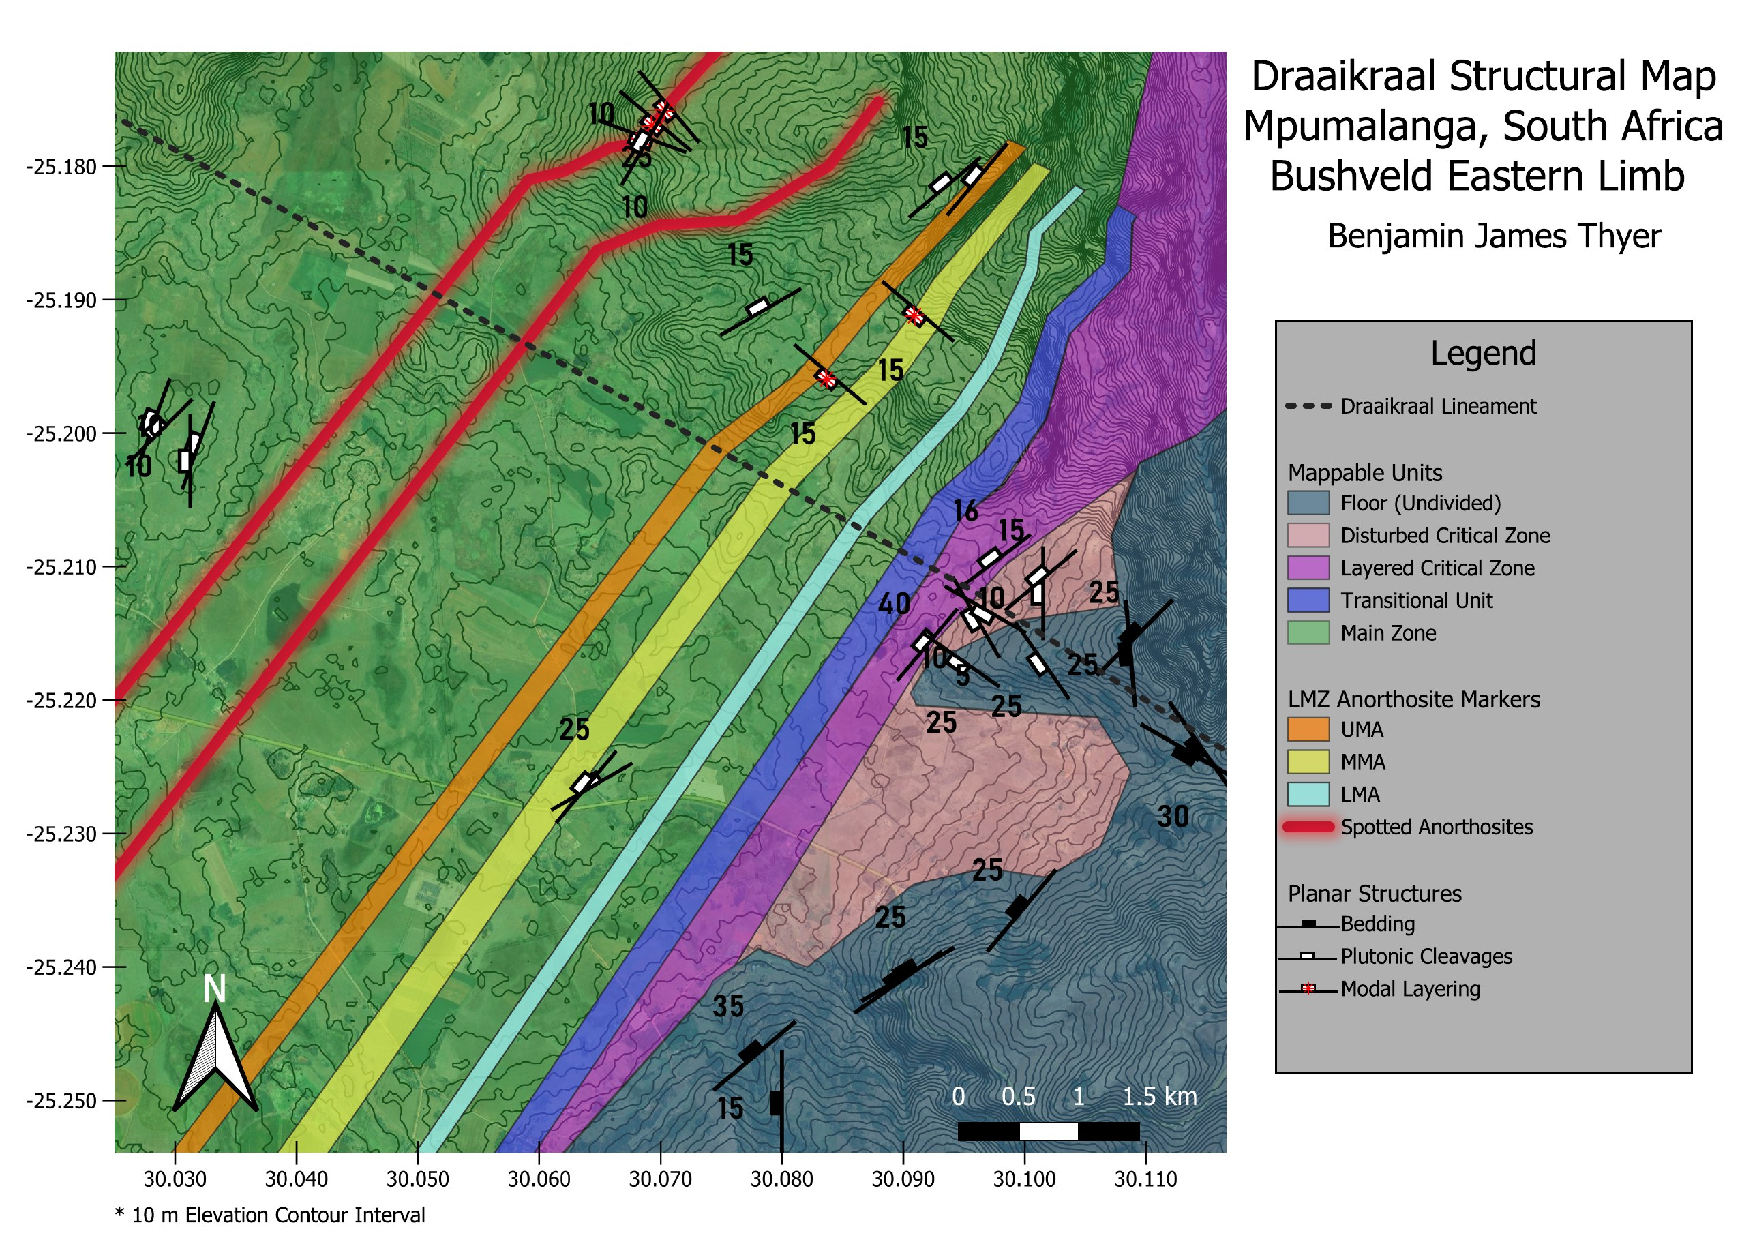
\includegraphics[width=\textwidth]{structural_map.pdf}
  \caption{Topographic and geological map of the Draaikraal field area, compiled from
    Molyneux et al. (2008) with the Upper Critical Zone contact to the south added
    following Van der Merwe (2007). The Draaikraal Lineament (dashed line) separates
    topographically resistant Main Zone gabbronorites to the north from the recessive
    Main Zone in the agricultural valley to the south, without offsetting the high
    ridges of resistant strata (gray box).}
  \label{fig:ch5-topo-map}
\end{figure}

\section{Field Observations}
\label{sec:ch5-field-observations}
% NOTE: this \section break is editorial, added when reorganizing this chapter
% from the raw field-report text (Chapter5/Workspace/Draaikraal 2023 BJT.tex) --
% the original report had no heading here and simply continued straight from
% the Geological Background literature review into "Lithologic Descriptions"
% (see CHANGES_JOURNAL.md-style note in chapter5.tex). It groups the two
% following subsections -- site-specific Lithologic Descriptions and
% Structural Observations -- as the chapter's field-observations material,
% mirroring ChapterA/chapterA.tex's own Field Observations section and
% Chapters 1-3's Methods/Results-style organization. No sentence of the
% original text was altered by this insertion.


\subsection{Lithologic Descriptions}
\label{sec:ch5-lithologic-descriptions}

\subsubsection{Eastern Margin}
\label{sec:ch5-eastern-margin}

Much of this study focused on the eastern margin of the Eastern limb of
the Rustenburg Layered Series (RLS) east of Draaikraal. The margin
displays the most unambiguous bedding planes of the study area,
generally dipping 25° to the northwest towards the center of the
Bushveld Complex, except for the Kliprivier Synform, which is detailed
below in the ``Structural Observations'' section. The marginal rocks
within the field area are composed of gabbroic intrusive igneous sills
concordantly intercalated with variably metamorphosed, melted, or
otherwise devolatilized Transvaal sediments of the Steenkampsberg and
Houtenbek formations. Occasionally, melting and/or reactive porous flow
of melts through sedimentary layers remineralizes sedimentary layers
with igneous mineralogy and texture (photos 35, 51, and 52). Concordant
sills of marginal zone magmas and packages of sediment range in
thickness from 10 to 100s of meters thick, and can be found mutually
interbedded at least a kilometer from the margin of the RLS. Here, the
marginal rocks are divided into three units: ``Rz'', the fine-grained
Marginal Zone gabbroic sills/magmas; ``Qz'', relatively undisturbed
Houtenbek quartzite; and ``ScP'', hornfelsed metapelites, marbles, and
quartzites with related igneous/hydrothermal pegmatites.

\subsubsection{Rz -- Fine grained gabbro}
\label{sec:ch5-unit-rz}

The Marginal Zone gabbroic sills are commonly fine grained (\textless1
mm), but locally are coarser with some grains up to 2 mm in the
groundmass. Unlike much of the plutonic RLS, the Marginal Zone is not
visibly modally layered. Marginal Zone magmas within a meter of
Steenkampsberg Quartzite often contain conspicuous evidence of silicic
contamination: although they retain an igneous texture, the color
significantly lightens and the rocks become much harder and less
magnetic approaching the contacts with Steenkampsberg Quartzite. Aside
from these immediate contacts, the Marginal Zone gabbro is always
magnetic. The Marginal Zone contains more pyroxene (distinguishing
clinopyroxene and orthopyroxene is difficult with such small crystals)
than plagioclase with variable magnetite, sometimes up to 10\%, and
minor phlogopite. The heavy, fine fraction of mineral separates from one
sample was briefly studied under optical microscope to identify trace
phases, which include apatite, zircon, sulfides, and euhedral chromite.

The Marginal Zone magmas contain igneous xenoliths and are rich in
paleo-vertical, across-strike features that likely record rising,
buoyant fluid/magma. Perfect planar resistance banding (photo 95) is the
most common structure in the fine grained Marginal Zone and is nearly
ubiquitous within the unit. Though the resistance bands have seemingly
random strikes, they most often are steeply dipping and may represent
fluid conduits along brittle fractures within the Marginal Zone.

In previous works, isolated meta-sedimentary xenoliths (Buick et al.,
2000) were emphasized, but in this study, meta-sedimentary rocks were
never found as minor xenoliths within magnetic marginal sills, but
rather as continuous, concordant strata (photos 42, 70, 71) or as
locally abundant disaggregated broken strata cemented within a pink,
evolved diatexite (photo 100), both designated as a distinct unit: ScP.

The magnetic sills of the Marginal Zone (Rz) did include enclaves of
coarse-grained leucogabbronorite, mottled anorthosite or pyroxenite
(photos 2,4,6,96). The anorthosite-rich enclaves are rounded, 6-10 cm
along their longest dimension, and are imbricated to be preferentially
lying flat paleohorizontally within the Marginal Zone, suggesting they
were weathered/eroded by reaction and/or mechanical transport through
Marginal Zone magma. Pyroxenitic enclaves are also often spherical
(photos 4, 96) and may be related to the formation of the pyroxenite
``Tennis Ball Marker'' (TBM) of the Main and Critical Zones, described
further in the discussion. These plagioclase-rich igneous xenoliths
contain large (\textless3 cm) optically continuous oikocrystic augite
that enclose blocky plagioclase (\textless5 mm).

More commonly observed within the magnetic Marginal Zone sills east of
Draaikraal are paleovertical structures that suggest buoyant upwelling
of fluids and melts sourced from the hornfelsized sedimentary rocks.
These structures included sheared, visco-elastically deformed lenses of
thin pegmatites, including anorthosite (photo 6), magnetite gabbros
(photo 60, sheared gabbro \textasciitilde{} 10 x 3 cm), and evolved
quartz-biotite pegmatites (photo 67: 1x3 cm). In addition to homogeneous
pegmatites, the Marginal Zone gabbros host paleovertical invasions of
anastomosing anorthosite derived from anatexis of underlying
metasedimentary rocks (photos 6, 97). These leucosome intrusions
occasionally carry blocks of meta-sedimentary paleosome or brecciate and
enclose the Marginal Zone gabbronoritic host rock itself (photo 98).

Near the contact with the migmatite, differential weathering sometimes
reveals proud, thin, pinched ovate paleovertical structures (5x1 cm
scale) on weathered faces of Marginal Zone norite that are otherwise
invisible on a fresh rock face {[}photo 40{]}.

The contact between the layered series (Critical and Main Zones) and the
Marginal Zone is likely a fault contact at the Kliprivier Synform, but
elsewhere appears gradational, requiring a somewhat arbitrary
categorization. Since the Lower Main and Upper Critical Zones are
non-magnetic and marginal zone rocks are magnetic, I chose
field-detectable magnetism as the simple discriminant to distinguish
marginal rocks from the massive main and critical zones of the RLS,
though these main and critical zone rocks near the margin may inherit
some features typical of the marginal zone, such a resistance banding.
Fine-grained Marginal Zone gabbros are mapped up to 120 meters below the
Merensky Reef stratigraphically.

\subsubsection{Qz -- Houtenbek Quartzite}
\label{sec:ch5-unit-qz}

The Houtenbek quartzite dips concordantly with marginal zone sills and
migmatized sedimentary rocks towards the center of the Bushveld, here
dipping about 25° to the northwest. Even within meters of a contact with
Marginal Zone sills (Rz), the quartzite often retains a clastic
sedimentary texture and possibly could be considered a proper
clast-dominant quartzose sandstone with well-sorted and well-rounded
coarse quartz grains \textasciitilde1 mm in diameter with no other
mineral visible. While there is little structure visible internally
because of the purity of the quartzite, the bedding planes occasionally
reveal conspicuous asymmetric ripple structures {[}photos 2, 68{]}
\textless1 cm in height. One in-place ripple structure suggests a
paleoflow direction towards the South-Southwest. Some quartzites are
hornfelsized: recrystallized into an interlocking crystalline texture
with large, irregular, angular, coarse grains \textless2 cm across. Many
quartzites with preserved clastic textures near the margin of the RLS
are stained bright red within rocks' unweathered interior. This staining
is hypothesized to be derived from mobilized Fe-rich fluids percolating
along grain boundaries, probably caused by heat and/or fluid circulation
related to the emplacement of the RLS. Steenkampberg Quartzite is mapped
up to 140 meters below the Merensky Reef stratigraphically.

\subsubsection{ScP -- Houtenbek Hornfels, Migmatites, Pegmatites}
\label{sec:ch5-unit-scp}

In addition to quartzite, the Houtenbek formation contains carbonate and
pelitic horizons (Button, 1976). At the margin East of Draaikraal, there
is a 60 m thick package of melted and metamorphosed sediment containing
stratiform pegmatites with variable mineralogy. Hornfelsized sediments
come in two main varieties near Draaikraal: pink, diatexite-supported
breccias {[}photo 100{]} or dark, high-grade schists {[}photo 29{]} with
thin but conspicuous navy, gray, white, tan, and pink bands of
relatively mafic and felsic minerals have been recrystallized and no
longer bear clastic textures except for thin seams of clast-dominated
quartzite in a low-fraction glassy biotite-rich matrix {[}photo 35,
large light seam is \textasciitilde4 cm thick{]}. This unit is rarely
magnetic and most often is visible as continuous, concordant strata
{[}photo 42{]}. Even when highly brecciated, this unit can be followed
along the strike of the quartzites and Marginal Zone, implying that the
sediments were not incorporated into Marginal Magmas, but that they
rather were melted and devolatilized in-situ due to heating from the
emplacement of adjacent marginal sills. Fluids and melts produced in
this process are visible as a wide variety of stratiform pegmatites and
skarns with undulating erosive contacts within comparatively planar
meta-sediments {[}photo 30: feldspar/wollastonite(?) + Amphibole skarn;
photo 69: Magnesite, quartz pegmatite with minor siderite{]} and as
pockets following fluid flow pipes and void spaces that are accommodated
by the host strata through ductile deformation {[}photo 37, 38:
Orthopyroxene and quartz pegmatite{]}. Hornfels in the field area are
mapped up to 190 meters below the Merensky Reef stratigraphically.

\subsubsection{The Rustenburg Layered Series (RLS)}
\label{sec:ch5-rls-units}

The Rustenburg Layered Series is the World's largest individual igneous
intrusion (Cawthorn, 2015; Latypov, 2022) and is subdivided into the
Lower Zone, Critical Zone, Main Zone, and Upper Zone. In this study, RLS
rocks of the lower Main zone, Transitional Zone, and upper Critical zone
are mapped. The rocks of the Marginal Zone (Rz) are not layered, nor
considered here to be a part of the RLS on a textural basis. Marginal
zone rocks weather distinctly from the plutonic RLS phase with abundant,
sharp, \textasciitilde3 cm-scale potholes and generally are more
textured and rough {[}photo 36{]} on a weathered surface than RLS rocks,
which weather spheroidally and proudly {[}photos 8, 11: ``porphyritic''
gabbronorite{]}. Xenolith blocks of Marginal Zone norites bearing their
distinctive resistance banding are found in both the Critical and the
Main zones {[}Critical Zone: photo 76; Main Zone: 91{]}, though each
xenolith sighting within the Main Zone is proximal to a mottled or
spotted anorthosite layer. These xenoliths are variably annealed,
recrystallized, and even ductily deformed {[}Critical Zone: photo 77;
Main Zone: 84{]}.

The RLS is famous for its distinctive and numerous laterally continuous
stratiform marker horizons, sometimes stretching on a 100-km scale
(Cawthorn, 2015), which include the Critical Zone chromitite cycles,
Merensky and Bastard pegmatoid reefs, three mottled anorthosite packages
in the lower Main Zone, the Pyroxenite Marker of the upper Main Zone,
and the magnetitite cycles of the Upper Zone. In this study, I observe
and describe the three lower Main Zone magnetic mottled anorthosites
{[}photos 49, 53, 86, 93, 105, 106, 108, 111{]}, the magnetic chromitite
UG2 {[}photos 65, 66{]}, and a non-magnetic upper Critical Zone mottled
anorthosite that is probably a part of the Merensky Reef footwall
{[}photo 81{]}, and several packages of xenolith-bearing modally layered
gabbronoritites and spotted anorthosites within the Main Zone (photos ).
These laterally continuous reefs are mapped and described separately
from the bulk cumulate rocks of the RLS.

\subsubsection{Cz: Critical Zone}
\label{sec:ch5-zone-cz}

The Critical Zone was previously mapped to pinch out due East of
Draaikraal (shown in the compilation of Molyneux et al., 2008), however
many now recognize that a thin layer of the upper Critical Zone persists
much further south towards Tontledoos (Van De Merwe, 2007). In this
study, diagnostic Critical Zone lithologies were only observed north of
the Kliprivier syncline, where typical finely modally layered norites
and anorthosites are well-exposed (photos 64 and 80), as well as the UG2
chromitite. The Critical Zone above the Kliprivier Syncline dips
\textasciitilde15° to the northwest similarly to the majority of the
Main and Marginal Zone rocks in the field area, but gradually rotates to
a southwestern dip as it approaches the contact with the rotated block
of metasediments and gabbronorite sills of the Kliprivier Synform. It is
essential to note that some rotated Critical Zone rocks are structurally
beneath the large, rotated package of intruded metasediments (Rz + Qz +
ScP) in the area of the Kliprivier Synform, meaning that this package of
country rock is not only serving as the floor for RLS rocks to the west,
but is also (at least locally) a roof for Critical Zone rocks below the
level of the UG2.

\subparagraph{Dcg: Disturbed Gabbronorite}
\label{sec:ch5-unit-dcg}

This lithology is restricted to the immediate area of the Kliprivier
synform. Disturbed Gabbronorites are coarse-grained, even pegmatoidal
(photo 62), with feldspars and pyroxenes up to 3 cms long. This unit was
named in response to Van Der Merwe (2007), who said that the
``structural change {[}of the Klipriver Synform{]} is reflected in the
Bushveld rocks, which become highly disturbed and fragmented''.
Disturbed Gabbronorites are most recognizable for their abundance of
blobby autoliths of anothosite (photo 61) and pyroxenite (photos 70 and
72). While it exhibits abundant examples of modal separation, they are
never remotely planar, unlike the majority of the RLS. I interpret this
unit to be formed by synmagmatic deformation of nascent layered upper
Critical Zone mushes during the formation of the Kliprivier Synform,
effectively breaking up and redistributing the nascent layering into
many blobs.

This lithology is most often non-magnetic, but a few specimens were
magnetic. Besides the mottled anorthosites of the Main Zone and the
anothosite-hosted chromitite leader of the UG2, no other rocks of the
RLS within the field area are magnetic. Many but not all Disturbed
Gabbronorites are rotated within the Kliprivier synform. Generally, the
Disturbed Gabbronorites are CPX-poor and sulfide-rich with abundant,
euhedral \textless1 cm pyroxenes set in an anorthosite matrix that
effectively isolates the large, euhedral pyroxenes from one another
{[}photo 62{]}. This unit generally becomes more feldspathic as one
moves away from the intruded metasediments of the Kliprivier Syncline
into the Critical Zone. This lithologic unit contains recrystallized and
annealed xenolith blocks {[}photos 74, 75, and 77{]} of fine-grained
Marginal Zone gabbros (Rz) as well as coarse-grained pockets containing
very large (\textless{} 5cm) oikocrystic pyroxene {[}photo 73{]} and
large clusters of pyroxene often rimmed by thick anorthosite halos
{[}photo 72{]}. Disturbed Gabbronorite is mapped between 120-145 meters
below the Merensky Reef stratigraphically, around the level of the UG1
in core logs (Van Der Merwe, 2007). Van Der Merwe (2007) and Latypov et
al. (2022) report isolated patches of massive chromite here, but I did
not see any.

\subparagraph{UG2: Upper Group 2 Chromitite}
\label{sec:ch5-unit-ug2}

Near the top of the upper Critical Zone in the extreme northern portion
of Kliprivier farm, there is a small but high-quality exposure of
chromitite (\textgreater30 cm thick). The bulk of the exposure is a
melanocratic, non-magnetic, anorthositic chormite, which is modally
\textasciitilde50\% \textless1mm euhedral chromite set within a fine
matrix of \textless1 mm plagioclase (photo 66). Structurally above this
massive layer are some thin (\textless1 cm thick) chromitite leaders
hosted within bright white mottled anorthosite (photo 65). Both layers
contain amoeboid oikocrystic pyroxene-olivine mottles (\textless2cm).
The mafic silicate mottles and anorthosite matrix seem to have
crystalized within the interstices of a preexisting framework of a
continuous chromite crystal slurry {[}photos 65, 66{]}, (see Voordouw et
al., 2009 and Mukherjee et al., 2017 for similar interpretations). The
massive melanocratic layer includes pure (relatively chromite-free)
white anorthosite blocks (\textless4x15 cm) that are lying flat and
dipping west towards the center of the Bushveld complex. These pure
anorthosite blocks contain thin chromitite stringers that together have
been ductilely deformed, and a thin (\textasciitilde1 mm) white seam of
pure, apparently undeformed anorthosite forms a plane bounding the top
of some of these blocks, also dipping to the west.

The anastamosing chromite leaders within the overlying mottled
anorthosite are sometimes highly magnetic and are a much deeper,
vitreous black: appearing under hand lens to be \textgreater80\% modally
chromite/magnetite {[}photo 65{]}.

This chromitite package is interpreted as UG2 for a few reasons. First,
although the anastomosing chromite leader resembles the UG1 stringers,
the leader is structurally above the massive chromitite, whereas the UG1
stringers are recognized below the massive chromitite (Voordouw et al.,
2009 and Mukherjee et al., 2017). The UG2 is known to have several small
``leaders'' a small distance above the main seam (Maier and Barners,
2024). Second, the magnetic chromitite within the leader bears
explaining. One heterogeneous magnetic chromitite at the top of the UG2
with discrete magnetic and non-magnetic bands was described by J.J.
Frankel (1942), 20-30 km to the north of Kliprivier at Tweefontein.
Third, a rock at this location was also mapped as the UG2 by Harmer and
Shaper (1985: Fig. 4) and Van De Merwe (2007: Fig. 3), who also
identified the UG2 and closely overlying mottled anorthosites in drill
cores of the area using PGE grades. Van Der Merwe (2007) also reports
that the UG2 at Kliprivier is unusually enriched in iron, which may
explain the magnetism of the leader. The UG2 is 86 meters below the
Merensky Reef in the direct vicinity of the Kliprivier Synform (Borehole
3: Van Der Merwe, 2007).

\subparagraph{Ln: Layered Norite:}
\label{sec:ch5-unit-ln}

Spectacular outcrops of modally layered norites within the upper
Critical Zone are observed within the field area at Kliprivier around
and above the stratigraphic level of the UG2 chromitite (photos 64 and
80), at stratigraphic heights from 100 to 50 meters below the Merensky
Reef. Modal layering is pronounced, with pyroxenite-rich layers being
separated by near-pure centimetric anorthosite bands. This layering is
undulose and irregular.

\subparagraph{Px: Pyroxenite}
\label{sec:ch5-unit-px}

This refers to rocks predominantly composed of pyroxenes. Pyroxenites
are rare in the field area. There was one coarse-grained sulfide-bearing
feldspathic pyroxenite horizon in the Critical Zone just below the UG2
(photo 78) as well as a pyroxenite layer just below a mottled
anorthosite layer in the UMA in the lower Main Zone (photos 53-54).

\subsubsection{Tz: Transitional Zone}
\label{sec:ch5-zone-tz}

There is no perfect division for the Main and Critical zones. Moving
upsection from the Critical Zone into the Main Zone, Cr2O3 concentration
within OPX abundance decreases, Strontium isotopes become more
radiogenic, and cumulus clinopyroxene becomes important--- but these
changes occur at different stratigraphic heights within the transition
zone (Cawthorn, 2015) between the Merensky Reef and Giant Mottled
Anorthosite (or above). Within the literature, the bottom of the Main
Zone is considered to be above the Giant Mottled Anorthosite at the top
of the Bastard unit, and the Merensky reef is taken to be the top of the
Upper Critical Zone. (Cawthorn, 2015; Mitchell and Manthree, 2002; Van
de Merwe, 2007). The Bastard and Merensky pyroxenites and Giant Mottled
Anorthosite were never observed in the field area, but a
\textasciitilde50 cm thick mottled anorthosite {[}photo 81{]} was
observed \textasciitilde50 meters upsection from the UG2 with only
finely layered norite {[}photo 80{]} and porphyritic gabbronorite
outcropping between the UG2 and the mottled anorthosite. Since Van De
Merwe (2007) reports in core logs that the Merensky Reef is 86 meters
above the UG2 on Kliprivier and Latypov et al. (2022) observe unusual
pyroxenites just above this mottled anorthosite, this anorthosite layer
is interpreted to be a part of the footwall to the Merensky Reef, and
the pyroxenites described in Latypov et al., 2022 are interpreted to be
the Merensky Pyroxenite.

\subparagraph{Pg: Porphyritic Gabbronorite}
\label{sec:ch5-unit-pg}

The ``Pophyritic Norite'' is a well-recognized marker of the lower Main
Zone, with large, rounded pyroxene phenocrysts set in a white,
feldspar-rich matrix, used often in mining to locate the Merensky Reef
(SACS, 1980; Von Gruenewaldt et al., 1985). I observe a general textural
similarity in lower Main Zone Gabbronorites with the unlayered upper
Critical Zone gabbronorites below the Merensky Reef (photos 10, 79).
These gabbronorites are distinct from the dark and homogeneous
gabbronorites that compose the majority of the Main Zone (Hg). The
porphyritic gabbronoite contains large (\textasciitilde\textless{} 1cm),
equant pyroxenes set in a leuconoritic matrix that is predominantly
plagioclase with small spots of interstitial orthopyroxene. I refer here
to them collectively as the ``porphyritic gabbronorite'' because I see
cumulus clinopyroxene present throughout, becoming more modally abundant
upsection until about half of the cumulus pyroxenes are CPX near the
Lower Mottled Anorthosite (LMA). Generally, cumulus CPX is present in
the Main Zone and absent from the Critical Zone (Cawthorn, 2015).
However, some cumulus CPX has been reported at the top of the Critical
Zone (Cameron, 1982; SACS, 1980).

The rocks of this unit have well developed cleavage {[}photo 63{]};
however, they are not visibly layered. I located porphyritic
gabbronorite south of the Kliprivier Synform at the beginning of the
second field day and assumed it was Main Zone given the cumulus CPX I
saw, but now I believe that the porphyritic gabbronorite occurs in the
upper Critical Zone through the Transition Zone and into the lower Main
Zone in the vicinity of Draaikraal. The Porphyritic Gabbronorite in this
field area hosts spherical pyroxenite tennisballs (photos 10, 79), in
the same locations as mapped by Harmer and Sharp (1985) and Mitchell and
Scoon (2023). Porphyritic Gabbronorite is mapped in the Critical and
Main Zones 480 meters below the Merensky Reef to 380 meters above,
stratigraphically.

\subsubsection{Mz: Main Zone}
\label{sec:ch5-zone-mz}

The Main Zone is the most volumetrically significant portion of the RLS:
as thick as 5 km (Latypov et al., 2022). The Main Zone stratigraphy is
(in general) relatively featureless aside from three prominent mottled
anorthosite packages in the lower Main Zone and the Pyroxenite Marker at
the upper Main Zone, which was not studied in this work. Mottled
anorthosites and associated strongly modally layered sequences are
mapped and described here in order to study the effect of the Kliprivier
Synform and Draaikraal lineament on the stratigraphy, as these unique
layers can be traced great distances through the Lower Main Zone
(Latypov et al., 2022).

\subparagraph{Hg: Homogeneous Gabbronorite:}
\label{sec:ch5-unit-hg}

The massive Homogeneous Gabbronorite of the Main Zone varies slightly in
color due to variations in the modal abundance of pyroxenes and
plagioclase, though these variations are subtle and continuous on a
scale of 10s of meters. There is no obvious fabric visible in outcrops
or hand samples of these massive rocks, although I was shown a polished
core of upper Main Zone gabbronorite from a dimension stone mine east of
Roossenekal that obviously displayed a fabric where crystals
preferentially were aligned with the gravitational plane. Stonemasons
favor this rock for building, but are careful to allow only faces cut
against this fabric to outwardly show for aesthetics and durability.
Homogeneous Gabbronorite (Hg) begins about 450 meters above the Merensky
Reef and continues upsection stratigraphically through the Pyroxenite
Marker (SACS, 1980; Von Gruenewaldt et al., 1985).

\subparagraph{(L/M/U)MA: (Lower/Middle/Upper) Mottled Anorthosites}
\label{sec:ch5-unit-lmuma}

Mottled Anorthosites are enigmatic igneous rocks composed of a nearly
pure, white anorthosite matrix containing (often quite large: \textless5
cm) mossy green ``mottles'' of oikocrystic pyroxene +/- olivine that
enclose abundant plagioclase. In the RLS they are found in large
stratiform horizons interpreted to be continuous across the majority of
the Main Zone in the Bushveld (\textgreater100 of kilometers: Latypov,
2022). The lower Main Zone near Draaikraal contains 3 large mottled
anorthosite packages. These mottled anorthosites are magnetic and
notably contain rare large (\textless{} 2mm) grains of magnetite within
the mottles. They are found in association with larger packages of
distinct but non-magnetic anomalous lithologies. The associated unusual
rocks include: 1) fine green gabbronorites with blebby, anhedral
phenocrystic (\textless2 cm) clinopyroxene (lithologic code Fgog:
Fine-grained oikocrystic gabbronorite) associated with the UMA; 2)
feature-rich, coarse pyroxenites (lithologic code: Px, {[}photos 53,
54{]}) and 3) blobby pyroxenitic gabbronorites (lithologic code Bap:
Blobby anorthosite-pyroxenite) that include deformed, irregular,
decimeter scale blobby pyroxene agglomerations within an anorthositic
matrix that are interpreted here to be recrystallized blocks {[}photos
104, 108{]}. Sometimes these blobby anorthosite-pyroxenites exhibit
modal layering of coarse (\textless2 cm) pyroxene oikocrysts {[}photo
105{]} within anorthosite. The mottled anorthosites and their associated
pyroxenites and blobby gabbronorites have undulating, nonplanar contacts
with one another {[}photo 49{]} and with the underlying common
gabbronorites {[}photos 107, 103{]}. Sometimes these contacts may be
drastically discordant from the local strike and dip. In photo 106, the
mottled anorthosite - gabbronorite contact is dipping \textasciitilde70°
to the East towards the margin of the chamber: a much steeper dip and
opposite strike than observed in the leucogabbronorites of the immediate
vicinity. Occasional 3D exposure of the anorthosite-gabbronorite contact
allowed me to measure the contact rotating 90+ degrees in this outcrop
within meters (photo 107). It is unclear if these undulating contacts
are evidence for discordance of the mottled anorthosites, since in other
places the contact appears concordant {[}photo 110{]}, and local
apparent discordance could be the result of thermal erosion of the
cumulate pile by overlying magmas (Roberts et al., 2007).

It is important to note that one outcrop of mottled anorthosite clearly
showed disagreeing cleavage and planar modal layering, with modal layers
dipping 50° more eastwardly than the rock cleavage {[}photo 115,
annotated below in figure 1{]}. This suggests that cleavage and modal
layering are formed by distinct processes that may have occurred at
different times, with modal layering likely predating the formation of
rock-cleavage (see Structural Observations section for more details).

In this study, all three lower Main Zone anorthosites described by
Latypov et al. (2022) and mapped by Van Der Merwe (2007) were located
within the low-lying valley south of the Draaikraal Lineament at
stratigraphic heights between 200 and 600 meters above the level of the
Merensky Reef. The Upper and Middle ``mottled'' anorthosites in the
mountains to the north reported by Latypov et al., 2022 were located on
this study, but are visually quite distinct and occupy much higher
stratigaphic heights (\textgreater1000 meters) argued here to be
distinct units that stratigraphically overly the thick, massive mottled
anorthosites in the valley to the south (see the Discussion of this
work). Von Gruenewaldt et al. (1985) report multiple subordinate
anorthositic layers near and at the boundary of the Main Zone subzone A
and B much higher above the level of the Main Mottled Anorthosite. Those
higher anorthosites are referred to here as spotted anorthosites (SA) to
reflect their distinct texture. Though this particular contested
correlation by Latypov et al. (2022) is of minor significance to the
overall argument put forward in their work, it is essential evidence to
understand the origin and significance of the Draaikraal Lineament as
the surface expression of a synmagmatic monocline formed by laccolithic
deformation during the intrusion of much of the Critical Zone.

\subparagraph{SA: Spotted Anorthosites}
\label{sec:ch5-unit-sa}

North of the Draaikraal Lineament where exposure is better, two packages
of anorthosites were found in the lower Main Zone. These anorthosites
are somewhat distinct from the common, unlayered gabbronorites of the
Main Zone, but anorthositic beds are significantly smaller (\textless1 m
thick) and altogether less visually striking than the Mottled
Anorthosites (MA) unit described above. The spotted anorthosites are
non-magnetic and bear \textless1 cm spots of equant pyroxenes composing
\textless20\% of the rock by volume {[}photos 86, 87{]} that sometimes
contain recrystallized pyroxenite-gabbronorite blocks {[}photo 111{]}.
The Spotted Anorthosites are strongly associated with much thicker
(\textless10 m) packages of planar, finely layered gabbronorites that
are unusual within the Main Zone and are more reminiscent of the
Critical Zone {[}photos 85, 112{]}. These modally layered sections also
include xenoliths {[}photos 91, 84{]}, which were only observed within
the Main Zone in these modally layered packages. These Spotted
Anorthosite packages are argued here to be distinct and
stratigraphically above the remarkable and prominent Mottled
Anorthosites described above. Two or three packages of Spotted
Anorthosites (often including thick layers of Layered Gabbronorite) are
interpreted here at stratigraphic heights 700-1050 meters above the
Merensky Reef. More packages may exist, although they are unlikely to be
exposed to the south of the Draaikraal Lineament.

\subparagraph{Lg: Layered Gabbronorite}
\label{sec:ch5-unit-lg}

Modal layering is generally less common in the Main Zone than the
underlying Critical Zone, and in outcrop it is comparatively
understated. Whereas the Ln (Layered Norite) unit of the Critical Zone
contains vivid, centimeter-scale, near-monomineralic anorthositic bands,
the modal layering in the Main Zone gabbronorites is millimeter-scale,
represented by subtle differences in cumulus grain size and modal
proportions, and the contacts between layers are planar (photos 85 and
112). The Layered Gabbronorites are associated with Mottled Anorthosites
(MA) or Spotted Anorthosites (SA). When Layered Gabbronorites (Lg) are
observed in the same outcrops as Mottled or Spotted Anorthosites, the
locality is assigned to be Mottled or Spotted Anorthosite. Layered
Gabbronorites are mapped here at stratigraphic heights between 400 and
1050 feet in association with Mottled and Spotted Anorthosites.

\begin{figure}[htbp]
  \centering
  \todo{Insert annotated field Photo 115 here (cleavage and modal layering in a
    Mottled Anorthosite outcrop) -- source image not yet organized into
    Chapter5/Figures/source/; original reference was to a pandoc-extracted
    media/image1.jpg that was never carried over with the raw report text.}
  \caption{Cleavage and modal layering forming distinct planes in a Mottled
    Anorthosite outcrop (annotated Photo 115).}
  \label{fig:ch5-ma-cleavage-photo}
\end{figure}

\subsubsection{Post Bushveld Rocks}
\label{sec:ch5-post-bushveld-rocks}

In the valley surrounding Draaikraal, alluvium primarily is composed of
well-rounded quartzite cobbles (\textasciitilde10 cm) and ironstone
laterites. The ironstone laterites are commonly found as both float in
alluvium and as in-place outcrops. Bushveld mafic rocks are rare in
alluvium, probably due to their relative susceptibility to chemical
weathering on Earth's surface. Quartzite was substantially dominant over
RLS mafic rocks in alluvium even 8 km away from the nearest known
quartzite source within the RLS, leading Dr. James Roberts and I
originally to suspect that there were closer quartzite sources; however
we were unable to identify quartzite sources west of Draaikraal. It is
likely instead that the creeks which source their headwaters from the
Houtenbek and Steenkampsberg quartzite highlands to the East and flow
past Draaikraal to the West, transported and rounded these cobbles,
which are much more stable on the surface than the RLS rocks, eventually
coming to dominate the regional alluvium.

\subparagraph{IS: Ironstone Laterites}
\label{sec:ch5-unit-is}

Ironstone laterites are common throughout the relatively low and flat
valley surrounding Draaikraal. They are somewhat weakly-consolidated and
highly porous non-magnetic amalgamations of \textless1cm iron
concretions composed of 1 mm thick deep black vitreous goethite rims
surrounding pockets of fine-grained yellow limonite matrix. Interspersed
between these concretions are variably rounded medium-coarse
Steenkampsberg quartzite gravels. The goethite nodules and quartz
gravels are cemented by fine grained, red and yellow hematite-limonite
matrix with mm-scale angular, coarse, quartz sand. The existence and
abundance of these ironstone laterites implies that the valley
surrounding Draaikraal is a longstanding, persistent topographical
feature that has existed on geological timescales. They were likely
formed by in-place weathering of RLS rocks, explaining the relative
dearth of RLS material within the valley alluvium.

\subparagraph{Dl: Dolerite Sill:}
\label{sec:ch5-unit-dl}

Post-Bushveld Dolerite sills are mapped throughout the field area
(Merwe, 2007; Molyneux, 2008), and one such discordant sill was observed
at the levels of the UMA and MMA north of the Draaikraal Lineament
within the field area (photo 89). Despite being younger than the
surrounding RLS, the sill is significantly more weathered, likely
because of extensive blocky fracturing hypothesized to result from rapid
contraction during cooling. The dolerite is moderately magnetic.

\subsubsection{Stratigraphic Column Analytical
Methods}\label{sec:ch5-stratigraphic-column-methods}

The field data of this study north of the Kliprivier Monocline is
projected onto a stratigraphic column following the assumption that all
rocks in the field area north of the Kliprivier Monocline follow
Stenno's Law of Original Horizontality and were only uniformly deformed
by tilting due to isostatic flexure towards the center of the RLS after
emplacement, so that all regional bedding and structures are currently
dipping 15 degrees to the northeast relative to their original
orientations. Geolocated field data is projected onto a line above the
Kliprivier Monocline designed to be orthogonal to the regional strike
(trending 301.79 degrees: W-NW) using the `Snap Geometries to Layer' in
the `Vector Geometry' Processing Toolbox in QGIS, with a tolerance of 1
degree set to ``prefer closest point''. Distances from an arbitrary
point along this line stratigraphically below all points were calculated
using the ``Distance Matrix'' function in the ``Vector Analysis''
Processing Toolbox. A correction was added to these lateral distances to
account for elevation, calculated as the product of the elevation
differential and the tangent of the regional dip, assumed to be 15°. The
column heights are normalized to the height of the UG2, which in turn is
normalized to the height of the Merensky Reef, determined to be 86
meters above the UG2 stratigraphically within the Kliprivier Synform
(Merwe, 2007). Note that no changes in strike and dip are considered,
although the dip of the Main Zone likely shallows and rotates to be
roughly due east further from the margin of the intrusion. The
stratigraphy calculated here was optimized for discriminating units
within the upper Critical and lower Main zones. Therefore, the
stratigraphic heights presented here for the Homogeneous Gabbronite
lithology are likely overestimated. The interpreted schematic
stratigraphic column for the region is graphically presented in figure
5.

\subsection{Structural Observations}
\label{sec:ch5-structural-observations}

\subsubsection{Kliprivier Synform}
\label{sec:ch5-kliprivier-synform}

The most interesting large-scale structure in the mapping area is a
rotated package of disturbed, pegmatoidal upper Critical Zone
pyroxenites and gabbronorites {[}photos 61,62, 72-78{]}, well-cleaved
leuconorite layers {[}photo 63{]}, quartzites {[}photos 28 and 124{]},
migmatized/hornfelsed argillites and calc-silicate layers {[}photos 29,
30, and 125{]}, and marginal sills {[}photo 57{]} in the northern
portion of Kliprivier Farm. The structure is remarkable because it
apparently displaces a marginal package of metasediments and
fine-grained sills over 1.25 kilometers into the plutonic RLS. This
structure is described accurately but qualitatively by Van Der Merwe
(2007), who investigated the area to assess its platinum resource
potential. Van Der Merwe (2007) refers to this feature the ``Kliprivier
Syncline'', though it is not clear if he is naming the structure or it
was named elsewhere. A displaced quartzite layer within the structure
was also observed during the field mapping of the Main Zone mottled
anorthosites by Latypov et al. (2022) and is described in their
supplementary information as a ``Large Quartzite Xenolith?''.

The structure is referred to here instead as the ``Kliprivier Synform''
to recognize that it is not yet well understood. For instance, no
previous work to date has correlated marginal magmas and country rocks
from the two limbs of the putative syncline to demonstrate that they are
the same and that the structure is indeed a fold and not another
structure, such as a laccolithically deformed roof remnant of an RLS
subchamber or a package of floor rocks entrained in a rising magma. The
map presented here offers additional details that elucidate the nature
of this structure. Below, a series of observations of the Kliprivier
Synform is presented:

\begin{enumerate}
\def\labelenumi{\arabic{enumi}.}
\item
  To the north of the structure, there is a continuous, 90° gradual
  change in strike moving from finely-banded noritic Critical Zone,
  which strikes southwest and dips northwest like the majority of the
  mapped lithologies east of Draaikraal, to a southeastern strike
  dipping southwest. This gradual change in structure is accompanied by
  lithologic changes in the Critical Zone: Near and at the deformed
  areas, grain-size increases (photo 61) and stratiform modal layering
  ceases and is replaced by a heterogeneous rock with abundant
  fine-grained Marginal Zone xenoliths, anorthosite autoliths (photo 62)
  and irregular clumps of pyroxene surrounded by anorthosite (photos
  72-77). I have mapped these lithologies as ``Disturbed Gabbronorite''
  (Lithologic code: Dcg).
\item
  To the south, there is little exposure and no structural data could be
  gathered to pinpoint the reversal of the structure back to the common
  northwestern dip. However, outcrops constrain the contact between the
  Marginal Zone magmas and the porphyritic gabbronorite of the upper
  Critical Zone to occur within 10 meters. The ``disturbed'' lithologies
  of the Marginal/Critical zones present on the north side of the
  synform are not present on the south side. Van De Merwe (2007)
  interprets faulting with downthrows to the south at this contact;
  however, Van De Merwe (2007) does not map any vertical displacement of
  marker beds such as the UG2 chromitite at this fault.
\item
  Stratigraphically higher plutonic rocks are undeformed, suggesting
  that they were intruded and crystallized after the deformation forming
  the Kliprivier Synform. Interestingly, the western termination of the
  synform as mapped here occurs at or slightly below the level of the
  Merensky Reef, where a significant magma recharge event corresponding
  to the emplacement of the Main Zone is thought to have occurred
  (Seabrook et al, 2005; Cameron, 1982).
\item
  Displaced plutonic rocks to the north are stratigraphically below the
  quartzites and Marginal Zone sills, meaning that the section of sills
  and sediments serve as a roof to the RLS to north.
\item
  Within this study, there is one strike and dip measurement immediately
  to the West of the structure, that is striking SW like the majority of
  the field area but is dipping more steeply than other rocks in the
  region. Latypov et al. (2022) also report an unusually steeply dipping
  plutonic rock along strike.
\item
  To the east, the structure is attached to the floor of the RLS.
  Unfortunately, that area was not mapped in detail and the nature of
  the rotation from the synform's exotic dip to the common dip of the
  marginal series was not observed.
\end{enumerate}

Strike and dip measurements taken from the Kliprivier Synform were
plotted on a stereonet and analyzed using Stereonet 11 (Almendinger et
al., 2012, Cardozo and Almendinger, 2013). Poles to bedding planes of
quartzites, hornfels, mafic sills, and plutonic rocks were calculated
and plotted together in stereonet projection in Figure 3. In Figure 4,
the fold axis is calculated using the poles to the bedding planes. This
calculated fold axis trends roughly W5°N, plunging 15°, similarly to the
Draaikraal Lineament. The axial plane also was calculated, assuming it
bisected the obtuse angle formed by the limbs. The obtuse fold angle
bisector for the axial plane was selected because the rotation within
the fold observed is quite gentle. An acute bisector for the axial plane
would've been better supported if field evidence showed dramatic changes
in dip along the fold, requiring a complete structural overturn that
locally annihilated the original horizontality of the deformed rocks in
addition to steeply dipping rocks intermediate to the two limbs. The
calculated obtuse bisector axial plane strikes W°5N and dips 85°.

The axial plane is similar in orientation to the WNW-ESE trending
Draaikraal Lineament that bounds the topographically high and low Main
Zone rocks. Considering that the Kliprivier Synform also rests upon this
lineament, it is likely that the formation of the Kliprivier Synform is
related to the Draaikraal Lineament.

\todo{Insert Figure 3 (Kliprivier Synform structural map/cross-section),
Figure 4, and Figure 5 (interpreted schematic stratigraphic column referenced in
\S\ref{sec:ch5-stratigraphic-column-methods}) here. Source figures are not yet
organized into Chapter5/Figures/source/.}

\section{Sample and Station Data}
\label{sec:ch5-sample-station-data}

The field data underlying \S\ref{sec:ch5-field-observations} -- GPS-located
stations, stratigraphic heights, interpreted units, and lithologic
descriptions -- are compiled in Table~\ref{tab:ch5-field-stations}.
Structural measurements (strike, dip, and structure type) recorded at a
subset of these and additional dedicated structural stations are compiled
separately in Table~\ref{tab:ch5-structural-data}. Both tables are
generated from \texttt{Chapter5/Tables/Draaikraal 2023 BJT.xlsx} by
\texttt{Chapter5/Figures/write\_chapter5\_data\_table.py}; regenerate after any
change to the underlying spreadsheet.

\ChFiveFieldStationTable

\ChFiveStructuralMeasurementsTable


\section{Discussion}
\label{sec:ch5-discussion}

\subsection{Origin of the Kliprivier Monocline and Draaikraal Lineament}
\label{sec:ch5-origin-of-the-kliprivier-monocline-and-draaikraal-lineament}

Van Der Merwe (2007) described a ``synformal structure'' on Kliprivier
farm and referred to it as the ``Kliprivier Syncline'', but I identified
only a single, exotically-dipping limb within the structure with a
gradual southerly change in strike, therefore I interpret it here as a
monocline.

Van Der Merwe (2007) brings attention to the PGE grade of such
structures along the Eastern margin of the RLS, which often are rich in
sulfides and contain unusually high grade Pt ores aside from the
traditional targets: the UG2 chromitite layer and the Merensky Reef. Van
Der Merwe (2007) believes that the Kliprivier structure and these other
sulfide traps predate Bushveld magmatism, however I identified multiple
deformed coarse-grained plutonic rocks of the upper Critical Zone
included within the structure. No Main Zone or Transition Zone rocks
exposed on the surface to the west of the Kliprivier are deformed within
the Kliprivier Synform, suggesting that deformation preceded the
crystallization of the Main Zone. This relative ordering requires that
the structure is synmagmatic.

Structural analysis of the synform is consistent with gentle folding
along a fold axis plunging shallowly to the west with a subvertical
axial plane trending roughly E(SE)-W(NW) bisecting the limbs' obtuse
intersection angle (Figure 4). This deformation is subtle and would not
reverse the original ordering of the layered series and the marginal
series. A syncline alone cannot explain how the Marginal Zone of the
deformed, SW dipping limb came to be structurally higher than some of
the deformed plutonic rocks. It is however, consistent with the idea
that much of the stratigraphically lower Critical Zone was intruded as
stacked sills from the North and terminated here, lopolithically
deforming the overlying country rocks. Within this paradigm, the
intruded Transvaal sediments ``displaced'' deeper within the RLS at the
Kliprivier Synform are actually roof rocks to the Critical Zone below
the level of the UG2. Given the intense melting and devolatilization of
the floor rocks in the area, it would not be surprising to find that the
thin strand of country rocks dividing the Critical Zone here beneath the
level of the UG2 would have been completely reacted to igneous minerals
and textures by reactive porous flow of magmas and hydrothermal fluids,
as has been argued for some Lower Zone and Marginal Zone rocks
(Yudovskaya et al., 2021). Indeed the ghosts of such transformed strands
may be expected at many locations throughout the complex and may have
separated sills of distinct composition or served as traps for
percolating melts or hydrothermal fluids. They may therefore be expected
especially at geochemical discontinuities within the stratigraphic
column, such as the Merensky Reef, Giant Mottled Anorthosite, Pyroxenite
Marker, Upper Mottled Anorthosite, etc.

Sharpe and Chadwick, 1982 also reported that Critical Zone rocks but not
Main Zone rocks were deformed in the area, but attributed similar
small-scale folding on the margin to isostatic flexure. Isostatic
flexure has affected the modern expression of the Bushveld Complex
immensely, but a paleomagnetic study shows that isostatic flexure only
commenced within the Bushveld after cooling beneath the curie
temperature of magnetite: 575°C (Hattingh, 1986). This means that
flexure had to occur after termination of Bushveld magmatism, and that
related deformation would also have affected the Main Zone, ruling out a
postmagmatic origin.

If the southwesterly dipping limb of the Kliprivier Syncline is rotated
\textasciitilde20° about a level rotational axis trending
\textasciitilde45° NE to ``undo'' the local effects of postmagmatic
isostatic flexure that affected the RLS and its margin, the exotic limb
associated with the Kliprivier Synform would be dipping
\textasciitilde20° due south. This observation is consistent with the
hypothesis that an intrusion originating from the Thabazimbi-Murchison
Lineament to the North terminated in this area, producing a southerly
dipping monocline in its roof rocks.

\subsection{Origin of Spheroidal Pyroxenite Aggregates (Tennis balls)}
\label{sec:ch5-origin-of-spheroidal-pyroxenite-aggregates-tennis-balls}

Spheroidal aggregates (SAs) of pyroxenite up to \textasciitilde5 cm are
known to occur as inclusions in the (gabbro)norites near the margin of
the RLS, and larger pyroxenite ``boulders'' within the Merensky Reef are
well-documented in the western limb of the RLS (Lee and Sharpe, 1979;
Smith et al., 2023; Khoza, 2021). The spherical agglomerates (also
called ``tennis balls'' due to their similar size) are richer in
pyroxenes, higher in An\# and pyroxene Mg\#, and richer in quartz and
sulfides than their (gabbro)noritic hosts (Lee and Sharpe, 1979; Khoza,
2021). Originally, dense groupings of these spherical aggregates were
thought to represent laterally continuous marker beds, but they cannot
be traced along strike of RLS layering for long distances relative to
the named reefs or mottled anorthosites-- instead they are most commonly
found \textless200m stratigraphically above the margin with the floor
rocks irregardless of the stratigraphic position within the layered
series {[}Lee and Sharpe, 1979{]}. This author located isolated
pyroxenite tennisballs in porphyritic leuconorite in two places above
and below the Kliprivier Synform {[}photos 8, 79{]}, on regions
previously mapped to contain tennisballs (Lee and Sharpe, 1979). More
interestingly, this author located spheroidal aggregates of pyroxenite
in the fine-grained Marginal Zone {[}photos 2, 4, 96{]}. Only very
recently have authors argued the marginal zone hosted spheroidal
aggregates at all. Mitchell and Scoon (2023) used geochemical evidence
to claim the coarsely crystalline plutonic gabbronorites hosting the
Tennis Ball Marker (TBM), famously known on the Middelkraal farm, ought
to be considered as Marginal Zone and not as Main Zone as previously
mapped (Lee and Sharpe, 1979; Molyneux et al. 2008; Khoza, 2021). Before
this work, no fine-grained marginal zone rocks had reported to contain
pyroxenite tennis balls or spheroidal aggregates, although those
observed here in Draaikraal are much more lumpy and irregular than the
\emph{spheroidal} aggregates (SA) found in the Middelkraal TBM.

In photo 96, the largest pyroxenite SA (\textasciitilde4 cm) resembles a
diapir: It has a long (\textasciitilde15 cm) and thin
(\textasciitilde\textless1 - 2 mm) pyroxenite tail developed behind it,
suggesting that it was migrating through a comparatively rigid,
stationary crystal-rich mush. The formation of a diapir suggests that
the SA was moving relative to the host rock and that the host rock was
more rigid than the pyroxenite. This requires explanation, as the
spheroidal aggregates contain more primitive pyroxenes and plagioclase
than the host matrix and are equilibrated at higher temperatures,
meaning that the pyroxenitic SAs would be more rigid than the host rocks
if one assumes the two are in thermal equilibrium.

There are three main hypotheses for formation of the spheroidal
pyroxenite aggregates in the RLS. The model of Lee and Sharpe, 1979
posits that pyroxenite aggregates are formed when a second, immiscible
fluid called the ``bridging'' liquid intrudes a magma body with
suspended pyroxene crystals. The bridging liquid preferentially ``wets''
the suspended pyroxene crystals, and entrains them as it coagulates with
other smaller, individual bubbles of the immiscible fluid entraining the
suspended pyroxenes of the host magma.

The second model of Khoza, 2021 posits that a magma recharge event
introduces magma into a pyroxenite cumulus pile, breaking the pile into
pieces that are then subsequently entrained into the secondary magma.
This magma does not equilibrate with the pyroxenite, instead it evenly
melts the rough edges of the pyroxenite aggregates, fashioning them into
spheres.

The third model posits that a pyroxenitic liquid or mush intrudes a
cooler crystal mush and is disaggregated into pyroxenite aggregates,
analogously to the formation of mafic enclaves in felsic plutons from
the disaggregation of intruded basalts (Mitchell and Scoon, 2023; Smith
et al., 2023). This is the model most compatible with the observation of
diapirism of spherical Aggregates in the fine-grained marginal sill
phase, since it allows for the SAs to be formed by disaggregation of a
comparatively hot ultramafic magma intruded into comparatively cool (and
therefore rigid) mafic sills.

The diapiric movement of the pyroxenite spheroid in photo 96 serves as
good evidence against the second model of Khoza (2021), as Khoza's
requires the pyroxenite spheroids to be more rigid than the host magma,
so that they remain consolidated against the flowing host magma. If the
spheroidal aggregate was more rigid than the host magma, then it would
not have left a pyroxenitic tail behind it. Finally, if magma recharge
introduced into a pyroxenite cumulate pile forms SAs, then one would
expect them to be a ubiquitous feature throughout the Bushveld complex
regardless of the distance from the margin, as the conventional and most
accepted model for the assembly of the Bushveld complex evokes many
instances of magma recharge atop a preexisting cumulate pile (Holness et
al., 2017; Cawthorn, 2015).

The model of Lee and Sharpe, 1979 is interesting because secondary fluid
input both can explain the relative softness of the primitive SA
migrating through more evolved host rocks, and because it explains the
abundant quartz (\textgreater10\%: Lee and Sharpe, 1979) in the
pyroxenite SA, which would not be expected for an ultramafic magma with
high Mg\# and An\#. Photos 97 and 98 exhibit the migration of a distinct
secondary comagmatic silica-rich fluid through the marginal zone magmas.
However, Mitchell and Scoon (2023) point out that multiple distinct
SA-rich horizons of the TBM exist but those that they report were over
100 meters from the alleged source of the fluids: the Dullstroom lavas
at floor of the magma chamber. Their model simply requires injection of
hot pyroxenite lavas into cooler mafic mushes. This author, however,
suggests that the secondary bridging liquids of Lee and Sharpe's model
could have percolated through homogeneous (gabbro)norites until
ultimately meeting a coarse, pyroxenititc horizon susceptible to
differential wetting.

The model of Lee and Sharpe (1979) offers a satisfactory explanation to
the SA's ties to the intrusion's margin. The secondary fluids that
circulated throughout the Bushveld chamber were predominantly sourced
from devolatilized and variably melted country rocks (Schiffries and
Rye, 1990; Buick et al., 2000), so Bushveld magmas near the margin would
be the most likely to encounter poorly mixed, newly-introduced
immiscible (or poorly miscible) fluids than magmas further from the
margin. The model of Mitchell and Scoon (2023) also offers a plausible
explanation for the SAs ties to the intrusion's margin, as the margin
would cool faster to create a larger temperature (and viscosity)
contrasts between new pulses of pyroxenitic magmas and their host rocks.

\subsection{Correlation of the Mottled Anorthosites in the Lower Main Zone}
\label{sec:ch5-correlation-of-the-mottled-anorthosites-in-the-lower-main-zo}

Although there are three main named mottled anorthosite packages within
the lower Main Zone, there are also many other minor anorthosites
throughout the Main Zone (SACS, 1980; Von Gruenewaldt et al., 1985).
There is agreement between Van Der Merwe (2007), Setera and VanTongeren
(2018), and Latypov et al. (2022) about the location of the UMA on the
Roossenekal-Lydenburg road. I allow this agreement to calibrate the
naming of the area's mottled anorthosites. Additionally, Van Der Merwe
(2007) and Latypov et al. (2022) also mapped the MMA and LMA along the
Roossenekal-Lydenburg road at the same location as I have.

Van Der Merwe (2007) maps the surface exposure of the UMA, MMA, and LMA
throughout the southern sector of the eastern limb of the RLS, and later
works with Latypov et al. (2022), who undertook 6 stratigraphic
traverses throughout the southeast RLS to prove that these 3 marker beds
are laterally extensive throughout the entire Main Zone and do not abut
the country rocks, arguing that these continuous mottled anorthosite
packages were emplaced at the floor of an entirely molten 5 km thick
magma chamber. Three of these traverses overlapped with the field area
of this work. Within the field area, the UMA and MMA mapped by Van Der
Merwe (2007) and Latypov et al. (2022) are discordant; they do not
follow the regional dip to the northwest. I did locate anorthosites at
the coordinates provided in the SI by Latypov et al. (2022); however I
conclude that the UMA and MMA that they have mapped in their traverse I,
north of the Draaikraal Lineament, are not the same anorthosites as
their mapped UMA and MMA south of the Draaikraal Lineament on the
Roossenekal-Lydenburg road in their traverse III. I further argue that
what they have mapped as UMA and MMA north of the Draaikraal lineament
are actually spotted anorthosites and some lack mottles entirely.

The UMA outcrop on the Roossenekal-Lydenburg road (photos 53, 54)
contains a distinct package of a striking magnetic mottled anorthosite,
\textasciitilde0.5m thick underlain by a \textasciitilde0.5m
coarse-grained feldspathic pyroxenite with some reacted anorthositic
blocks and pure anorthosite bands. This pyroxenite is in turn underlain
by a unique rock interpreted to be a fine-grained gabbronorite
containing blebby anhedral bottle-green clinopyroxene phenocrysts. Fresh
faces of this rock are a uniquely vivid green color. I was able to
locate the vivid green fine grained gabbronorite with blebby anhedral
pyroxene phenocrysts (Fgog) above the Draaikraal Lineament near a cliff
with a view of the Booysendal PGE mine to the east (Fgog not pictured,
photos 88 and 90). This outcrop is located along strike to the UMA
outcrop south of the Draaikraal lineament, undisplaced and at the same
stratigraphic height: \textasciitilde{} 500 meters above the Merensky
Reef.

The anorthosite mapped by Van Der Merwe (2007) and Latypov et al. (2022)
as the UMA north of the Draaikraal Lineament (photo 86) is very small
(\textasciitilde10 cm), non-magnetic, and and lacks the associated
coarse pyroxenite and fine-green gabbronorite lithologies; it does not
resemble the UMA outcrop on the Roossenekal-Lydenburg road. Furthermore,
it is significantly stratigraphically higher: approximately 1000 meters
above the Merensky Reef. Van Der Merwe (2007) does not report
displacement of the UG2 over the Draaikraal Lineament, so it is
interesting that their UMA is given 500 meters of stratigraphic
displacement.

Similarly, the discordant MMA correlation they offer does not stand up.
The MMA is supposed to be a striking and very large marker in the lower
Main Zone (photos 103-109), and yet the outcrop they correlate (photo
87) is a small exposure with subtle, non-magnetic pyroxene
spots/mottles, and no associated blebby or coarsely layered pyroxenites.
I instead find the concordant correlation of a very large package of
magnetic mottled anorthosites with coarsely layered pyroxenites at photo
115 much more plausible.

Because there are essentially no detailed studies of the lower Main Zone
anorthosites, (similar to Mitchell and Manthree, 2002 for the GMA of the
transitional unit), it is easy to fall prey to one's confirmation bias:
one can find an anorthosite in the lower Main Zone without too much
trouble. Detailed and careful petrography of these marker beds is
necessary to make correct correlations. The strategy of Latypov et al.
(2022) to use these marker beds to understand the structure and
petrogenesis of the RLS is excellent, however, I would argue instead
that one should first focus on one particularly remarkable anorthosite
package (perhaps the MMA or UMA), and should follow it along strike. For
this field area, I would want to do a detailed characterization of the
Transitional unit, LMA, MMA, and UMA stratigraphy to the north of the
Draaikraal Lineament to get complete sections of the remarkable, but
incomplete, outcrops exposed along the Roossenekal-Lydenburg road. Then
I would follow the anorthosites up north to examine how their strike
might change, as their regionally concordant NW dip would quickly become
discordant to the north. I consider the following open questions to
remain:

1) Are the LMA, MMA, and UMA generally planar features, irregular
contacts aside?

2) For how long are they laterally continuous?

3) Where and why are they discordant to the regional layering, if ever?

4) Do they abut the floor?

5) How do the distances between them vary at different locations within
the intrusion?

\subsection{Origin of the Mottled Anorthosites in the Lower Main Zone}
\label{sec:ch5-origin-of-the-mottled-anorthosites-in-the-lower-main-zone}

Surprisingly little attention has been given to the spectacular
anorthositic sequences of the lower Main Zone. More often, anorthosites
from the Critical (or Transitional) Zone are studied (Mitchell and
Manthree, 2002; Maier et al., 2016; Mitchell et al., 2019; Maier et al.,
2020; Barnes et al., 2021), or at the top of the Main Zone at the
Pyroxenite Marker (Bourdeau et al., 2021 and 2023). The Upper Mottled
Anorthosite (UMA) and Pyroxenite Marker of the Main Zone are known to
demarcate significant geochemical and isotopic changes in the RLS
stratigraphy (Klemm et al., 1985; Kruger, 1994; VanTongeren and Mathez,
2013), most often ascribed to magma recharge.

In the East and West Limbs, the mottles of the lower Main Zone mottled
anorthosites (LMA, MMA, UMA) are surprisingly iron rich-- the pyroxenes
have much lower Mg\# than the surrounding gabbronorites (Scoon and
Mitchell, 1994; Mitchell et al., 1998). Though I was surprised to find
the mottles of these three units were magnetic at first, it had already
been known that they produce subtle but distinct magnetic anomalies
observable in aerial surveys, at least within the West limb (Viljoen and
Scoon, 1985; Cole et al., 2013). Viljoen and Scoon (1985) point out that
the stratigraphic magnetic anomalies of the mottled anorthosites of the
lower Main Zone are not present near structural weaknesses, like faults.

Scoon and Mtichell, (1994) make the provocative argument that the
silicate iron-rich ultramafic pegmatites (IRUPs) of the upper Critical
and lower Main Zones are sourced from accumulated evolved fluids
interstitial to these mottled anorthosites of the lower Main Zone. These
putative residual melts are argued to flow laterally, eventually
exploiting structural weaknesses to percolate downward to replace
plagioclase-rich, magnesian cumulates with olivine-pyroxene Iron-Rich
Ultramafic Pegmatites (IRUP), a lithology were plagioclase is
conspicuously absent. This bold argument seems unnecessary. It is easy
to explain, as Scoon and Mitchell (1994) also do, that IRUPs likely
originated from downward-percolating immiscible Fe-oxide melts from the
Upper Zone. Strontium isotopes within IRUPs are uniform regardless of
stratigraphic height and are identical to the Upper Zone (Scoon and
Mitchell, 1994). IRUPs are known to occupy any location along the
stratigraphic column between the Upper Zone and their lowest occurrences
in the upper Critical Zone, and form a geochemical continuum that
records them becoming more magnesian and silica-rich with depth,
transitioning from Fe-Ti oxide pegmatites to Fe-rich silicate
pegmatites, telling a clear story of evolution/hybridization of
downward-percolating, dense Fe-rich liquids.

Still, the strontium isotopes of these mottled anorthosites and some
stratigraphically proximal gabbronorites are often discontinuous with
the otherwise homogeneous, isotopically evolved Main Zone immediately
surrounding them, and instead are, remarkably, identical to the Upper
Zone and IRUPs (Karykowski et al., 2017; Kruger, 1994). It may very well
be true that the IRUPs are related to the mottled anorthosites of the
lower Main Zone, though I would instead propose that these anorthosites
might have served as porous ``aquifers'' that trapped IRUP melts
originating from the Upper Zone, rather than pose the mottled
anorthosites as the source of these iron-rich melts.

Additionally, compelling geochemical arguments have been presented on
texturally similar mottled anorthosites in the Critical Zone that argue
for formation by reactive porous flow of a hydrothermal fluid including
the presence of evolved but Ni--rich olivine, hydrous phases and
sulfides, and extreme reverse zoning of plagioclase surrounding mottles
(Maier et al., 2020). The presence of water is known to favor olivine
crystallization at the expense of pyroxenes, as well as favoring more
anorthitic plagioclase over albite (Baker and Boudreau, 2019).

I envisage mottled, stratiform anorthosites to form where
low-permeability structural traps collect upward-percolating reactive
hydrothermal fluid that locally favors plagioclase crystallization and
pyroxene dissolution. EPMA work on the mottles of the LMA, MMA, and UMA
would bring clarity to the relative importance of evolved interstitial
fluids, potential IRUP contaminants, and hydrothermal fluids on the
formation of mottled anorthosites in the lower Main Zone and to
stratiform anorthosites in general.

\subsection{Rethinking the Marginal Zone: Arguments for Incremental Assembly}
\label{sec:ch5-marginal-zone-rethink}

The Marginal Zone has been traditionally understood to be the chilled
margin of the RLS (Harmer and Sharpe, 1985), However, detailed work
reveals that the lowest stratigraphy of the RLS is complex. The Marginal
Zone is not always present at the floor of the RLS, especially to the
southeast (Molyneux, 2008; Van Der Merwe, 2007; Laypov et al., 2020).
Marginal Zone norites may locally intrude the Lower Zone (WIlson et al.,
2017; Yudovskaya et al., 2021), and the Marginal Zone overlies an
additional Bushveld-related ultramafic sequence referred to as the
Apiesdooringdrai peridotite body or Basal Ultramafic Sequence (BUS) at
Burgersfort that is more likely to contain chilled components of the
earliest RLS-related intrusions (WIlson, 2012; Wilson et al., 2017). The
BUS, Marginal Zone, and Lower Zone all contain reacted sedimentary
``rafts'' or xenoliths with igneous mineralogy (Yudovskaya et al.,
2021). Thinner ultramafic and mafic sills likely related to Bushveld
magmatism intrude the floor rocks kilometers below the mapped Marginal
Zone (Sharpe and Hulbert, 1985). In my field work, I observed that
Marginal Zone sills seemed to concordantly intrude the Transvaal
sediments below the RLS for many kilometers.

The lack of a cohesive igneous stratigraphy and the geochemical and
isotopic variability of the Marginal and Lower Zones lead Mitchell and
Scoon (2023) and Scoon and Mitchell (2023) to propose that the Marginal
and Lower Zones was assembled incrementally by magmas of different
compositions. I would extend their arguments to the entire RLS. I posit
that a series of stacked peridotites, pyroxenites, norites,
gabbronorites, and gabbros were emplaced, somewhat self-sorted according
to density and the compositional control on stalling depth (more
primitive magmas will crystallize at higher temperatures) at the
location of the BUS, RLS and Marginal Zones presently. I suggest that
postcumulus modification by reactive porous flow of late stage magmas
and/or hydrothermal fluids allowed for dissolution and recrystallization
to produce phaneritic textures within the RLS, and that these fluids
interacted with the Marginal Zone to a far lesser extent than the
greater RLS. These fluids reequilibrated and reacted with the RLS within
a depth-controlled thermal gradient which produced the RLS-scale
cohesive geochemical trends that are mostly uncorrelated with isotopic
and lithological boundaries (see Eales et al., 1986). Suubconcordant
Intrusion of magmas as sills into the country rock results in the
inclusion of abundant but comparatively volumetrically small strands of
sedimentary rock in the Lower, Marginal, Critical, and Main Zones of the
RLS. These strands react to igneous mineralogy by reactive porous flow
along grain boundaries and develop planar modal layering dues to lateral
transit of fluids and evolved magmas sourced from the
Thabazimbi-Murchison Lineament (TML) and they serve as traps for
hydrothermal fluids that locally supported the reaction, dissolution,
and crystallization of mafic lithologies into mottled anorthosites
below. The Merensky Reef represents a structural trap for a reduced
supercritical carbon-based fluid (Ballhaus and Stumpfl, 1985). The
isotopic homogeneity of the Upper Zone allows for a more orthomagmatic
interpretation: perhaps it represents a magma chamber where evolved
tholeiitic magmas and hydrothermal fluids collected, and
magnetite/anorthosite layers were crystallized by cycles of
depressurization, cooling, and perhaps magma recharge.

\subsection{Significance of Rock Cleavage and Modal Layering Orientation in the RLS}
\label{sec:ch5-cleavage-significance}

Within many of the phaneritic plutonic rocks, there was measurable,
near-planar cleavage visible (e.g. photos 58 and 63). All measurements
of plutonic rocks reported here are orientations of these cleavage
structures. Plutonic rock cleavages without modal layering yielded
measurements that were similar to the regional dip of bedding in the
floor metasedimentary rocks to the east, but in areas with prominent
modal layering these cleavages had strikes rotated 90 degrees from the
regional strike, interestingly dipping similarly to the exotic limb of
the Kliprivier Monocline. These 90 degree offset structures could be
measured very near to one another, sometimes within the same outcrop.
Photo 115 shows rock cleavage that is discordant with modal layering in
a striking outcrop of the MMA.

There may have been multiple processes generating superimposed fabrics
in the plutonic RLS. For instance, rock fabrics may have been developed
in two phases, perhaps a primary fabric (modal layering) developed by
gravity and crystal settling, then a second by lateral flow of
hydrothermal fluids, or by differential contractions during cooling.
Care must be taken when interpreting planar measurements in plutonic
rocks of the RLS. The bimodal planes of the RLS in this field area may
be due to an initial development of south-dipping igneous fabric above
the Kliprivier Monocline as magmas filled a local basin towards the
south before another generation of paleohorizontal fabric developed
perpendicular to thermal gradients due to differential contraction
during cooling.

\section{Conclusions}
\label{sec:ch5-conclusions}

\begin{enumerate}
\def\labelenumi{\arabic{enumi})}
\item
  The field data of this study supports the interpretation that the
  Kliprivier Synform is a Monocline synmagmatic with the Critical Zone
  below UG2, predating the UCZ at UG2 and up. There is no displacement
  of marker beds above UG2, including all mottled anorthosites. The
  country rocks and Marginal Zone sills of the Kliprivier Synform are
  roof rocks to the Critical Zone below UG2 and are the floor to
  undeformed Transitional and Main Zone.
\item
  The Draaikraal Lineament is best explained as the surface projection
  of the subvertical axial plane of the Kliprivier Monocline. It is
  hypothesized that trapped fluids from the emplacement of the
  underlying Critical Zone may have exploited the deformed Kliprivier
  Monocline, developing a vertical, planar fluid conduit at the
  Draaikraal Lineament where upwardly migrating fluids may have escaped,
  developing recessive lithologies. The regional recessive topography of
  the Main Zone south of the Draaikraal Lineament is proposed to
  originate from relatively high degrees of contamination from
  devolatilized/melted underlying sediments relative to the Main Zone
  lithologies at the same stratigraphic height to the north of the
  Draaikraal Lineament.
\item
  The discordant mottled anorthosite correlation above and below the
  Draaikraal Lineament by Van Der Merwe (2007) and Latypov et al. (2022)
  is locally incorrect. The field work presented here instead suggests
  that the mottled anorthosite marker beds of the lower Main Zone are
  concordant and undisplaced by the Draaikraal Lineament. More careful,
  detailed field work will be necessary to ensure correct correlation of
  the many understudied anorthosites of the lower Main Zone.
\item
  Pyroxenite aggregate tennisballs are found in fine-grained Marginal
  Zone Gabbros. This supports the interpretation that the coarse-grained
  porphyritic gabbronorite host of the TBM at Middelkraal is a member of
  Marginal Zone after Mitchell and Scoon (2023). It is difficult to
  explain the development of a diapiric tail on the nascent pyroxene
  tennis balls in the fine-grained Marginal Zone with the model of
  Khoza, 2021, although this observation allows the models of Mitchell
  and Scoon (2023), Smith et al. (2023), and Lee and Sharpe (1979).
\end{enumerate}

\section{Acknowledgment}
\label{sec:ch5-acknowledgments}

Profound thanks are due to Professor James Roberts for his charismatic
introduction to the plethora of all-consuming geological problems of
``The Beast'' (the Bushveld Complex). He is also owed thanks for warmly
hosting me as a visitor to the University of Pretoria in 2023, for
providing resources to explore the Draaikraal area, for accompanying me
for several days of field work in Draaikraal, and for teaching me
alongside UP undergraduates on a field course of the wondrous Bushveld.



\begin{appendices}
\chapter{Draaikraal Field Observation Data}
\label{app:bushveld}
\label{app:draaikraal-field-data}
\section{Field Observations}
\label{sec:ch5-SI-field-data}
Every geotagged field observation of the July 2023 campaign is listed in
Table~\ref{tab:ch5-field-stations}, in order of stratigraphic height relative to
the Merensky Reef ($h = 0$ m), with location, interpreted map unit and lithology,
structural readings, and the IDs of the photographs taken there. Detailed field
notes are footnotes to the observation names.
\ChFiveFieldStationTable
\section{Annotated Field Photographs}
\label{sec:ch5-SI-photo-album}
The annotated field-photograph album is omitted from this abbreviated PDF to
keep the file small; it is included in the full dissertation.
% =============================================================
%  Appendix B -- Literature review of the Bushveld Complex
%
%  Wrapper only: the text is in ChapterB/Writing/chapterB_body.tex, moved
%  verbatim from Chapter 5's former "Geological Background" on 2026-10-27
%  (see that file's header).
%
%  NOTE: Do NOT include \documentclass or \begin{document} here.
%        This file is \input{} into dissertation.tex inside \begin{appendices}.
% =============================================================

\chapter{The Bushveld Complex: The State of Knowledge and Areas of Ongoing Debate}
\label{app:bushveld-review}

% =============================================================
%  chapterB_body.tex -- Appendix B: literature review of the Bushveld Complex
%
%  Moved verbatim on 2026-10-27 from Chapter 5's "Geological Background"
%  (Chapter5/Writing/chapter5_body.tex; pre-move copy
%  chapter5_body.tex.pre_litreview_move_20261027) by
%  Chapter5/Workspace/move_litreview_to_appendix_20261027.py. No sentence was
%  changed. Editorial changes only:
%    - heading levels promoted one step (the review is now its own chapter);
%    - sections reordered: Layered Mafic Intrusions -> The Bushveld Event and
%      RLS -> Structure and Relationship to Country Rocks -> Isotopic and
%      Volatile Constraints (NEW grouping heading over the radiogenic-isotope,
%      stable-isotope, and volatile-phase subsections, previously nested under
%      "The Bushveld Event and RLS") -> Petrological Debates, which now closes
%      with The Transformation Hypothesis (previously under Structure);
%    - \label{sec:ch5-...} names kept so existing cross-references still work.
% =============================================================

The Paleoproterozoic Rustenburg Layered Series (RLS) of the Bushveld
Magmatic Province in northeast South Africa is the largest layered
igneous intrusion in the world, and contains the world's largest source
of platinum group elements as well as important reserves of chromium,
vanadium, titanium, and iron. It is exceptionally well-preserved, and
has been the subject of intense study and debate for generations.
Studies focusing on the intrusion's margin have been especially fruitful
in informing geologists' understanding of igneous petrogenesis and
intrusion mechanisms, modes, and tempos of layered mafic intrusions and
plutonic rocks more generally. 

\section{Layered Mafic Intrusions}
\label{sec:ch5-layered-mafic-intrusions}

Layered mafic intrusions (LMIs) are compositionally zoned formations of
mafic rocks characterized by distinct millimeter- to meter-scale layering
of igneous minerals. Traditionally, the layering and chemical zonation
of these geologic marvels have been attributed to processes such as
fractional crystallization and gravitational settling within a magma
chamber \citep{wager1960,charlier2015}. Notable examples of
LMIs include the Stillwater (2.71 Ga) in Montana, USA; Great Dyke (2.57
Ga) in central Zimbabwe; the Bushveld's layered series (2.06 Ga) in
South Africa\textquotesingle s Limpopo, Mpumalanga, and Gauteng
provinces; the Muskox intrusion (1.27 Ga) in Nunavut, Canada; the Duluth
Complex (1.01 Ga) in Minnesota, USA; the Sept Iles intrusion (565 Ma) in
Quebec, Canada; Dufek (189 Ma) in Antarctica; the Rum intrusion (60.5
Ma) in the Inner Hebrides, Scotland; and the Skaergaard intrusion (55.4
Ma) in East Greenland. Despite their significance as supposedly simple
natural laboratories for studying the chemical evolution of magmas,
numerous aspects of their formation remain subject to debate, even
including the presence of significant liquid magma in their formation
\citep{kruger2020,mungall2016,latypovetal2022,yaoetal2021}.

Experimental observations have revealed that plagioclase flotation
occurs in mafic magmas at depths corresponding to the
Earth\textquotesingle s crust \citep{campbell1978}. This challenges
the notion that gravitational settling alone is responsible for igneous
layering. Instead, chemical means of phase separation are often
suggested, referencing processes like periodic nucleation during in-situ
crystallization \citep{mcbirney1979}, in-situ crystallization of a
magma with compositional layering developed and sustained through
double-diffusive convection \citep{huppert1981}, or preferential
dissolution and recrystallization of existing unstructured crystal
cumulates or mushes to minimize crystal surface energy perpendicular to
temperature gradients \citep{boudreau2011} or by preferential attack by
chlorine-rich fluids \citep{sonnenthal1992}. An alternative mechanical
explanation, seismically aided hydrodynamic sorting within a
tilting, crystal-rich cumulate pile, has also enjoyed support \citep{maier2013}.

\section{The Bushveld Event and RLS}
\label{sec:ch5-the-bushveld-event-and-rls}

The Rustenburg Layered Series (RLS) is renowned as the
world's largest layered mafic intrusion, distinguished
by its remarkably continuous layers, sometimes across hundreds of
kilometers \citep{cawthorn2015,latypovetal2022,scoon1994}. Within the RLS, pegmatoid ``reefs'' and chromitites host the
world's largest reserves of platinum group elements or
PGEs \citep{lee1996}. In addition to the RLS, the Bushveld event
encompasses several satellite intrusions, including the Uitkomst
Intrusion, Phalaborwa Carbonatite, the Stavoren Granophyre at the top of
the RLS, the massive felsic Rooiberg lava eruption covering 200,000~km\textsuperscript{3},
and the world's largest A-type granitic pluton at the
intrusion's roof: the Lebowa granite suite \citep{hill1996,kleemann1989,scoates2021,walraven1985}.

The mafic plutonic rocks of the RLS are subdivided into the Lower Zone,
Critical Zone, Main Zone, and Upper Zone, with unlayered sills and chill
sequences at the margin known as the Marginal Zone \citep{vongruenewaldt1985}. These zones are primarily distinguished by their mineralogy,
which transitions from more primitive assemblages in the Lower Zone to
more evolved ones in the Upper Zone. The Lower Zone uniquely features
dunites and harzburgites, the Critical Zone features chromitites and
norites, the Main Zone features gabbronorites, and lastly the Upper Zone
features diorites and magnetitites. The RLS exhibits significant
compositional zoning, with increasing iron, silica, vanadium, and alkali
content as well as chromium and magnesium depletion toward the
intrusion\textquotesingle s roof \citep{cawthorn2015}. While the RLS often
maintains remarkable lateral continuity on the kilometer scale,
variations in stratigraphy, PGE mineralization, and thickness sometimes
present challenges to stratigraphic correlations \citep{ashwal2005,mcdonald2005,scoon1994}.

\section{Structure and Relationship to Country Rocks}
\label{sec:ch5-structure-and-relationship-to-country-rocks}

The layered series outcrops as distinct lobes on the present-day
surface, with variations in stratigraphy, PGE mineralization, and
mineralogy observed across limbs. These lobes are separated and
influenced by geological features like the Thabazimbi-Murchison and
Steelpoort lineaments \citep{duplessis1990,ashwal2005,mcdonald2005,scoon1994}. Despite these
variations, there is remarkable continuity between layers. Chromitite
layers with similar thickness and chemical signatures can be correlated
across limbs separated by hundreds of kilometers of felsic igneous rocks
and sedimentary cover. Additionally, crustal thickness models derived
from seismic receiver functions and gravity anomalies support the
possibility that the intrusion is connected at depth \citep{webb2004,cawthorn2001}. Some researchers have further classified
the intrusion into ``distal'' and ``proximal'' facies based on the
hypothesis that the intrusion\textquotesingle s feeders exploited the
Thabazimbi-Murchison Lineament, supported by observations such as the
best development of ultramafic zones closest to this lineament \citep{scoon1994,clarke2000}.

The RLS generally dips inward toward its center, with the most
significant dips occurring at the margin \citep{button1976,frick1967}.
While the RLS was historically considered a lopolith \citep{wilson1956},
paleomagnetic studies favor an initially horizontal orientation that
flexed isostatically after crystallization ceased \citep{hattingh1986}. The
floor of the RLS exhibits synmagmatic deformation, possibly resulting
from interactions during the coalescence of offset interfingered sills
\citep{pollard1975,clarke2009}. Abundant large sedimentary
inliers within the complex can also be explained by the inhomogeneous
propagation of finger sills along the complex\textquotesingle s margin
\citep{clarke2000,clarke2009}.

\section{Isotopic and Volatile Constraints on the RLS}
\label{sec:appB-isotopic-volatile-constraints}

\subsection{Radiogenic Isotope Stratigraphy of the RLS}
\label{sec:ch5-radiogenic-isotope-stratigraphy-of-the-rls}

\citet{kruger1994} reported a comprehensive strontium isotope stratigraphy of
the RLS, revealing radiogenic Sr isotopes indicative of varying degrees
of crustal contamination throughout the intrusion. This stratigraphy
differentiates the Lower, Critical, and lower Main Zones from the upper
Main Zone and Upper Zone. The lower portion of the intrusion records
highly variable Sr isotopes, interpreted to arise due to repeated magma
replenishments in an open system. \citet{kruger1994} refers to this zone as
the ``Integration Stage.'' Conversely, the middle Main Zone displays
fairly consistent isotopic compositions, transitioning to more primitive
values at the Pyroxenite Marker---a well-known bed in the upper Main
Zone signifying a shift towards more primitive magmas \citep{cawthorn1991}. These two stratigraphic regions with internally constant initial
strontium isotope ratios are referred to as the ``Differentiation
Stage'' and could possibly have evolved through closed-system fractional
crystallization on the basis of strontium isotopes. Studies on neodymium
isotopes within the RLS are less detailed than those available for
strontium isotopes, but show a broadly similar pattern that requires
crustal contamination throughout the entire complex, with the Main and
Upper Zones requiring more radiogenic (crustal?) contamination than the
Lower and Critical Zones \citep{maier2000}.

Strontium isotope disequilibrium is well-known within the Merensky and
Bastard reefs, where pyroxenes and plagioclase have different and
variable initial strontium isotope values \citep{seabrook2005,cawthorn2015};
however, strontium isotope disequilibrium is not unique
to the Merensky and Bastard reefs. \citet{chutas2012} demonstrated
that plagioclase throughout the Lower and Critical Zones was isotopically
zoned with primitive cores and evolved rims, and that coexisting
pyroxenes and plagioclase were not in isotopic equilibrium. \citet{roelofse2012}
similarly observed significant strontium isotopic
disequilibrium in lower Main Zone rocks. This means that crystalline
phases from the entire Lower, Critical, and lower Main Zone cumulates
interacted with exotic magmas or hydrothermal fluids after substantial
crystallization, either by later intrusion of an exotic magma into a
preexisting crystal mush at the level of the RLS \citep{chutas2012}
or by intrusion of xenocryst-bearing crystal-rich magmas derived from a
subcompartmentalized chamber at depth \citep{roelofse2012}. Any
rock in the Critical, Lower, and lower Main Zones was thus formed by
multiple magmatic ± hydrothermal events/environments, and any bulk
isotopic or chemical measurement of these zones will inherently
integrate over multiple crystallization episodes.

A comprehensive dataset of rhenium-osmium (Re-Os) isotopes provides
valuable insights into the history of platinum group elements (PGEs)
within the Bushveld Complex. \citet{schoenberg1999} measured a 2.043 ±
0.011 Ga isochron age for the Bastard Reef, which contained little
common osmium. Furthermore, they report a systematic trend in the
initial \textsuperscript{187}Os/\textsuperscript{188}Os ratios within
chromitites spanning the Critical Zone. These ratios exhibit a distinct
progression, starting from values closely resembling chondritic
compositions and escalating towards highly radiogenic values as one
moves upwards through the stratigraphic sequence reaching their most
radiogenic values at the Merensky Reef and upper group (UG) chromitites
\citep{schoenberg1999,mccandless1999}.

The presence of heterogeneous initial
\textsuperscript{187}Os/\textsuperscript{188}Os values within
chromitites is commonly invoked to support the argument for an
orthomagmatic origin for PGE mineralization in the upper Critical Zone,
arguing against a hydrothermal origin \citep{schoenberg1999,mccandless1999}. However, the validity of the argument depends
upon whether Re-Os isotopes faithfully record magmatic processes.
Notably, experimental evidence has demonstrated that osmium diffuses
rapidly within sulfides, displaying a closure temperature similar to the
closure temperature of argon within biotite \citep{brenan2000}. Ar-Ar
thermochronology of biotite therefore can be used in this case as a
proxy to determine the timing of the closure of the Re-Os system. \citet{nomade2004}
reported an average Ar-Ar age of 2.042 ± 0.003 Ga for
biotite within the UG2 chromite, which agrees well with the Re-Os
isochron age of the Bastard Reef. Furthermore, this congruence extends
beyond the Bushveld Complex, as similar Ar-Ar ages are observed on a
regional scale within syn-kinematic micas found within low-grade
phyllitic metasediments of the Transvaal Supergroup \citep{alexandre2006}. These Ar-Ar ages effectively date regional compression within the
Kaapvaal craton, including deformation into fold and thrust belts
\citep{alexandre2006}. Consequently, it can be inferred that the
Re-Os isotope system underwent diffusive reequilibration within the
chromitites approximately 10 million years after the cessation of
magmatism within the RLS, which ended at 2.055 Ga \citep[age derived from][]{scoates2021,zeh2015}.

The most enigmatic aspect of the Re-Os isotope geochemistry of the RLS
centers around the coexistence of two unusual, isotopically distinct
sulfide populations within the Merensky Reef. A substantial population
of laurite (RuS\textsubscript{2}) exhibits the most radiogenic initial
\textsuperscript{187}Os/\textsuperscript{188}Os values of the entire 8-kilometer
stratigraphy of the RLS, while the same hand sample contains
erlichmanite (OsS\textsubscript{2}) with an osmium isotopic ratio
mirroring a chondritic value, the least radiogenic
\textsuperscript{187}Os/\textsuperscript{188}Os within the entire RLS
\citep{hart1989}. It is difficult to imagine how sulfides with
such different \textsuperscript{187}Os/\textsuperscript{188}Os values
were able to coexist within the same rock without isotopically
equilibrating.

In a broader geological context, \citet{richardson2008} conducted
measurements of sulfide Re-Os isotopes, as well as silicate Rb-Sr and
Sm-Nd isotopes, within kimberlitic diamond inclusions in close proximity
to the Bushveld Complex. Their aim was to constrain the isotopic
reservoirs within the subcontinental lithospheric mantle (SCLM) beneath
the Bushveld Complex. Their findings reveal the enrichment of radiogenic
isotopes across all three isotopic systems within the SCLM, which they
use to argue that the radiogenic isotopic signatures observed within the
RLS can be explained as a three-part mixture of mantle reservoirs that
requires no contributions from the crust, instead requiring only the
harzburgitic SCLM, eclogitic SCLM, and the depleted, convecting mantle.

\subsection{Stable Isotopes of the RLS}
\label{sec:ch5-stable-isotopes-of-the-rls}

Oxygen isotopic studies show that oxygen within the RLS was equilibrated
at magmatic temperatures, remarkably unaffected by interactions with
surface-derived fluids \citep{schiffries1989,harris2005}.
Early studies indicated magmatic temperatures for the Upper Zone
equilibrating at 1000°C, with the rest of the intrusion at 1200°C
\citep{schiffries1989}. However, later studies produced scattered
equilibration temperatures as low as 550°C \citep{harris2005}. Oxygen
isotopes within the RLS exhibit remarkable consistency throughout the
intrusion and are slightly heavier (\textasciitilde8‰
δ\textsuperscript{18}O) than mantle values (\textasciitilde6‰
δ\textsuperscript{18}O) suggesting substantial but well-mixed
contamination from surface-derived material, possibly from Transvaal
Supergroup rocks exposed on the surface or from unexposed, isotopically
heavy rocks at depth \citep{schiffries1989,harris2005}.
Similarly, multiple-sulfur isotopes identified a well-mixed and uniform
non-zero mass independent fractionation (MIF) of Δ\textsuperscript{33}S
\citep{pennistondorland2012} across the RLS, requiring a component
of surface-derived sulfur that was very efficiently mixed throughout the
entirety of the RLS. The remarkable homogeneity in volatile element
isotopes throughout the RLS contrasts with heterogeneous strontium and
neodymium isotopes throughout the intrusion, alluding to a decoupling of
magmatic and hydrothermal material sources within the RLS. The volatile
element isotopic data require a single source for late-stage
hydrothermal fluids across the complex.

Hydrogen isotopes indicate late-stage hydrothermal metasomatism at low
water/rock ratios \citep{schiffries1990}. Carbonated fluid within
the RLS imparted a carbon isotope signature likely arising from the
devolatilization of Transvaal carbonates \citep{schiffries1990}.
Sedimentary country rocks display oxygen and carbon isotopic depletions
correlating with increasing metamorphic grade and proximity to the RLS
margins \citep{buick2000,schiffries1990}. The lack of
complete isotopic equilibration of metasedimentary country rocks and RLS
fluids suggests that fluids flowed from devolatilized metasedimentary
rocks into the RLS, and not vice versa \citep{buick2000}.

\subsection{Unusual Volatile-bearing Phases in the Lower RLS}
\label{sec:ch5-unusual-volatile-phases-in-the-lower-rls}

Within the Lower and Critical Zones of the RLS, volatile-bearing phases
such as apatite, amphibole, and phlogopite are rare but often contain
exceptionally high chlorine concentrations \citep{boudreau1986,willmore2000}. These phases are most concentrated in the
lateral Merensky Reef and the vertical metasomatic Driekop dunite pipe,
often associated with magmatic graphite and platiniferous sulfides
\citep{ballhaus1985,schiffries1982}. Thermodynamic
calculations suggest that the initial volatile phase exsolved from RLS
magmas was predominantly hydrochloric acid (HCl) and chloromethane
(CH\textsubscript{3}Cl), with minor amounts of water and sulfur \citep{mathez1989}.
This fluid likely exsolved sulfur during graphite crystallization.
Chlorine isotopic studies of the RLS show that these Cl-rich fluids were
not derived from the local Transvaal Supergroup, but are consistent with
an origin from SCLM charged with volatiles from dehydrating subducting
altered oceanic crust \citep{willmore2002}. The association of these
C-Cl rich volatile phases with platiniferous horizons has led many
authors to suggest that PGE mineralization is controlled by C-Cl rich
fluids, perhaps by chromatographic extraction by reactive porous flow of
C-Cl rich fluids within the existing Critical Zone cumulates \citep{boudreau1999}.

\section{Petrological Debates Within the RLS}
\label{sec:ch5-petrological-debates-within-the-rls}

\subsection{Open or Closed System}
\label{sec:ch5-open-or-closed-system}

Another quintessential LMI, the Skaergaard intrusion, is thought to have
formed primarily through closed-system fractional crystallization from
the chamber\textquotesingle s outer regions inward \citep{mcbirney1979},
albeit with strontium isotopic evidence of country rock
assimilation in its early stages \citep{stewart1990}. In
contrast, the RLS is interpreted as having crystallized mainly in an
open system, featuring frequent magmatic recharge. This is supported by
numerous chemical reversals in plagioclase and pyroxene compositions, as
well as variations in initial strontium isotopes within the Lower,
Critical, and lower Main Zones \citep{kruger1994,cawthorn2015}. However,
the upper Main and Upper Zones (sometimes lumped together as the UUMZ)
of the RLS are often seen as products of closed-system fractional
crystallization, as indicated by uniform strontium isotopes \citep{kruger1994},
oxygen isotopes that seem to have evolved through closed-system
fractional crystallization \citep{bucholz2017}, and well-fitting
crystallization sequences produced by MELTS simulations of closed-system
fractional crystallization of plausible UUMZ parental compositions
\citep{vantongeren2010}. Nevertheless, this view has been challenged
by the identification of significant reversals in plagioclase and
nonconformable field relationships within the UUMZ \citep{yuan2017,scoon2012}.

\subsection{Spatial and Temporal Scales of Magma Chambers in the Crust, Pluton Assembly Mechanisms}
\label{sec:ch5-magma-chamber-scales}

The RLS, along with other LMIs, has become a battleground for debates
regarding the temporal and spatial scales of crustal magma chambers and
pluton assembly. Some argue that plutonic rocks represent fossilized
magma chambers \citep{kruger2020,bachmann2004,paterson2009}, while others propose that these rocks are assembled
incrementally through sill-like intrusions. Such arguments are applied
to rocks within the RLS by \citet{mitchell2019}, \citet{yaoetal2021},
\citet{scoon2023}, and \citet{bourdeau2023}. The latter
viewpoint first gained significant support when detailed, high-precision
zircon U/Pb geochronology studies revealed wide ranges of
crystallization ages within seemingly homogeneous, continuous plutons
\citep{coleman2004,glazner2004}. These wide age ranges
produced by zircon U/Pb geochronology in plutons greatly exceed the
timeframes over which large magma chambers can be thermally sustained
before cooling \citep{annen2009,cawthornwalraven1998}.

Zircons from the RLS and Stillwater layered mafic intrusions similarly
yield some out-of-sequence U/Pb ages that challenge the idea that they
represent large, fossilized magma chambers \citep{mungall2016,wall2018,scoates2021}. However, resolvably out-of-sequence
zircons are somewhat rare and were not detected in a slightly earlier
study \citep{zeh2015}. Additionally, some authors suggest these data
are impossible to reconcile with some field relationships, challenging
the reliability of U/Pb zircon geochronology for investigating layered
mafic intrusions \citep{latypovchistyakova2022}. Nevertheless, U/Pb
zircon geochronology successfully yields narrow
age ranges for other igneous rocks when these are geologically expected, such as
for erupted ignimbrites \citep{wotzlaw2013}.

\subsection{Origin of Enigmatic Monomineralic Igneous Rocks}
\label{sec:ch5-origin-of-enigmatic-monomineralic-igneous-rocks}

The RLS contains enigmatic monomineralic igneous rocks that continue to
perplex igneous petrologists. For instance, the RLS contains dozens of
centimeter to meter scale, near-pure chromitites which are challenging
to explain. One common explanation involves the mixing of primitive and
evolved magmas inducing chromite saturation \citep{irvine1977}. However, an
in-situ crystallization hypothesis is problematic because the Lower and
Critical Zones contain significantly more chromium than could have been
delivered by a plausible amount of chromium-saturated silicate melt
\citep{eales2000}, and the cumulate rocks above and below some chromitites
are petrologically identical \citep{mondal2007}, seeming to
preclude in-situ magma mixing unless over 300,000~km\textsuperscript{3} of differentiated
mafic lavas were lost from the chamber\textquotesingle s top \citep{cawthornwalraven1998}. The most popular alternative explanation posits
that chromite crystallized within staging chambers and was injected into
the RLS as chromite-phyric silicate magmas \citep{mondal2007,eales2000}. Experiments have shown that chromitites can form through
magmatic sedimentation from a chromite-bearing magma within realistic
timescales \citep{manoochehri2014}.

Stratiform anorthosites within the RLS pose another challenge to
conventional explanations because plausible RLS magma compositions are
rarely, if ever, saturated in plagioclase alone \citep{latypov2020,maier2020}. Various hypotheses propose that these anorthosites
resulted from {[}1{]} density-driven mechanical sorting of a magma
concomitantly saturated in multiple phases \citep{cawthorn2009}; {[}2{]} depressurization-forced saturation of plagioclase alone,
followed by crystal settling \citep{yuan2017} or in-situ growth on
the magma chamber floor \citep{latypov2020}; {[}3{]}
tectonically-induced mechanical sorting of a preexisting cumulate pile
\citep{maier2016}; {[}4{]} reactive porous flow of acidic fluids
\citep{maier2020,sonnenthal1992}; or {[}5{]} restites from partial
melting at the contact of new intrusions of magma \citep{mitchell2019}.

\subsection{The Origin of the Merensky Reef and PGE Mineralization}
\label{sec:ch5-the-origin-of-the-merensky-reef-and-pge-mineralization}

The origin of the Merensky Reef and PGE mineralization in the upper
Critical Zone remains contentious. One theory suggests that immiscible
sulfide fluids scavenged PGEs from a large magma chamber \citep{campbell1983}. Alternatively, percolating fluids rich in chlorine, carbon,
and sulfur may have redistributed PGE elements within an
already-solidified Critical Zone \citep{boudreau1986,ballhaus1985}, or magmatic differentiation controlled by chromite may
have concentrated PGEs within this zone \citep{scoon1994}. The
platiniferous Merensky Reef, a two-part pyroxenite and pegmatoidal
horizon, is debated to be either a composite of multiple synmagmatic or
out-of-sequence sills \citep{mitchell2007,mitchell2019}
or a mixture of disequilibrated crystals precipitating synchronously
from overlying density-stratified Main and Critical Zone magmas
\citep{seabrook2005}. Most authors agree that the Merensky Reef
represents a mixture of Main Zone and Critical Zone magmas \citep{kruger1994,sharpe1985,cawthorn2015}.

\subsection{The Transformation Hypothesis}
\label{sec:ch5-the-transformation-hypothesis}

\citet{vanbiljon1949} developed a controversial hypothesis for the origin of
the RLS: that it represented an extreme case of in-situ metasomatism of
the upper Pretoria Group sedimentary rocks of the Transvaal Supergroup
on the basis of field relationships and geochemical arguments. Indeed,
terminology and concepts from sedimentology and stratigraphy are often
(though arguably erroneously) employed to describe features within the
RLS and other LMIs. Van Biljon's Transformation Hypothesis sought to
explain the origin of the enormously laterally continuous markers within
the RLS, the apparent problem of an enormous amount of displaced
sedimentary rocks, and the transgressive nature of the RLS's contact
with the Pretoria Group. \citet{vanbiljon1949} argues that chert is
transformed to anorthosites, carbonates are transformed to
magnetitites/chromitites, variably impure quartzites are transformed to
(gabbro)norites, and shales are transformed to pyroxenites. He presents
geochemical evidence that seems to show a chemical continuum in
different oxide spaces between unmetamorphosed sedimentary rocks,
variably hornfelsized sedimentary rocks, and mafic rocks of the RLS.

\citet{button1976} emphasized Van Biljon's recognition of the ``space
problem'' introduced by the transgressive RLS into relatively undeformed
sedimentary rocks, instead arguing that the felsic Bushveld rocks
represented the displaced (and transformed) sediments. However, \citet{cawthorn1998}
showed through a simple geometric analysis that the apparently
missing sedimentary rocks may have been preserved underneath the RLS
given the nature of its transgressive and discordant contact with the
Pretoria Group.

One simple counterpoint to Van Biljon's transformation hypothesis for
the RLS is that similar LMIs exist that are emplaced entirely or nearly
entirely within non-sedimentary granitic, basaltic, and gneissic country
rock, such as the chromitite-bearing Great Dyke of Zimbabwe \citep{worst1958} and the finely-layered Skaergaard Intrusion \citep{mcbirney1996}.
Furthermore, the RLS itself onlaps granite in the North Limb \citep{vandermerwe1976}.

Generally, available stable and radiogenic isotopic data require
whole-intrusion-scale magmatic and hydrothermal processes to be the
dominant processes forming the RLS, and for local contamination with
crustal rocks to play a subordinate role \citep{zirakparvar2014,schiffries1989,schiffries1990,willmore2002,
pennistondorland2012,kruger1994,richardson2008}. This general statement has notable exceptions: 
\begin{enumerate} 
    \item The Marginal Zone contains abundant metapelitic migmatites and calc-silicates (\citealp{johnson2003,vanbiljon1949,button1976,frick1967}, 
        and Chapter~\ref{ch:draaikraal} of this work).
    \item Interstitial phases such as anhydrite, almost certainly derived from sedimentary rocks, are documented within the ultramafic
        Lower Zone \citep{wilson2017,yudovskaya2021}.
\end{enumerate}

These observations together suggest that in-situ igneous sediment
transformation is not an essential or dominant process in the formation
of the RLS or other LMIs, but that it may still occur at small scales.
Evidence for this process would become obscured and eventually destroyed
by episodic melting and/or reaction with an abundance of incoming magmas
and hydrothermal fluids, suggesting that this process could also have
been locally important at higher levels within the RLS even when
evidence is subtle or completely lost to igneous overprinting.


\end{appendices}
\printbibliography[heading=bibintoc, title={References}]
\end{document}
